%%%%%%%%%%%%%%%%%%%%%%%%%%%%%%%%%%%%%%%%%%%%%%%%%%%%%%%%%%%%%%%%%%%%%%%%%%
%Document last updated: 06 2015 by Francis Cabarle (fccabarle@gmail.com)
%This document follows the updated NGSE or National Graduate School of Engineering College of Engineering (of UPD), formerly engineering graduate division, format (see http://coe.upd.edu.ph/ngse/).
%I have taken the liberty of applying some changes based on the PhD manuscript format of the University of Sevilla, without violating the NGSE template.
%%%%%%%%%%%%%%%%%%%%%%%%%%%%%%%%%%%%%%%%%%%%%%%%%%%%%%%%%%%%%%%%%%%%%%%%%%

%\documentclass[letterpaper,12pt]{report}
    \documentclass{report}
        \usepackage[backend=biber,style=numeric,citestyle=numeric]{biblatex}
        \usepackage{updenggthesis}
        \usepackage{amssymb,amsthm,ulem,graphicx}
        \usepackage{multirow}
        \usepackage{hyperref}
        \usepackage{mathtools}
        \usepackage{algorithm}
        \usepackage{algorithmic}
        \usepackage[colorinlistoftodos, textsize=small]{todonotes}
        \usepackage{pgfplots}
        \usepackage{caption}
        \usepackage{kbordermatrix}
        \usepackage{array}
        \usepackage{float}
        \graphicspath{{Images/}}
        \DeclareGraphicsExtensions{.pdf}
        \addbibresource{Reference/qpm.bib}
        
        % Configure parameters for todonotes.
        \makeatletter
        \tikzstyle{notestyleraw}=[
          draw=\@todonotes@currentbordercolor,
          fill=\@todonotes@currentbackgroundcolor,
          line width=0.5pt,
          text width=\@todonotes@textwidth-1.6ex-1pt,
          inner sep=0.8ex
        ]
        \makeatother
        
        % Replace label Require: and Ensure: in algorithm environment with Input: and Output:
        \renewcommand{\algorithmicrequire}{\textbf{Input:}}
        \renewcommand{\algorithmicensure}{\textbf{Output:}}
        
        \def\ds{\displaystyle}
        %\def\lt{\left}
        %\def\rt{\right}
        
        \newtheorem{myobserve}{Observation}[section]
        \newtheorem{example}{Example}[section] %remove [section] option if you want a global numbering!
        \newtheorem{definition}{Definition}[section]
        \newtheorem{theorem}{Theorem}[section]
        \newtheorem{lemma}{Lemma}[section]
        \newtheorem{corollary}{Corollary}[section]
        \newtheorem{claim}{Claim}[section]
        
        % Define note environment as bubble with red line and green background color
        \newcommand{\note}[1]{\todo[linecolor=red,backgroundcolor=green!40]{#1}}
        \newcommand{\writeref}[1]{\todo[linecolor=red,backgroundcolor=blue!40]{#1}}
        \newcolumntype{P}[1]{>{\centering\arraybackslash}p{#1}}
        
        % Content-specific commands
        \newcommand{\fq}[1]{F_{\mathrm{Q}}\left( #1 \right)}
        \newcommand{\fqi}[1]{F^{-1}_{\mathrm{Q}}\left( #1 \right)}
        \newcommand{\binseq}[2]{\mathrm{#1}_{#2}}
        \newcommand{\myket}[1]{\vert \mathrm{#1} \rangle}
        \newcommand{\V}[2]{V_{\mathrm{#1}}\left( \myket{#2} \right)}
        \newcommand{\Om}{\mathcal{O}}
        
        %\newenvironment{proof}{\textbf{Proof: }}{\begin{flushright} $\Box$ \end{flushright}}
        %    Q-circuit version 2
%    Copyright (C) 2004  Steve Flammia & Bryan Eastin
%    Last modified on: 9/16/2011
%
%    This program is free software; you can redistribute it and/or modify
%    it under the terms of the GNU General Public License as published by
%    the Free Software Foundation; either version 2 of the License, or
%    (at your option) any later version.
%
%    This program is distributed in the hope that it will be useful,
%    but WITHOUT ANY WARRANTY; without even the implied warranty of
%    MERCHANTABILITY or FITNESS FOR A PARTICULAR PURPOSE.  See the
%    GNU General Public License for more details.
%
%    You should have received a copy of the GNU General Public License
%    along with this program; if not, write to the Free Software
%    Foundation, Inc., 59 Temple Place, Suite 330, Boston, MA  02111-1307  USA

% Thanks to the Xy-pic guys, Kristoffer H Rose, Ross Moore, and Daniel MÃŒllner,
% for their help in making Qcircuit work with Xy-pic version 3.8.  
% Thanks also to Dave Clader, Andrew Childs, Rafael Possignolo, Tyson Williams,
% Sergio Boixo, Cris Moore, Jonas Anderson, and Stephan Mertens for helping us test 
% and/or develop the new version.

\usepackage{xy}
\xyoption{matrix}
\xyoption{frame}
\xyoption{arrow}
\xyoption{arc}

\usepackage{ifpdf}
\ifpdf
\else
\PackageWarningNoLine{Qcircuit}{Qcircuit is loading in Postscript mode.  The Xy-pic options ps and dvips will be loaded.  If you wish to use other Postscript drivers for Xy-pic, you must modify the code in Qcircuit.tex}
%    The following options load the drivers most commonly required to
%    get proper Postscript output from Xy-pic.  Should these fail to work,
%    try replacing the following two lines with some of the other options
%    given in the Xy-pic reference manual.
\xyoption{ps}
\xyoption{dvips}
\fi

% The following resets Xy-pic matrix alignment to the pre-3.8 default, as
% required by Qcircuit.
\entrymodifiers={!C\entrybox}

\newcommand{\bra}[1]{{\left\langle{#1}\right\vert}}
\newcommand{\ket}[1]{{\left\vert{#1}\right\rangle}}
    % Defines Dirac notation. %7/5/07 added extra braces so that the commands will work in subscripts.
\newcommand{\qw}[1][-1]{\ar @{-} [0,#1]}
    % Defines a wire that connects horizontally.  By default it connects to the object on the left of the current object.
    % WARNING: Wire commands must appear after the gate in any given entry.
\newcommand{\qwx}[1][-1]{\ar @{-} [#1,0]}
    % Defines a wire that connects vertically.  By default it connects to the object above the current object.
    % WARNING: Wire commands must appear after the gate in any given entry.
\newcommand{\cw}[1][-1]{\ar @{=} [0,#1]}
    % Defines a classical wire that connects horizontally.  By default it connects to the object on the left of the current object.
    % WARNING: Wire commands must appear after the gate in any given entry.
\newcommand{\cwx}[1][-1]{\ar @{=} [#1,0]}
    % Defines a classical wire that connects vertically.  By default it connects to the object above the current object.
    % WARNING: Wire commands must appear after the gate in any given entry.
\newcommand{\gate}[1]{*+<.6em>{#1} \POS ="i","i"+UR;"i"+UL **\dir{-};"i"+DL **\dir{-};"i"+DR **\dir{-};"i"+UR **\dir{-},"i" \qw}
    % Boxes the argument, making a gate.
\newcommand{\meter}{*=<1.8em,1.4em>{\xy ="j","j"-<.778em,.322em>;{"j"+<.778em,-.322em> \ellipse ur,_{}},"j"-<0em,.4em>;p+<.5em,.9em> **\dir{-},"j"+<2.2em,2.2em>*{},"j"-<2.2em,2.2em>*{} \endxy} \POS ="i","i"+UR;"i"+UL **\dir{-};"i"+DL **\dir{-};"i"+DR **\dir{-};"i"+UR **\dir{-},"i" \qw}
    % Inserts a measurement meter.
    % In case you're wondering, the constants .778em and .322em specify
    % one quarter of a circle with radius 1.1em.
    % The points added at + and - <2.2em,2.2em> are there to strech the
    % canvas, ensuring that the size is unaffected by erratic spacing issues
    % with the arc.
\newcommand{\measure}[1]{*+[F-:<.9em>]{#1} \qw}
    % Inserts a measurement bubble with user defined text.
\newcommand{\measuretab}[1]{*{\xy*+<.6em>{#1}="e";"e"+UL;"e"+UR **\dir{-};"e"+DR **\dir{-};"e"+DL **\dir{-};"e"+LC-<.5em,0em> **\dir{-};"e"+UL **\dir{-} \endxy} \qw}
    % Inserts a measurement tab with user defined text.
\newcommand{\measureD}[1]{*{\xy*+=<0em,.1em>{#1}="e";"e"+UR+<0em,.25em>;"e"+UL+<-.5em,.25em> **\dir{-};"e"+DL+<-.5em,-.25em> **\dir{-};"e"+DR+<0em,-.25em> **\dir{-};{"e"+UR+<0em,.25em>\ellipse^{}};"e"+C:,+(0,1)*{} \endxy} \qw}
    % Inserts a D-shaped measurement gate with user defined text.
\newcommand{\multimeasure}[2]{*+<1em,.9em>{\hphantom{#2}} \qw \POS[0,0].[#1,0];p !C *{#2},p \drop\frm<.9em>{-}}
    % Draws a multiple qubit measurement bubble starting at the current position and spanning #1 additional gates below.
    % #2 gives the label for the gate.
    % You must use an argument of the same width as #2 in \ghost for the wires to connect properly on the lower lines.
\newcommand{\multimeasureD}[2]{*+<1em,.9em>{\hphantom{#2}} \POS [0,0]="i",[0,0].[#1,0]="e",!C *{#2},"e"+UR-<.8em,0em>;"e"+UL **\dir{-};"e"+DL **\dir{-};"e"+DR+<-.8em,0em> **\dir{-};{"e"+DR+<0em,.8em>\ellipse^{}};"e"+UR+<0em,-.8em> **\dir{-};{"e"+UR-<.8em,0em>\ellipse^{}},"i" \qw}
    % Draws a multiple qubit D-shaped measurement gate starting at the current position and spanning #1 additional gates below.
    % #2 gives the label for the gate.
    % You must use an argument of the same width as #2 in \ghost for the wires to connect properly on the lower lines.
\newcommand{\control}{*!<0em,.025em>-=-<.2em>{\bullet}}
    % Inserts an unconnected control.
\newcommand{\controlo}{*+<.01em>{\xy -<.095em>*\xycircle<.19em>{} \endxy}}
    % Inserts a unconnected control-on-0.
\newcommand{\ctrl}[1]{\control \qwx[#1] \qw}
    % Inserts a control and connects it to the object #1 wires below.
\newcommand{\ctrlo}[1]{\controlo \qwx[#1] \qw}
    % Inserts a control-on-0 and connects it to the object #1 wires below.
\newcommand{\targ}{*+<.02em,.02em>{\xy ="i","i"-<.39em,0em>;"i"+<.39em,0em> **\dir{-}, "i"-<0em,.39em>;"i"+<0em,.39em> **\dir{-},"i"*\xycircle<.4em>{} \endxy} \qw}
    % Inserts a CNOT target.
\newcommand{\qswap}{*=<0em>{\times} \qw}
    % Inserts half a swap gate.
    % Must be connected to the other swap with \qwx.
\newcommand{\multigate}[2]{*+<1em,.9em>{\hphantom{#2}} \POS [0,0]="i",[0,0].[#1,0]="e",!C *{#2},"e"+UR;"e"+UL **\dir{-};"e"+DL **\dir{-};"e"+DR **\dir{-};"e"+UR **\dir{-},"i" \qw}
    % Draws a multiple qubit gate starting at the current position and spanning #1 additional gates below.
    % #2 gives the label for the gate.
    % You must use an argument of the same width as #2 in \ghost for the wires to connect properly on the lower lines.
\newcommand{\ghost}[1]{*+<1em,.9em>{\hphantom{#1}} \qw}
    % Leaves space for \multigate on wires other than the one on which \multigate appears.  Without this command wires will cross your gate.
    % #1 should match the second argument in the corresponding \multigate.
\newcommand{\push}[1]{*{#1}}
    % Inserts #1, overriding the default that causes entries to have zero size.  This command takes the place of a gate.
    % Like a gate, it must precede any wire commands.
    % \push is useful for forcing columns apart.
    % NOTE: It might be useful to know that a gate is about 1.3 times the height of its contents.  I.e. \gate{M} is 1.3em tall.
    % WARNING: \push must appear before any wire commands and may not appear in an entry with a gate or label.
\newcommand{\gategroup}[6]{\POS"#1,#2"."#3,#2"."#1,#4"."#3,#4"!C*+<#5>\frm{#6}}
    % Constructs a box or bracket enclosing the square block spanning rows #1-#3 and columns=#2-#4.
    % The block is given a margin #5/2, so #5 should be a valid length.
    % #6 can take the following arguments -- or . or _\} or ^\} or \{ or \} or _) or ^) or ( or ) where the first two options yield dashed and
    % dotted boxes respectively, and the last eight options yield bottom, top, left, and right braces of the curly or normal variety.  See the Xy-pic reference manual for more options.
    % \gategroup can appear at the end of any gate entry, but it's good form to pick either the last entry or one of the corner gates.
    % BUG: \gategroup uses the four corner gates to determine the size of the bounding box.  Other gates may stick out of that box.  See \prop.

\newcommand{\rstick}[1]{*!L!<-.5em,0em>=<0em>{#1}}
    % Centers the left side of #1 in the cell.  Intended for lining up wire labels.  Note that non-gates have default size zero.
\newcommand{\lstick}[1]{*!R!<.5em,0em>=<0em>{#1}}
    % Centers the right side of #1 in the cell.  Intended for lining up wire labels.  Note that non-gates have default size zero.
\newcommand{\ustick}[1]{*!D!<0em,-.5em>=<0em>{#1}}
    % Centers the bottom of #1 in the cell.  Intended for lining up wire labels.  Note that non-gates have default size zero.
\newcommand{\dstick}[1]{*!U!<0em,.5em>=<0em>{#1}}
    % Centers the top of #1 in the cell.  Intended for lining up wire labels.  Note that non-gates have default size zero.
\newcommand{\Qcircuit}{\xymatrix @*=<0em>}
    % Defines \Qcircuit as an \xymatrix with entries of default size 0em.
\newcommand{\link}[2]{\ar @{-} [#1,#2]}
    % Draws a wire or connecting line to the element #1 rows down and #2 columns forward.
\newcommand{\pureghost}[1]{*+<1em,.9em>{\hphantom{#1}}}
    % Same as \ghost except it omits the wire leading to the left. 

        \begin{document}
        
            \title{Quantum algorithms for string matching}
            \displaytitle{Quantum algorithms for string matching}
            
            \author{Jeffrey A. Aborot} % if you want abbreviation(s)
            \fullname{Jeffrey A. Aborot}
            \prevdegree{Bachelor of Science in Computer Science}
            
            \degree{Master}
            \program{Computer Science}
            
            \dept{Department of Computer Science}
            % default:
            % college: College of Engineering
            % university: University of the Philippines
            % dean: Dr. Aura C. Matias
            % can change if you want, see enggthesis.sty file for more fields
            
            \adviser{Henry N. Adorna}
            
            \submitdate{July 2016}
            
            % comment this if you have figures or tables
            %\figurespagefalse
            %\tablespagefalse
            
            \ssp %single-space everything in front matter
            \beforepreface
            \section*{}
\begin{figure}
	\centering
	
\includegraphics[scale=0.9]{IPR-files/image1.png} 
\end{figure}
\begin{center}
\textbf{UNIVERSITY OF THE PHILIPPINES}

~\\
~\\

\textbf{Master in Computer Science}

~\\
~\\
~\\

\textbf{Jeffrey A. Aborot}

~\\

\textbf{Quantum algorithms for string matching}


~\\
~\\

Thesis Adviser:

\textbf{Henry N. Adorna, PhD}

\textbf{Department of Computer Science}

\textbf{University of the Philippines Diliman}

~\\
~\\
~\\

Date of Submission:

July 2016

~\\
~\\
~\\


Permission is given for the following people to have access to this dissertation:

\begin{table}[h]
\centering
\begin{tabular}
{|l|l|}
\hline Available to the general public			& 	Yes					\\	
\hline Available only after consultation with author/dissertation adviser			& 	No					\\
\hline Available only to those bound by confidentiality agreement		& 	No					\\
\hline
\end{tabular}
\end{table}
~\\

~\\


Signature of student

~\\

~\\

~\\

Signature of adviser

\end{center}
            %\pagebreak
            %\input{Publications/Publications}
            
            \prefacesection{Acknowledgements}
            
            \prefacesection{Abstract}
            %This thesis follows the investigation on the relationship of membrane computing and
%grammar systems done by Csuhaj-Varju et. al.. We study the
%relationship of multigenerative grammar systems by Meduna and Lukas with
%P systems using string-objects and distributed P systems.
%We present a variant of dP Systems that uses computing strategies based on multigenerative
%grammar systems called Controlled Rewriting dP Systems. We will measure its computational and
%communication complexity, as well as its power in comparison to the classes of languages
%of the Chomsky Hierarchy. Additionaly, this thesis also presents an automata system based
%on multigenerative grammar systems called multirecognizing automata systems, and some
%results and insights on the parallelism of dP Automata.

%In this research, we follow the investigation on the relationship of membrane computing and grammar
%systems initiated by Csuhaj-Varju et. al.. In particular, we study Multigenerative Grammar
%Systems and Distributed P Systems. 

ANTINERO ABOROT, JEFFREY. \uppercase{Quantum algorithms for string matching}. (Under the direction of HENRY N. ADORNA, PhD)
In this thesis we present three quantum algorithms for the exact and approximate string matching problem. Our first algorithm is an amplitude amplification-based quantum algorithm for the exact string matching problem which has time complexity in $\Om\left( \left\lfloor \frac{\pi}{4}\sqrt{N} \right\rfloor \left( \log_2 N + \log_2 \vert \Sigma \vert \right) \right)$ with additional logarithmic terms for error of approximation and space complexity in $\Om\left( NM\log_2\vert \Sigma \vert + M\log_2 \vert \Sigma \vert + M + \log_2 N \right)$. It outputs a solution index in a text with probability $\approx 1$. We provided a quantum circuit construction for the oracle function for comparing sequence of symbols in an alphabet which is absent in the quantum algorithms reviewed for this study. We also provided deeper complexity analysis as compared to reviewed related quantum algorithm for the same problem. 

Our second algorithm is a quantum Fourier transform-based quantum algorithm for the approximate string matching problem with time complexity in $\Om\left( K\left(\log_2^2 (N+M) + q\log_2 (N+M) \right) \right)$ and space complexity in $\Om\left(\vert \Sigma \vert\log_2 (N+M) + KM\log_2 \vert \Sigma \vert \right)$. It returns a solution index in a text with probability proportional to the number of matching symbols between the solution subsequence of the text and pattern.  We used the concept of convolution in digital signal processing to compute the number of matching symbols between two sequences. Lastly, our third algorithm is a quantum algorithm for approximate string matching based on a classical filtering method. It has time complexity in $\Om\left( \log_2 N + \vert \Sigma \vert\log_2 M \right)$ and space complexity in $\Omega\left( N\log_2\vert \Sigma \vert + \log_2 N + \log_2 \vert \Sigma \vert \right)$. The algorithm outputs a solution index with probability proportional to the number of matching symbols between the solution subsequence of the text and the pattern. We designed quantum symbol operators for identifying the first occurrence index of distinct symbols in the pattern. This provides reusability when searching for the same pattern on different input texts which is comparable to the level of reusability provided by a reviewed related quantum algorithm for the same problem. We also provided quantum circuit design for the quantum operators used in each of our algorithms' sub-routines. In comparison to the reviewed related quantum algorithms for the same problem, our algorithms provide lower time complexity. 



 



~\\
\noindent {\bf Keywords:} \textit{Unconventional computing, Quantum computing, String matching, Quantum algorithms, Pattern matching, Computing model}

            
            \pagebreak
            
            \null
            \vfill
            
            I hereby declare that I have created this work completely on my own and used no other sources or
            tools than the ones listed, and that I have marked any citations accordingly.\\
            
            \begin{flushright}
            \copyright~Jeffrey A. Aborot \\%\\ \{{\tt jaaborot@up.edu.ph}\}
            Quezon City, Philippines, July 2016\\
            \end{flushright}
            
            % \acknowledgetrue
            
            % \beforepreface 
            
            %\tableofcontents
            
            %\listoftables
            
            %\listoffigures 
            
            %\listoffigures
            %\listoftables
            
            \afterpreface
            
            \dsp
            
            %%%%%%%%%%%%%%%%%%%%%%%%%%%%%%%%%%%%%%%%%%%%%%%%%%%%%%%%%%%%%%%%%%%%%%%%%%
            %%%%%%%%%%%%%%%%%%%%%%%%%%%%%%%%%%%%%%%%%%%%%%%%%%%%%%%%%%%%%%%%%%%%%%%%%%
            \chapter{Introduction}\label{chap-intro}
            %	%<a short general introduction>
The computational task of \textit{finding patterns on strings} is one of the most well studied problem in Computer Science. This could be attributed to the high applicability of this very generic problem to various fields of study like biology, chemistry, economics, the social sciences and even music. The continuous trend nowadays of searching patterns through data sets with large size pushes the edge of knowledge in more efficient and scalable hardware architecture and algorithms. The hardware industry in microchip processing is hitting the physical limits of computing components as predicted by the heuristic Moore's Law. In response to this, mathematicians, physicists, computer scientists and engineers are looking into various areas of computing models which could provide a leap in computing power.

One area of interest to researchers in computing is that of \textit{unconventional} computing models. These are models of machines which derive their data processing capabilities from unconventional means. One such model which is of interest in this study is the \textit{quantum computing} model. This computing model abstracts a machine which computes using hardware which exhibits quantum mechanical effects. These physical effects are not observable with the human eyes like how we view things around us as we see them. Special instrumentations are required in order to observe such effects which are usually in the atomic level. 

The interest in quantum computing may be attributed to the ever growing trend in miniaturization of computing components in microchips. Current computing components in chips are now so small that they only have few atoms in them. Quantum physical effects are more highly observable in the atomic level. These effects may affect the state of computing components during computation. One motivation in studying quantum computation then is how to harness these effects to aid in the computing process instead of shielding the computing process from them. An active research area in quantum computing is the design of algorithms not necessarily for computationally hard problems only but also for computationally easier problems but with a large scope of application such as the problem of pattern matching.

In this thesis, the main goal is to design \textit{efficient quantum algorithms for pattern matching} on the \textit{string} (sequence of symbols) data structure. Though the results in this study are all theoretical in nature, we hope to inspire succeeding researchers at the very least to have the desire to simulate these results on a classical computer and from their results be able to design even better quantum algorithms for the problem of interest.

\section*{Overview of the thesis}

The development of the content of this thesis is arranged as follows. Part I provides the reader with a technical background about quantum computing. Part II is a discussion of the quantum algorithms developed in this study both for the exact and approximate string matching. Part III provides a summary and a general conclusion about the contributions in this work.

\textbf{Part I.} In this part we provide the reader the necessary technical background for understanding the content of the succeeding chapters. We discuss the concept of quantum computing as an unconventional computing model and its relation to the classical model reversible computing. We put into historical context the development of quantum computing from the initial results in reversible computing. We briefly discuss about the some fundamental quantum algorithms which sparked interest in the model. We then present the basic concepts of quantum bits and registers, and some quantum mechanical effects used in designing quantum algorithms. We discuss about the vector representation of quantum states and matrix representation of quantum operators. We then discuss about the quantum circuit model and the quantum gates which are relevant in this work. Lastly, we present briefly some earlier quantum algorithms for exact and approximate string matching.

\textbf{Part II.} In this part we present three quantum algorithms we designed for the exact and approximate string matching problem. In Chapter~\ref{chap:grover} we present a quantum algorithm for exact string matching that follows the quantum algorithm design paradigm of Grover's quantum search algorithm. We discuss details of our earlier work on this quantum algorithm \cite{Aborot2013} and then present new additional results which provides a more detailed analysis of the circuit, time and space complexity of the algorithm. In Chapter~\ref{chap:convolution} we present a quantum algorithm for approximate string matching based on the concept of convolution of two sequences. We also give an analysis of the circuit complexity of the operators used in the quantum convolution algorithm to provide a tighter bound on its time complexity. Lastly, in Chapter~\ref{chap:filtering} we present a quantum algorithm for approximate string matching based on a classical filtering method in \cite{Amir2004}. We provide a quantum circuit construction for the operators used in the algorithm and analyze their circuit complexity to bound the algorithm's total time complexity.

\textbf{Part III.} In this part we summarize the contributions made in this study. We also provide a comparison of our results with that of the referenced quantum algorithms for exact and approximate string matching.

\section*{Contributions of the thesis}
The following is a list of the contributions of the author in this study.
\begin{itemize}

\item A published work of the author and colleagues about a quantum algorithm for the exact string matching problem \cite{Aborot2013} is presented in Chapter~\ref{chap:grover}. It is based on the quantum algorithm design paradigm of Grover's quantum search algorithm for unstructured database \cite{Grover1996}. Additional results since the publication of the work are presented. A quantum circuit design is provided for implementing the oracle function $f(\cdot)$ for comparing subsequences of T with P. A design of a symbol comparator module based in \cite{Thapliyal2010} is used as a component circuit. The comparator quantum circuit for the oracle function $f(\cdot)$ for comparing subsequences in T and P is designed as a parallel implementation of the symbol comparator module. A quantum circuit is also designed for the amplitude amplification-base operator. A circuit complexity analysis of the designed quantum circuits provided a tighter bound on the time complexity of the algorithm. The circuit, time and space complexity of each operator used in the quantum algorithm is summarized in tabular format for quick referencing.


\item A quantum algorithm for the approximate string matching problem which uses the concept of convolution of sequences is presented in Chapter~\ref{chap:convolution}. The concept of convolution of two sequences is discussed and its application to string matching is explained. A sub-routine algorithm for preparing arbitrary quantum superposition states \cite{Rosenbaum2009} used in encoding binary indicator sequences for T and P is discussed and illustrated using an example instance. A quantum analogue of the classical convolution theorem is provided and a unitary operator for approximating point-wise multiplication of two vectors is redefined based on its definition in \cite{Curtis2004}. Using a cycle-based decomposition method of a permutation matrix in \cite{Welch2014b,Welch2014c,Welch2015} a circuit complexity analysis of the unitary point-wise multiplication operator is provided. A comparison of the time and space complexity of the convolution-based quantum algorithm with that of its classical counterpart is also provided. The time complexity of each operator used in the algorithm is summarized in tabular format for quick referencing.

\item A quantum algorithm for the approximate string matching problem which uses a classical filtering technique in \cite{Amir2004} is presented in Chapter~\ref{chap:filtering}. The classical filtering concept is discussed and illustrated through an example instance of the problem. A quantum analogue of the concept is then provided and a quantum algorithm which uses this concept is outlined. Each quantum operator in each step of the algorithm is presented with their corresponding quantum circuit design. Based from the quantum circuit of these operators the circuit complexity of the filtering-based quantum algorithm is calculated. The circuit, time and space complexity of each operator and the whole quantum algorithm is summarized in tabular format for quick referencing.

\end{itemize}

%<a list of contributions of the thesis>

\section*{Selected publications of the author}
The following is a list of published works of the author relevant to the topic of this study.
\begin{itemize}
\item Aborot, J. A., Adorna, H. N., de Jesus, B. K. (2013) Solving the Exact Pattern Matching Problem Constrained to Single Occurrence of Pattern P in String S Using Grover?s Quantum Search Algorithm. Theory and Practice of Computation, Vol. 7, Proceedings in Information and Communications Technology, 124-142
\item Aborot, J. A. (2015) Quantum approximate string matching for large alphabets (to appear) Proceedings of Workshop on Computation: Theory and Practice 2015. University of the Philippines Cebu, Philippines
\end{itemize}


                    % Introduction
                    % Overview of thesis
                    % Contributions of the thesis
                    % Previous publications of the author
                        
            %%%PART I
            \part{Preliminaries}\label{part-prelim}
            %	\chapter{Technical prerequisites}\label{chap-prereq}
            %		\section{Linear Algebra Section}
LINEAR ALGEBRA SECTION.
                        % Machine models?
                        % Linear algebra basics
                \chapter{String matching}\label{chap-string}
                    % The String Matching Problem is generalized into the \textit{exact} string matching and \textit{approximate} string matching variants. In exact string matching, exact copies of a shorter sequence of symbols (pattern) need to be found in a much longer sequence of symbols (text) but the criteria of a match is defined specific to the application of interest \cite{Baker1993,Amir1995}. In approximate string matching a distance metric is defined for measuring nearness of a candidate match, \textit{i.e. Hamming distance, Edit distance}, and all text locations satisfying an mismatch count threshold, \textit{distance}, are returned as solution.

We first define some convention on the notations which we will use in this work. The following is a list of notations we will use throughout this document. 
\begin{itemize}
	\item $\Sigma$ - alphabet; set of symbols in which the pattern and text are defined
	\item $\vert \Sigma \vert$ - the size of $\Sigma$
	\item T - text; a long sequence of symbols from which we will search a shorter sequence of symbols
	\item \textit{N} - the length of T
	\item $\mathrm{T}[i],\ldots,\mathrm{T}[i+M-1]$ - an \textit{M}-length subsequence of T starting at index \textit{i}
	\item P - pattern; a much shorter sequence of symbols which we need to find from the text
	\item \textit{M} - the length of P
	\item $\mathrm{P}_{\Sigma}$ - alphabet of P; the set of all distinct symbols in P
\end{itemize}

In the exact string matching a text T and a pattern P is given as input and the task is to find an exact copy, or copies, of P in T. The output of an algorithm solving the exact string matching problem is the index, or indices, in T in which an exact copy of P occurs. Formally, this problem is defined as follows:\newline
\newline
	\textbf{Exact String Matching Problem} \\
	\begin{tabular}{ l  p{10cm}}
		\textit{Input:} & alphabet $\Sigma$, text $\mathrm{T} \in \Sigma^N$, pattern $\mathrm{P} \in \Sigma^M$\\
		\textit{Output:} & an index \textit{i} where $\mathrm{T}[i],\ldots,\mathrm{T}[i+M-1]=\mathrm{P}$
	\end{tabular}\newline
	
On the other hand, in approximate string matching the task is to find copies of P in T which may have some mismatches up to some defined threshold distance \textit{d}. Variants of this problem may require returning only the first or all solution indices in T. Formally this problem is defined as follows:\newline
\newline	
	\textbf{Approximate String Matching Problem}\\
	\begin{tabular}{ l  p{10cm}}
		\textit{Input:} & alphabet $\Sigma$, text $\mathrm{T} \in \Sigma^N$, pattern $\mathrm{P} \in \Sigma^M$, threshold distance $d < M,N$ defined with respect to some distance metric $Dist(\cdot,\cdot)$\\
		\textit{Output:} & an index \textit{i} where $Dist(\mathrm{T}[i],\ldots,\mathrm{T}[i+M-1],\mathrm{P}) \leq d$
	\end{tabular}\newline

Several distance metrics has been designed to model different problems of applications of the approximate string matching problem. In this thesis, we use a more basic distance metric, called \textit{Hamming distance} for quantifying the distance between any \textit{M}-length subsequence of T and P. Given a subsequence $\mathrm{T}[i],\ldots,\mathrm{T}[i+M-1]$ and P, the Hamming distance between the two sequences in denoted as $H\left( \mathrm{T}[i],\ldots,\mathrm{T}[i+M-1], P \right)$ and is defined as
\[
	H\left( \mathrm{T}[i],\ldots,\mathrm{T}[i+M-1], P \right) = \sum_{j=0}^{M-1} \delta(j)
\] 
where $\delta(\cdot)$ is a function given by
\[
	\delta(j)=
	\begin{cases}
		1, & \text{if}\ \mathrm{P}[j] = \mathrm{T}[i+j]\\
		0, & \text{otherwise}.
	\end{cases}
\]
                \chapter{Quantum computing}\label{chap-qc}
                    % \section{Quantum Computing Section}
QUANTUM COMPUTING SECTION.
                        % Introduction
                        % Quantum computing basics
                        % Computing power and efficiency
                        % Applications
            
            %%%PART II
            \part{Body of Work}\label{part-body}
                \chapter{An oracle design for Grover's quantum search algorithm for exact string matching}\label{chap:grover}
                    \section{Oracle Chapter}
ORACLE CHAPTER.
                \chapter{Convolution-based algorithm for approximate string matching}\label{chap:convolution}
                    % \chapter{Quantum computation of convolution}\label{app:example-quantum-convolution}

Using the quantum convolution algorithm in Algoritm~\ref{alg:qca}, we compute for the convolution of the binary indicator sequences $\text{T}_a=11000100$, $\overline{\text{P}}_a=10000000$ and the sequences $\text{T}_b=00111000$, $\overline{\text{P}}_b=01100000$. The quantum superposition states corresponding to these sequences and computed using the ESQUID sub-routine are the states
\begin{align*}
	\vert \alpha_a \rangle_0 &= \sqrt{\frac{1}{3}}\vert 000 \rangle + \sqrt{\frac{1}{3}}\vert 001 \rangle + \sqrt{\frac{1}{3}}\vert 101 \rangle\ ,\\
	\vert \beta_a \rangle_0 &= \vert 000 \rangle,\\
	\vert \alpha_{b} \rangle_0 &= \sqrt{\frac{1}{3}}\vert 010 \rangle + \sqrt{\frac{1}{3}}\vert 011 \rangle + \sqrt{\frac{1}{3}}\vert 100 \rangle\\
	\vert \beta_{b} \rangle_0 &= \sqrt{\frac{1}{2}}\vert 001 \rangle + \sqrt{\frac{1}{2}}\vert 010 \rangle\
\end{align*}
\begin{example}
First, we compute for the convolution of the sequences $\text{T}_a$ and $\overline{\text{P}}_a$. Step 1 of Algorithm~\ref{alg:qca} will compute for the \textit{QFT} of $\vert \alpha_{a} \rangle_0$,
	\begin{align*}
		\vert \alpha_{a} \rangle_1 &= QFT\vert \alpha_{a} \rangle_0 \\
		&= QFT\left( \sqrt{\frac{1}{3}}\vert 000 \rangle + \sqrt{\frac{1}{3}}\vert 001 \rangle + \sqrt{\frac{1}{3}}\vert 101 \rangle \right)\\
		&= \sqrt{\frac{1}{3}} \cdot QFT\vert 000 \rangle + \sqrt{\frac{1}{3}} \cdot QFT\vert 001 \rangle + \sqrt{\frac{1}{3}} \cdot QFT\vert 101 \rangle \\
		&= \sqrt{\frac{1}{3}} \bigg( \sqrt{\frac{1}{8}} \Big(  w^{0} \cdot \vert 000 \rangle +  w^{0} \cdot \vert 001 \rangle +  w^{0} \cdot \vert 010 \rangle +  w^{0} \cdot \vert 011 \rangle +  w^{0} \cdot \vert 100 \rangle +  w^{0} \cdot \vert 101 \rangle \\
		&\ \ \ \ \ \ \ \ \ \ \ \ \ \ \ \ \ \ \ \ \ +  w^{0} \cdot \vert 110 \rangle +  w^{0} \cdot \vert 111 \rangle \Big) \\
		&\ \ + \sqrt{\frac{1}{8}} \Big( w^{0} \cdot \vert 000 \rangle + w^{1} \cdot \vert 001 \rangle + w^{2} \cdot \vert 010 \rangle + w^{3} \cdot \vert 011 \rangle + w^{4} \cdot \vert 100 \rangle + w^{5} \cdot \vert 101 \rangle\\
		&\ \ \ \ \ \ \ \ \ \ \ \ \ \ \ \ \ \ \ \ \ + w^{6} \cdot \vert 110 \rangle + w^{7} \cdot \vert 111 \rangle \Big)\\
		&\ \ + \sqrt{\frac{1}{8}} \Big( w^{0} \cdot \vert 000 \rangle + w^{5} \cdot \vert 001 \rangle + w^{10} \cdot \vert 010 \rangle + w^{15} \cdot \vert 011 \rangle + w^{20} \cdot \vert 100 \rangle + w^{25} \cdot \vert 101 \rangle\\
		&\ \ \ \ \ \ \ \ \ \ \ \ \ \ \ \ \ \ \ \ \ + w^{30} \cdot \vert 110 \rangle + w^{35} \cdot \vert 111 \rangle \Big)  \bigg)\\
%		&= \sqrt{\frac{1}{3}} \bigg( \sqrt{\frac{1}{8}}\Big( \left( w^{0} + w^{0} + w^{0} \right)\vert 000 \rangle \Big) + \sqrt{\frac{1}{8}}\Big( \left( w^{0} + w^{1} + w^{5} \right)\vert 001 \rangle \Big) \\
%		&\ \ \ \ \ \ \ + \sqrt{\frac{1}{8}}\Big( \left( w^{0} + w^{2} + w^{10} \right)\vert 010 \rangle \Big) + \sqrt{\frac{1}{8}}\Big( \left( w^{0} + w^{3} + w^{15} \right)\vert 011 \rangle \Big) \\
%		&\ \ \ \ \ \ \ + \sqrt{\frac{1}{8}}\Big( \left( w^{0} + w^{4} + w^{20} \right)\vert 100 \rangle \Big) + \sqrt{\frac{1}{8}}\Big( \left( w^{0} + w^{5} + w^{25} \right)\vert 101 \rangle \Big) \\
%		&\ \ \ \ \ \ \ + \sqrt{\frac{1}{8}}\Big( \left( w^{0} + w^{6} + w^{30} \right)\vert 110 \rangle \Big) + \sqrt{\frac{1}{8}}\Big( \left( w^{0} + w^{7} + w^{35} \right)\vert 111 \rangle \Big) \bigg) \\
%		&= \sqrt{\frac{1}{3}} \bigg( \sqrt{\frac{1}{8}} \Big( 3\vert 000 \rangle + \vert 001 \rangle + \left( 1+2i \right) \vert 010 \rangle + \vert 011 \rangle - \vert 100 \rangle + \vert 101 \rangle \\
%		&\ \ \ \ \ \ \ + \left( 1-2i \right) \vert 110 \rangle + \vert 111 \rangle \Big) \bigg)
		&= (0.612372435696) \vert 000 \rangle + (0.204124145232) \vert 001 \rangle \\
		& \quad + (0.204124145232 - 0.408248290464\ i) \vert 010 \rangle + (0.204124145232) \vert 011 \rangle \\
		& \quad - (0.204124145232) \vert 100 \rangle + (0.204124145232) \vert 101 \rangle  \\
		& \quad + (0.204124145232 + 0.408248290464\ i) \vert 110 \rangle + (0.204124145232) \vert 111 \rangle
	\end{align*}
	Following the same procedure for Step 2, $QFT\vert \beta_{a} \rangle_0$ will result to
	\begin{align*}
		\vert \beta_{a} \rangle_1 &= QFT\vert \beta_{a} \rangle_0 \\
		&= QFT\left( \vert 000  \rangle \right) \\
		&= \sqrt{\frac{1}{8}} \Big( w^{0} \cdot \vert 000 \rangle + w^{0} \cdot \vert 001 \rangle  + w^{0} \cdot \vert 010 \rangle + w^{0} \cdot \vert 011 \rangle + w^{0} \cdot \vert 100 \rangle + w^{0} \cdot \vert 101 \rangle \\
		&\ \ + w^{0} \cdot \vert 110 \rangle + w^{0} \cdot \vert 111 \rangle \Big) \\
%		&= \sqrt{\frac{1}{8}} \Big( \vert 000 \rangle + \vert 001 \rangle + \vert 010 \rangle + \vert 011 \rangle + \vert 100 \rangle + \vert 101 \rangle + \vert 110 \rangle + \vert 111 \rangle \Big)\ .
		&= (0.353553390593) \vert 000 \rangle + (0.353553390593) \vert 001 \rangle + (0.353553390593) \vert 010 \rangle \\
		&\quad + (0.353553390593) \vert 011 \rangle + (0.353553390593) \vert 100 \rangle + (0.353553390593) \vert 101 \rangle \\
		&\quad + (0.353553390593) \vert 110 \rangle + (0.353553390593) \vert 111 \rangle
	\end{align*}
	Unitary operator $V_\beta$ is then constructed from $\vert \beta_{a} \rangle_1$ such that
	\begin{align*}
		V_{\beta_{i,i}} &= \frac{\langle i \vert \beta_{a} \rangle_1}{\vert \langle i \vert \beta_{a} \rangle_1 \vert} \\
		&= \frac{\langle i \vert QFT \vert \beta_{a} \rangle_0}{\vert \langle i \vert QFT \vert \beta_{a} \rangle_0 \vert}
	\end{align*}
	Note that application of operation $V_\beta \left( \vert \alpha_{a} \rangle_1 \right)$ in Step 3 is an approximation of the dot multiplication step in the classical convolution algorithm. The resulting unitary matrix for operator $V_\beta$ will be
	\begin{align*}	
		V_\beta &=
		\begin{bmatrix}
			\frac{\langle 0 \vert \beta_{a} \rangle_1}{\vert \langle 0 \vert \beta_{a} \rangle_1 \vert} & 0 & 0 & 0 & 0 & 0 & 0 & 0 \\
			0 & \frac{\langle 1 \vert \beta_{a} \rangle_1}{\vert \langle 1 \vert \beta_{a} \rangle_1 \vert} & 0 & 0 & 0 & 0 & 0 & 0 \\
			0 & 0 & \frac{\langle 2 \vert \beta_{a} \rangle_1}{\vert \langle 2 \vert \beta_{a} \rangle_1 \vert} & 0 & 0 & 0 & 0 & 0 \\
			0 & 0 & 0 & \frac{\langle 3 \vert \beta_{a} \rangle_1}{\vert \langle 3 \vert \beta_{a} \rangle_1 \vert} & 0 & 0 & 0 & 0 \\
			0 & 0 & 0 & 0 & \frac{\langle 4 \vert \beta_{a} \rangle_1}{\vert \langle 4 \vert \beta_{a} \rangle_1 \vert} & 0 & 0 & 0 \\
			0 & 0 & 0 & 0 & 0 & \frac{\langle 5 \vert \beta_{a} \rangle_1}{\vert \langle 5 \vert \beta_{a} \rangle_1 \vert} & 0 & 0 \\
			0 & 0 & 0 & 0 & 0 & 0 & \frac{\langle 6 \vert \beta_{a} \rangle_1}{\vert \langle 6 \vert \beta_{a} \rangle_1 \vert} & 0 \\
			0 & 0 & 0 & 0 & 0 & 0 & 0 & \frac{\langle 7 \vert \beta_{a} \rangle_1}{\vert \langle 7 \vert \beta_{a} \rangle_1 \vert}
		\end{bmatrix}\\
	\end{align*}
Since $ 0.353553390593 = \sqrt{\frac{1}{8}}$ and the norm of any number $x \in \mathbb{R}$ is the square root of the square of its self, 
	\begin{align*}
		\vert x \vert &= \sqrt{x^* x} \\
		&= \sqrt{x^2} \\
		&= x
	\end{align*},
then each entry in the diagonal of the matrix for $V_\beta$ will just be equal to 1,
	\begin{align*}
		\frac{\langle i \vert \beta_{a} \rangle_1}{\vert \langle i \vert \beta_{a} \rangle_1 \vert} &= \frac{\langle i \vert \beta_{a} \rangle_1}{\sqrt{ \left(\langle i \vert \beta_{a} \rangle_1\right)^* \langle 0 \vert \beta_{a} \rangle_1}} \\
		&= \frac{\langle i \vert \beta_{a} \rangle_1}{ \sqrt{ ( \langle i \vert \beta_{a} \rangle_1 )^2} } \\
		&= \frac{\langle i \vert \beta_{a} \rangle_1}{\langle i \vert \beta_{a} \rangle_1} \\
		&= 1
	\end{align*}
for $0 \leq i \leq N+M-2$.
Thus,
	\begin{align*}
%		V_\beta &=
%		\begin{bmatrix}
%			\frac{\sqrt{\frac{1}{8}}}{\big\vert \sqrt{\frac{1}{8}} \big\vert} & 0 & 0 & 0 & 0 & 0 & 0 & 0 \\
%			0 & \frac{\sqrt{\frac{1}{8}}}{\big\vert \sqrt{\frac{1}{8}} \big\vert} & 0 & 0 & 0 & 0 & 0 & 0 \\
%			0 & 0 & \frac{\sqrt{\frac{1}{8}}}{\big\vert \sqrt{\frac{1}{8}} \big\vert} & 0 & 0 & 0 & 0 & 0 \\
%			0 & 0 & 0 & \frac{\sqrt{\frac{1}{8}}}{\big\vert \sqrt{\frac{1}{8}} \big\vert} & 0 & 0 & 0 & 0 \\
%			0 & 0 & 0 & 0 & \frac{\sqrt{\frac{1}{8}}}{\big\vert \sqrt{\frac{1}{8}} \big\vert} & 0 & 0 & 0 \\
%			0 & 0 & 0 & 0 & 0 & \frac{\sqrt{\frac{1}{8}}}{\big\vert \sqrt{\frac{1}{8}} \big\vert} & 0 & 0 \\
%			0 & 0 & 0 & 0 & 0 & 0 & \frac{\sqrt{\frac{1}{8}}}{\big\vert \sqrt{\frac{1}{8}} \big\vert} & 0 \\
%			0 & 0 & 0 & 0 & 0 & 0 & 0 & \frac{\sqrt{\frac{1}{8}}}{\big\vert \sqrt{\frac{1}{8}} \big\vert}
%		\end{bmatrix}\\
		V_\beta &=
		\begin{bmatrix}
			1 & 0 & 0 & 0 & 0 & 0 & 0 & 0 \\
			0 & 1 & 0 & 0 & 0 & 0 & 0 & 0 \\
			0 & 0 & 1 & 0 & 0 & 0 & 0 & 0 \\
			0 & 0 & 0 & 1 & 0 & 0 & 0 & 0 \\
			0 & 0 & 0 & 0 & 1 & 0 & 0 & 0 \\
			0 & 0 & 0 & 0 & 0 & 1 & 0 & 0 \\
			0 & 0 & 0 & 0 & 0 & 0 & 1 & 0 \\
			0 & 0 & 0 & 0 & 0 & 0 & 0 & 1
		\end{bmatrix}
	\end{align*}

In this example, $V_{\beta} = I$ where $I$ is the identity operator. Thus, the operation in Step 3 will be
	\begin{align*}
		\vert \alpha_{a} \rangle_2 &= V_{\beta}\vert \alpha_{a} \rangle_1 \\
		&= I\vert \alpha_{a} \rangle_1 \\
		&= \vert \alpha_{a} \rangle_1 \\
%		&= \sqrt{\frac{1}{3}} \bigg( \sqrt{\frac{1}{8}} \Big( 3\vert 000 \rangle + \vert 001 \rangle + \left( 1+2i \right) \vert 010 \rangle + \vert 011 \rangle - \vert 100 \rangle + \vert 101 \rangle \\
%		&\ \ \ \ \ \ \ + \left( 1-2i \right) \vert 110 \rangle + \vert 111 \rangle \Big) \bigg)
		&= (0.612372435696) \vert 000 \rangle + (0.204124145232) \vert 001 \rangle \\
		& \quad + (0.204124145232 - 0.408248290464\ i) \vert 010 \rangle + (0.204124145232) \vert 011 \rangle \\
		& \quad - (0.204124145232) \vert 100 \rangle + (0.204124145232) \vert 101 \rangle  \\
		& \quad + (0.204124145232 + 0.408248290464\ i) \vert 110 \rangle + (0.204124145232) \vert 111 \rangle
	\end{align*}

Lastly, the operation in Step 4 will apply the unitary operation $QFT^{-1}$ to the state $\vert \alpha_{a} \rangle_2$.
	\begin{align*}
		\vert \alpha_{a} \rangle_3 &= QFT^{-1}\vert \alpha_{a} \rangle_2 \\
		&= QFT^{-1} \bigg( \sqrt{\frac{1}{3}} \bigg( \sqrt{\frac{1}{8}} \Big( 3\vert 000 \rangle + \vert 001 \rangle + \left( 1+2i \right) \vert 010 \rangle + \vert 011 \rangle \\
		&\ \ \ \ \ \ \ - \vert 100 \rangle + \vert 101 \rangle + \left( 1-2i \right) \vert 110 \rangle + \vert 111 \rangle \Big) \bigg) \bigg) \\
		&= \sqrt{\frac{1}{3}} \bigg( \sqrt{\frac{1}{8}} \Big( 3 \cdot QFT^{-1}\vert 000 \rangle + QFT^{-1}\vert 001 \rangle + \left( 1+2i \right) QFT^{-1}\vert 010 \rangle + QFT^{-1}\vert 011 \rangle \\
		&\ \ \ \ \ \ \ - QFT^{-1}\vert 100 \rangle + QFT^{-1}\vert 101 \rangle + \left( 1-2i \right) QFT^{-1}\vert 110 \rangle + QFT^{-1}\vert 111 \rangle \Big) \bigg) \\
		&= \sqrt{\frac{1}{3}} \bigg( \sqrt{\frac{1}{8}} \cdot \sqrt{\frac{1}{8}} \Big( 3 \cdot 8 \cdot \vert 000 \rangle + 0 \cdot \vert 001 \rangle + \left( 1+2i \right) \cdot 0 \cdot \vert 010 \rangle + 0 \cdot \vert 011 \rangle \\
%		&\ \ \ \ \ \ \ - 0 \cdot \vert 100 \rangle + 0 \cdot \vert 101 \rangle + \left( 1-2i \right) \cdot 0 \cdot \vert 110 \rangle + 0 \cdot \vert 111 \rangle \Big) \bigg) \\
%		&= \sqrt{\frac{1}{3}} \bigg( \sqrt{\frac{1}{8}} \cdot \sqrt{\frac{1}{8}} \Big( 8\vert 000 \rangle + 8\vert 001 \rangle + 8\vert 101 \rangle \Big) \bigg) \\
%		&= \sqrt{\frac{1}{3}} \bigg( \frac{1}{8}\Big( 8\vert 000 \rangle + 8\vert 001 \rangle + 8\vert 101 \rangle \Big) \bigg) \\
%		&= \sqrt{\frac{1}{3}} \Big( \vert 000 \rangle + \vert 001 \rangle + \vert 101 \rangle \Big)
		&=  (0.57735026919) \vert 000 \rangle + (0.57735026919 - 1.76762539787e^{-17}\ i) \vert 001 \rangle \\
		& \quad + (1.96261557335e^{-17}) \vert 010 \rangle + (1.76762539787e^{-17}\ i) \vert 011\rangle + (0) \vert 100 \rangle \\
		& \quad + (0.57735026919 - 1.76762539787e^{-17}\ i) \vert 101 \rangle + (1.96261557335e^{- 17}) \vert 110 \rangle \\
		& \quad + (1.76762539787e^{-17}\ i) \vert 111 \rangle
	\end{align*}
Note that $0.57735026919 = \sqrt{\frac{1}{3}}$, $1.76762539787e^{-17} \approx 0$ and $1.96261557335e^{-17} \approx 0$. Thus, the convolution of the binary indicator sequences $\text{T}_a = 11000100$ and $\overline{\text{P}}_a = 10000000$ represented as a superposition quantum state of register $\alpha$ is the state
\[
	\vert \alpha_{a} \rangle_3 = \sqrt{\frac{1}{3}} \Big( \vert 000 \rangle + \vert 001 \rangle + \vert 101 \rangle \Big)
\] 
Each substring $\text{T}_a[j-M-1, j]$ compared to $\text{P}_a = 001$, such that $\text{P}_a[M-1]$ is aligned with $\text{T}_a[j]$, and their corresponding amplitude and probability based from the convolution is summarized in Table~\ref{tab:convolution-a-appendix}.
	\begin{table}[h!]
		\begin{center}
		\begin{tabular}{|| c | c | c | c ||}
			\hline 
			\textit{j} & $\text{T}_b [j-M-1,j]$ & $\langle i \vert \alpha_{a_3} \rangle$ &  $\vert \langle i \vert \alpha_{a_3} \rangle \vert^2$\\
			\hline\hline
				0 & 1	  & $0.57735026919$ & 0.333333333333 \\
			\hline
				1 & 11   & $0.57735026919 - 1.76762539787e^{-17}\ i$ & 0.333333333333\\
			\hline
				2 & 110 & $1.96261557335e^{-17}$ & $3.85185988877e^{-34}$\\
			\hline
				3 & 100 & $1.76762539787e^{-17}\ i$   & $3.12449954721e^{-34}$\\
			\hline
				4 & 000 & 0.0  & 0.0\\
			\hline
				5 & 001 & $0.57735026919 - 1.76762539787e^{-17}\ i$  & 0.333333333333\\
			\hline
				6 & 01   & $1.96261557335e^{-17}$ & $3.85185988877e^{-34}$\\
			\hline
				7 & 1    & $1.76762539787e^{-17}\ i$  & $3.85185988877e^{-34}$\\
			\hline
		\end{tabular}
		\end{center}
		\caption{Comparison result between $\text{T}_a = 110001$ and $P_a = 001$.}
		\label{tab:convolution-a-appendix}
	\end{table}
A probability distribution corresponding to the convolution of $\text{T}_a$ and $\overline{\text{P}}_a$ is shown in Figure~\ref{fig:convolution-a-appendix}.

		\begin{figure}
			\centering
			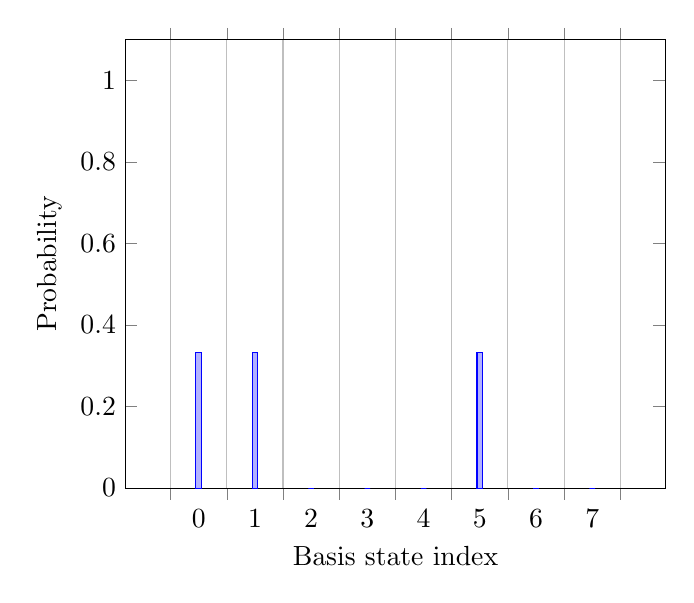
\begin{tikzpicture}
				\begin{axis}[
					ylabel = Probability,
					xlabel = Basis state index,
					ymin = 0,
					ymax = 1.1,
					ybar,
					ybar interval=0.1
				]
				\addplot 
					coordinates {(0,0.333333333333) (1,0.333333333333) (2,0) (3,0) (4,0) (5,0.333333333333) (6,0 ) (7,0) (8,1)};
				\end{axis}
			\end{tikzpicture}
			\caption{Probability distribution for convolution of $\text{T}_a = 11000100$ and $\overline{\text{P}}_a = 10000000$.}
			\label{fig:convolution-a-appendix}
		\end{figure}
	
Again, note that $0.333333333333 = \frac{1}{3}$ and $3.85185988877e^{-34} \approx 0$. Then, the only possible resulting values of a measurement operation on the current state of register $\alpha$ will be the indices 0, 1 and 5. These values correspond to the substrings $\text{T}_a[0, 0] = 1$, $\text{T}_a[0,1] = 11$ and $\text{T}_a[3,5] = 001$.
\end{example}

\begin{example}
\label{exa:aqc-b}
We compute for the convolution of the binary indicator sequences $\text{T}_b$ and $\overline{\text{P}}_b$ given the superposition states $\vert \alpha_b \rangle_0$ and $\vert \beta_b \rangle_0$.
\begin{enumerate}
	\item $\vert \alpha_{b} \rangle_1 = QFT\vert \alpha_{b} \rangle_0 $
		\begin{align*}
			&= QFT \left( \sqrt{\frac{1}{3}}\vert 010 \rangle + \sqrt{\frac{1}{3}}\vert 011 \rangle + \sqrt{\frac{1}{3}}\vert 100 \rangle \right) \\
			&= \left(0.612372435696 \right) \vert 000 \rangle + \left( -0.348461712529 - 0.348461712529\ i \right) \vert 001 \rangle\\
			& \quad + \left( 0.204124145232\ i \right) \vert 010 \rangle + \left( -0.0597865779345 + 0.0597865779345\ i \right) \vert 011 \rangle\\
			& \quad + \left( 0.204124145232 \right) \vert 100 \rangle + \left( -0.0597865779345 - 0.0597865779345\ i \right) \vert 101 \rangle\\
			& \quad + \left( -0.204124145232\ i \right) \vert 110 \rangle + \left( -0.348461712529 + 0.348461712529\ i \right) \vert 111 \rangle
		\end{align*}
	\item $\vert \beta_{b} \rangle_1 = QFT\vert \beta_{b} \rangle_0$
		\begin{align*}
			&= QFT \left( \sqrt{\frac{1}{2}}\vert 001 \rangle + \sqrt{\frac{1}{2}}\vert 010 \rangle \right)\\
			&= \left( 0.5 \right) \vert 000 \rangle + \left( 0.176776695297 - 0.426776695297\ i \right) \vert 001 \rangle\\
			& \quad + \left( -0.25 - 0.25\ i \right) \vert 010 \rangle + \left( -0.176776695297 + 0.0732233047034\ i \right) \vert 011 \rangle\\
			& \quad + \left( 0 \right) \vert 100 \rangle + \left( -0.176776695297 - 0.0732233047034\ i \right) \vert 101 \rangle\\
			& \quad + \left( -0.25 + 0.25\ i \right) \vert 110 \rangle + \left( 0.176776695297 + 0.426776695297\ i \right) \vert 111 \rangle
		\end{align*}
	\item $\vert \alpha_{b} \rangle_2 = V_\beta \vert \alpha_{b} \rangle_1$
		\begin{align*}
			&= V_\beta \Big( \left( 0.5 \right) \vert 000 \rangle + \left( 0.176776695297 - 0.426776695297\ i \right) \vert 001 \rangle\\
			& \quad + \left( -0.25 - 0.25\ i \right) \vert 010 \rangle + \left( -0.176776695297 + 0.0732233047034\ i \right) \vert 011 \rangle\\
			& \quad + \left( 0 \right) \vert 100 \rangle + \left( -0.176776695297 - 0.0732233047034\ i \right) \vert 101 \rangle\\
			& \quad + \left( -0.25 + 0.25\ i \right) \vert 110 \rangle + \left( 0.176776695297 + 0.426776695297\ i \right) \vert 111 \rangle \Big)\\
			&= \left( 0.612372435696 \right) \vert 000 \rangle \\
			& \quad + \left( -0.455287168268 + 0.188586119871\ i \right) \vert 001 \rangle \\
			& \quad + \left( 0.144337567297 - 0.144337567297\ i \right) \vert 010 \rangle \\
			& \quad + \left( 0.0323562628193 - 0.0781149285259\ i  \right) \vert 011 \rangle \\
			& \quad + \left( 0.204124145232\ i \right) \vert 100 \rangle \\
			& \quad + \left( 0.0323562628193 + 0.0781149285259\ i  \right) \vert 101 \rangle\\
			& \quad + \left( 0.144337567297 + 0.144337567297\ i \right) \vert 110 \rangle \\
			& \quad + \left( -0.455287168268 - 0.188586119871\ i \right) \vert 111 \rangle 
		\end{align*}
	\item $\vert \alpha_{b} \rangle_3 = QFT^{-1}\vert \alpha_{b} \rangle_2$
		\begin{align*}
			&= QFT^{-1}\Big( \left( 0.612372435696 \right) \vert 000 \rangle + \left( -0.455287168268 + 0.188586119871\ i \right) \vert 001 \rangle \\
			& \quad + \left( 0.144337567297 - 0.144337567297\ i \right) \vert 010 \rangle \\
			& \quad + \left( 0.0323562628193 - 0.0781149285259\ i  \right) \vert 011 \rangle + \left( 0.204124145232\ i \right) \vert 100 \rangle \\
			& \quad + \left( 0.0323562628193 + 0.0781149285259\ i  \right) \vert 101 \rangle\\
			& \quad + \left( 0.144337567297 + 0.144337567297\ i \right) \vert 110 \rangle \\
			& \quad + \left( -0.455287168268 - 0.188586119871\ i \right) \vert 111 \rangle \Big)\\
			&= (0.0195111123457 + 0.0721687836487\ i ) \vert 000 \rangle \\
			& \quad + (0.0195111123457 - 0.0721687836487\ i) \vert 001 \rangle \\
			& \quad + (-0.074141841541 + 0.0721687836487\ i) \vert 010 \rangle \\
			& \quad + (0.303030398201 - 0.0721687836487\ i) \vert 011 \rangle \\
			& \quad + (0.617625734778 + 0.0721687836487\ i) \vert 100 \rangle \\
			& \quad + (0.617625734778 - 0.0721687836487\ i) \vert 101 \rangle \\
			& \quad + (0.303030398201 + 0.0721687836487\ i) \vert 110 \rangle \\
			& \quad + (-0.074141841541 - 0.0721687836487\ i) \vert 111 \rangle
		\end{align*}
\end{enumerate}
The final state of register $\alpha$ which represents the convolution of the binary indicator sequences $\text{T}_b$ and $\overline{\text{P}}_b$ will be the quantum superposition state $\vert \alpha_{b} \rangle_3$. Each substring $\text{T}_b [j-M-1,j]$ compared to $P_b = 110$ such that $\text{T}_b [j]$ is aligned with $\text{P}_b[M-1]$, and their corresponding basis state's amplitude and probability are shown in Table~\ref{tab:convolution-b-appendix}. A probability distribution corresponding to the convolution of $\text{T}_b$ and $\overline{\text{P}}_b$ is shown in Figure~\ref{fig:convolution-b-appendix}.

	\begin{table}[h!]
	\begin{center}
	\begin{tabular}{|| c | c | c | c ||}
		\hline 
		\textit{j} & $\text{T}_b [j-M-1,j]$ & $\langle i \vert \alpha_{b_3} \rangle$ &  $\vert \langle i \vert \alpha_{b_3} \rangle \vert^2$\\
		\hline\hline
			0 & 0	  & 0.0195111123457 + 0.0721687836487\ i & 0.0055890168383\\
		\hline
			1 & 00   & 0.0195111123457 - 0.0721687836487\ i & 0.0055890168383\\
		\hline
			2 & 001 & -0.074141841541 + 0.0721687836487\ i & 0.0107053460004\\
		\hline
			3 & 011 & 0.303030398201 - 0.0721687836487\ i   & 0.0970357555674\\
		\hline
			4 & 111 & 0.617625734778 + 0.0721687836487\ i  & 0.386669881594\\
		\hline
			5 & 110 & 0.617625734778 - 0.0721687836487\ i   & 0.386669881594\\
		\hline
			6 & 00   & 0.303030398201 + 0.0721687836487\ i  & 0.0970357555674\\
		\hline
			7 & 0    & -0.074141841541 - 0.0721687836487\ i  & 0.0107053460004\\
		\hline
	\end{tabular}
	\end{center}
	\caption{Comparison result between $\text{T}_b = 001110$ and $P_b = 110$.}
	\label{tab:convolution-b-appendix}
	\end{table}

		\begin{figure}
			\centering
			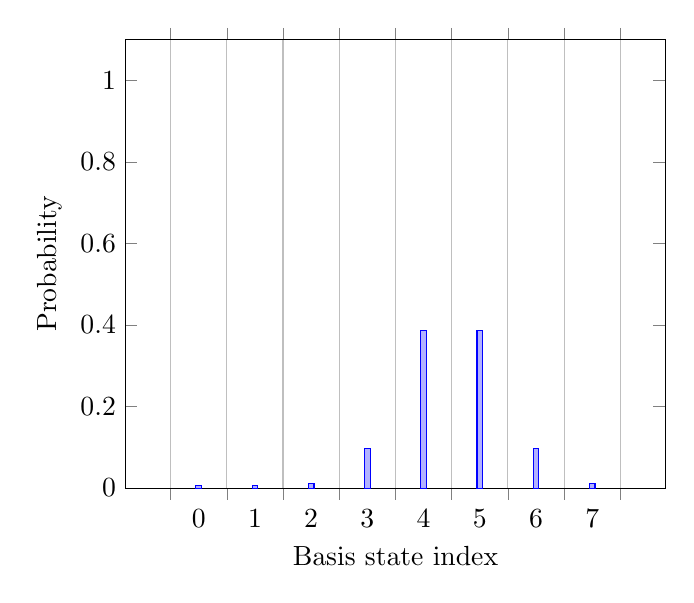
\begin{tikzpicture}
				\begin{axis}[
					ylabel = Probability,
					xlabel = Basis state index,
					ymin = 0,
					ymax = 1.1,
					ybar,
					ybar interval=0.1
				]
				\addplot 
					coordinates {(0,0.0055890168383) (1,0.0055890168383) (2,0.0107053460004) (3,0.0970357555674) (4,0.386669881594) (5,0.386669881594) (6,0.0970357555674 ) (7,0.0107053460004) (8,0)};
				\end{axis}
			\end{tikzpicture}
			\caption{Probability distribution for convolution of $\text{T}_b = 00111000$ and $\overline{\text{P}}_b = 01100000$.}
			\label{fig:convolution-b-appendix}
		\end{figure}

As shown in Table~\ref{tab:convolution-b-appendix} the substrings $\text{T}_b [j-M-1, j]$ with highest probability of occurring from a measurement operation of state of register $\alpha$ are first those for which $j=4$ and $j=5$, followed by those for which $j=3$ and $j=6$, then that for which $j=7$ and $j=2$ and lastly, that for which $j=1$ and $j=0$.
\end{example}

                \chapter{Filtering-based algorithm for approximate string matching}\label{chap:filtering}
                    % In the previous two chapters we presented quantum algorithms which tried to find exact or approximate copies of P in T in the whole search space $\{0,\ldots,N-1\}$. In this chapter we present a quantum algorithm for minimizing the search space by removing elements of the space which do not satisfy a specific criteria. We present a quantum algorithm for the approximate string matching problem which outputs an index \textit{i} in T satisfying the distance threshold requirement with probability directly proportional to the number of matching distinct symbols in P and the substring of T. We use the alphabet $\Sigma=\{a,b,c,d\}$, text $\text{T}= abccabcd$, pattern $\text{P}= abcd$, and distance threshold $d=1$ all throughout this chapter for illustration purposes.

\todo{list explicit contributions}

%The quantum algorithm presented in Chapter \ref{chapter:quantum-convolution} is better suited for instances of the approximate string matching problem in which the size of $\Sigma$ is small since the initial quantum superposition states need to be initialized for T and P for each symbol $\sigma \in \Sigma$. In this chapter we present a quantum algorithm which assumes a an alphabet of large size and a pattern P reach in symbols from $\Sigma$. We use the alphabet $\Sigma=\{a,b,c,d\}$, text $\text{T}= dcbcbaa$, pattern $\text{P}= cbad$ and distance threshold $d=1$ all through out this chapter for illustration purposes.

%%%%%%%%%%%%%%%%%%%%%%%%%%%%%%%%%% Filtering phase %%%%%%%%%%%%%%%%%%%%%%%%%%%%%%%%%%
%\section{Filtering phase}\label{sec:filtering-phase}
\section{Preliminary: A classical filtering algorithm}\label{subsec:filtering-phase-preliminaries}
A. Amir, M. Lewenstein and E. Porat in \cite{Amir2004} proposed a classical algorithm which minimizes the solution space of a string matching problem with specified number of mismatches. We use the following notation in order to explain the filtering concept in the classical algorithm of Amir et al. Let 
\begin{itemize}
	\item $\text{P}_{\Sigma} = \{\alpha_1,\alpha_2, \ldots, \alpha_{q}\}$, $\vert \mathrm{P}_{\Sigma} \vert = q$, set containing all distinct symbols in P
	\item $\text{P}_{\Sigma}^{2d} = $ set containing arbitrary 2\textit{d} elements of the set $\text{P}_{\Sigma}$
	\item $\gamma: \text{P}_{\Sigma} \rightarrow \{0,\ldots,M-1\}; \gamma(\alpha_{j}) = i$ such that $\alpha_{j} \neq \text{P}[k]$ for $0 \leq k < i < M$
\end{itemize}
$\gamma(\cdot)$ is a mapping between elements of $\text{P}_{\Sigma}$ and their index of first occurrence in P.
%We define two sets $P_{\mathrm{Sym}}$ and $P_{\mathrm{Loc}}$. Let $P_{\mathrm{Sym}}$ be the set of all distinct symbols in P. Let $P_{\mathrm{Loc}}$ be the set of indices of first occurrence in P of each symbol in $P_{\mathrm{Sym}}$.  Let both sets be totally ordered such that for any two symbols $x$ and $y$ in $P_{\mathrm{Sym}}$ and two indices $k$ and $l$ in $P_{\mathrm{Loc}}$, $x$ precedes $y$ in $P_{\mathrm{Sym}}$ and $k$ precedes $l$ in $P_{\mathrm{Loc}}$ only if $T[k]=x$, $T[l]=y$ and $k < l$. Let $\vert P_{\mathrm{Sym}} \vert = \vert P_{\mathrm{Loc}} \vert = q$. We denote the $i$-th symbol element of $P_{\mathrm{Sym}}$ to be $P_{\mathrm{Sym}_i}$ and the $i$-th element of $P_{\mathrm{Loc}}$ to be $P_{\mathrm{Loc}_i}$ for $1 \leq i \leq q$.
%substring
%Let $P_{\mathrm{Sym}}$ be the set of distinct symbols in P. Let $P_{\mathrm{Sym}}$ be a totally ordered set such that for any two symbols $P_{\mathrm{Sym}}(i)$, and $P_{\mathrm{Sym}}(j)$, symbol $P_{\mathrm{Sym}}(i)$ precedes symbol $P_{\mathrm{Sym}}(j)$ in set $P_{\mathrm{Sym}}$ only if $P[k]=P_{\mathrm{Sym}}(i), P[l]=P_{\mathrm{Sym}}(j)$ and $k < l$. Let $\vert P_{\mathrm{Sym}} \vert = q$. Let $P_{\mathrm{Loc}}$ be the set of location of first occurrence in P of each symbol in $P_{\mathrm{Sym}}$. Let $P_{\mathrm{Loc}}$ also be a totally ordered set. Given $P_{\mathrm{Sym}}$ and $P_{\mathrm{Loc}}$ we define a mapping $\phi: P_{\mathrm{Sym}} \rightarrow P_{\mathrm{Loc}}$ such that $\phi(P_{\mathrm{Sym}}(i)) = P_{\mathrm{Loc}}(i) \  \forall i, 1 \leq i \leq q$. We assume that $q \geq 2d$. In our example instance, $P_{\mathrm{Sym}}=\{a,b,c,d\}$ and $P_{\mathrm{Loc}}=\{0,1,2,3\}$, $q=4$. Mapping $\phi$ is defined such that $\phi(a)=0, \phi(a)=1, \phi(a)=2, \phi(a)=3$. 

%Let $A=\{\sigma_1, \sigma_2, \ldots, \sigma_q\}$ be a set of all distinct symbols in $\Sigma$ found in P. Let $\vert A \vert = q \geq 2d$. Also, let $A_{loc}=\{j_{\sigma_1}, j_{\sigma_2}, \ldots, j_{\sigma_q} \}$ be the set of locations in P corresponding to the distinct symbols in $A$ such that $P[i_{\sigma_k}] = \sigma_k$ and there exists no other location $0 \leq i < i_{\sigma_k}$ where $P[i] = \sigma_k$. In the quantum algorithm we assume that we can look into sets $A$ and $A_{loc}$ any time as databases in unit time step. Given P, set $A$ is defined to be the set $A=\{a,b,c,d\}$ and the set of locations of symbols in $A$ is defined to be the set $A_{loc}=\{2,1,0,3\}$. We see that $\vert A \vert = 4 $ and $\vert A \vert > 2d$.
In \cite{Amir2004} the elements of $\text{P}_{\Sigma}^{2d}$ is limited only to $2d$ distinct symbols in P. Given a symbol $\mathrm{T}[i]$ and index $\gamma(\mathrm{T}[i])$, index $(i - \gamma(\mathrm{T}[i]))$ in T indicates a possible starting location of P in T. We can slide through T starting at index 0 up to index \textit{N}-1 and evaluate and record the value $(i - \gamma(\mathrm{T}[i]))$ at each index \textit{i}. After the evaluation of each index \textit{i} in T, starting locations of occurrences of P in T will correspond to the most frequently occurring indices $(i - \gamma(\mathrm{T}[i]))$ in our record. We can imagine this process as having \textit{N} buckets labelled from $j=0,\ldots,N-1$ in which we drop a ball in bucket \textit{j} whenever $j=i-\gamma(\mathrm{T}[i])$. The label of the buckets with most number of balls will correspond to a probable starting location of an exact or approximate copy of P in T. Figure~\ref{fig:Amir-filtering-algorithm} illustrates how the classical algorithm of Amir et al. works. We denote the count of points for each index $(i - \gamma(\mathrm{T}[i]))$ in T as $count(i - \gamma(\mathrm{T}[i]))$. Only indices $(i - \gamma(\mathrm{T}[i]))$ in T which satisfies the condition
\begin{equation}\label{eqn:count}
	count(i - \gamma(\mathrm{T}[i])) \geq d
\end{equation}
will be subjected to classical verification in a succeeding phase. The number of remaining indices after the verification phase is bounded above as given in Lemma~\ref{lem:Amir-filtering-algorithm-remaining-locations}.

\begin{figure}[h!]
	\centering
	\includegraphics[scale=0.4]{Amir-filtering-algorithm.png}
	\caption{The classical filtering algorithm in \cite{Amir2004} can be thought of dropping a ball to bucket \textit{j} whenever $j=i - \gamma(\mathrm{T}[i])$. In the example instance where T=\textit{abccabcd}, P=\textit{abcd} and $d=1$, $\mathrm{P}_{\Sigma}^{2d} = \{a,b\}, \vert \mathrm{P}_{\Sigma}^{2d} \vert = 2d = 2$. Also, $\gamma(a)=0,\gamma(b)=1$. Sliding from index 0 to index 7 of T will result to bucket 0 and bucket 4 having 2 points each. Only bucket 0 and bucket 4 satisfies Equation~\ref{eqn:count} and will continue on to the verification phase.}
	\label{fig:Amir-filtering-algorithm}
\end{figure}

%By subtracting the index of first occurrence of symbol $\text{T}[i]$, $\gamma(\text{T}[i])$, from its index \textit{i} in T, i.e. $i - \gamma(\text{T}[i])$, the algorithm is able to identify a possible starting index of P in T. For each computed index $i - \gamma(\text{T}[i])$ in T a \textit{mark} is accounted to. Let $count\left(i - \gamma(\text{T}[i])\right)$ be the count of marks accounted to an index $i - \gamma(\text{T}[i])$. $count\left(i - \text{T}[i]\right) < d$ implies $H\left(\text{T}[i-\gamma(\text{T}[i]),\ldots,i - \gamma(\text{T}[i]) + M -1],\text{P}\right) > d$. Only indices \textit{i} in T where $count\left(i - \gamma(\text{T}[i])\right) \geq d$ will be passed into the verification phase. This minimizes the size of the search space for verification up to an upper bound as stated in Lemma~\ref{lem:remaining-locations-classical}.

%In the classical algorithm in \cite{Amir2004} the elements of $P_{\mathrm{Sym}}$ is limited only to $2d$ number of distinct symbols in P and so $q=2d$. To filter the search space for the problem each symbol $\text{T}[i]$ in T is checked for its index of first occurrence in P using $P_{\mathrm{Sym}}$ and $P_{\mathrm{Loc}}$. If a symbol $\text{T}[i]$ is in $P_{\mathrm{Sym}}$ then its index of first occurrence in P is given by $\phi(\text{T}[i])$. By subtracting the identified index of first occurrence $\phi(\text{T}[i])$ of a symbol $\text{T}[i]$ from its index \textit{i} in T, i.e. $i - \phi(\text{T}[i])$, the algorithm is able to identify a possible starting index of P in T. For each computed index $i - \phi(\text{T}[i])$ in T a mark is accounted to. An index $i - \phi(\text{T}[i]$ with count of marks less than $2d$ implies a starting index for an M-length substring in T with number of mismatches when compared to P to be greater than \textit{d}. In the filtering phase of the classical algorithm in \cite{Amir2004} only indices $i - \phi(\text{T}[i])$ in T with count of marks greater than or equal to $d$ are qualified to be passed into the verification phase. This minimizes the size of the search space for the verification phase up to an upper bound as stated in Lemma~\ref{lem:remaining-locations-classical}.

%In \cite{Amir2004} the set $A$ is limited to a chosen $2d$ distinct symbols in P and thus $\vert A \vert = \vert A_{loc} \vert = 2d$. Given $A$ and $A_{loc}$, each location $i$ in T is queried for its symbol $\text{T}[i]$ from $A$ and then $A_{loc}$ is queried for the location $j_{T[i]}$ of the symbol $\text{T}[i]$'s first occurrence in P. A mark is then accounted to location $i - j_{T[i]}$. After all the locations in T has been evaluated, locations with fewer than $d$ marks are discarded since it implies that substrings of T which start at these locations have $d$ or more mismatches. An upper bound on the number of remaining locations in T after the filtering phase is stated in \ref{lem:remaining-locations-classical}.

\begin{lemma}[\cite{Amir2004}]
\label{lem:Amir-filtering-algorithm-remaining-locations}
	At the conclusion of the filtering phase there are at most $\frac{N}{d}$ remaining indices of text T for verification.
\end{lemma}
\begin{proof}
	Since the filtering algorithm makes a total of \textit{N} points and the \textit{M}-length substrings of T starting at every remaining index has at least \textit{d} marks, it implies that at most $\frac{N}{d}$ indices in T will remain.
\end{proof}

\subsection{Quantum filtering}
We look into the operation of the filtering step of the algorithm of Amir et al. in the quantum circuit model. Instead of restricting the operation of the step into the set $\text{P}_{\Sigma}^{2d}$ we consider the set $\text{P}_{\Sigma}$, i.e. $q \geq 2d$. All candidate solutions in quantum computing cannot be produced simultaneously as output of a quantum algorithm. We can only mark each candidate solution and produce one of these classical solutions using a measurement operation. We thus need to reformulate the statement pertaining to the upper bound on the number of remaining locations in T after an execution of the filtering step in the quantum setting with consideration to this output restriction.

\begin{lemma}
The execution of the quantum filtering step will mark at most $\frac{N}{q-d}$ indices in T.
\end{lemma}
\begin{proof}
Proof here.
\end{proof}
\begin{proof}
	Since the filtering operation in the quantum circuit model makes a total of \textit{N} points and since every remaining index in T has at least $q-d$ marks it implies that at most $\frac{N}{q-d}$ indices remain.
\end{proof}

The application of Lemma~\ref{lem:quantum-filtering-algorithm-remaining-locations} to our sample instance is shown in Figure~\ref{fig:quantum-filtering-algorithm}.
\begin{figure}[h!]
	\centering
	\includegraphics[scale=0.4]{quantum-filtering-algorithm.png}
	\caption{The quantum filtering algorithm includes all distinct symbols in P. In the example instance where T=\textit{abccabcd}, P=\textit{abcd} and $d=1$, $\mathrm{P}_{\mathrm{Sym}} = \{a,b\}, \vert \mathrm{P}_{\mathrm{Sym}} \vert = 4$. Also, $\gamma(a)=0,\gamma(b)=1,\gamma(c)=2, \gamma(d)=3$. Sliding from index 0 to index 7 of T will result to bucket 0 having 3 points and bucket 4 with 4 points. Only bucket 0 and bucket 4 satisfies Equation~\ref{eqn:count} and will continue on to the verification phase.}
	\label{fig:quantum-filtering-algorithm}
\end{figure}

%In application to our example instance we compute for the locations $i - i_j$ as shown in Table~\ref{tab:start-locations}.
%\begin{table}[h!]
%	\begin{center}
%		\begin{tabular}{|| c | c | c | c ||}
%					\hline
%					$i$ & $\text{T}[i]$ & $\gamma(\text{T}[i])$ & $i-\gamma(\text{T}[i])$ \\
%					\hline
%					\hline			
%					 0	  &	a					&		0						&	0							\\
%					 \hline
%					 1	  &	b					&		1						&	0							\\
%					\hline 
%					 2	  &	c					&		2						&	0							\\
%					\hline 
%					 3	  &	c					&		2						&	1							\\
%					\hline 
%					 4	  &	a					&		0						&	4							\\
%					\hline 
%					 5	  &	b					&		1						&	4							\\
%					\hline 
%					 6	  & 	c					&		2						&	4							\\	
%					\hline
%					 7	  & 	d					&		3						&	4							\\	
%					\hline
%		\end{tabular}
%	\end{center}
%	\caption{Computation of values $i-\gamma(\text{T}[i])$ for sample input instance. Index $i-\gamma(\text{T}[i])=0$ has three marks accounted to it, index $i-\gamma(\text{T}[i])=1$ has one and index $i-\gamma(\text{T}[i])=4$ has four marks. The input threshold distance is $d=2$. The classical filtering algorithm will output $\frac{N}{d}=\frac{8}{2}=2$ indices $i-\gamma(\text{T}[i])$. Same will be the output for the quantum algorithm, $\frac{N}{q-d}=\frac{8}{4-2}=2$.}
%	\label{tab:start-locations}
%\end{table}

\section{Outline}
We discuss the outline of the quantum filtering step in this section and the details of each unitary operator used in the algorithm in the succeeding sections. We start off by initializing two quantum registers which we name as follows
\begin{itemize}
	\item \textit{index register}
		\begin{itemize}
			\item the state of which will represent all indices \textit{i} in T
			\item composed of $n=\log_{2}(N)$ qubits for representing values $0,\ldots,N-1$
			\item initialized into state $\vert \mathbf{0} \rangle = \vert 0 \rangle^{\otimes n}$, decimal representation of the 0 state
		\end{itemize}
	\item \textit{start register}
		\begin{itemize}
			\item the state of which will represent indices $\gamma(\text{T}[i])$ in P and eventually the indices $i - \gamma(\text{T}[i])$ in T
			\item composed of $n+1$ qubits for representing values $-N,\ldots,0,\ldots,N-1$
			\item initialized into state $\vert \mathbf{0} \rangle=\vert 0 \rangle^{\otimes n+1}$
		\end{itemize}
\end{itemize}
The initial state of the two registers will be 
\begin{align}
	\label{eqn:zero-state}
	\vert \psi \rangle = \vert \mathbf{0} \rangle\vert \mathbf{0} \rangle
\end{align}

We encode the result of the computation of the value $(i-\gamma(\mathrm{T}[i]))$ for all $i=0,\ldots,N-1$ in T using the state of the two registers. We first put the registers into the uniform superposition state
\begin{align}
	\label{eqn:superposition-state}
	\vert \psi_{\mathrm{init}} \rangle = \frac{1}{\sqrt{N}} \sum_{i=0}^{N-1} \vert i \rangle \vert \mathbf{0} \rangle
\end{align}
Assuming that $\text{P}_{\Sigma}$ has already been prepared prior to the quantum computation we perform the evaluation of each substring $\mathrm{T}[i],\ldots,\mathrm{T}[i+M-1]$ using a unitary operator applied to state $\vert \psi_{\mathrm{init}} \rangle$. The identification of the index $\gamma(\text{T}[i])$ in P for each index \textit{i} in T can be viewed as a query task. We use a unitary operator $U_{\sigma}$ to facilitate this effect into the quantum registers in state $\vert \psi_{\mathrm{init}} \rangle$. Each identified index $\gamma(\text{T}[i])$ is represented with the state of the start register, $\vert \gamma(\text{T}[i]) \rangle$. The resulting superposition state from application of operator $U_{\sigma}$ into the two registers will be
\begin{align}\label{eqn:psi-loc}
	\vert \psi_{\mathrm{loc}} \rangle = \frac{1}{\sqrt{N}} \sum_{i=0}^{N-1} \vert i \rangle \vert \gamma(\text{T}[i]) \rangle
\end{align}

%The identification of the location $\phi(\text{T}[i])$ for each location $i$ in T represented by each state $\vert i \rangle$ can be interpreted as a querying task since we assume that sets $P_{\mathrm{Sym}}$ and $P_{\mathrm{Loc}}$ were prepared prior to computation. We use a unitary operator $U_{\mathrm{Loc}}$ to facilitate this effect on the quantum registers in state $\vert \psi_{\mathrm{init}} \rangle$. Given location $i$ in T this operator facilitates the querying of each location $\phi(\text{T}[i])$ from set $P_{\mathrm{Loc}}$. Each identified first occurrence location $\phi(\text{T}[i])$ is loaded into the second register, initially in state $\vert \mathbf{0} \rangle$. Since the utility of this operator is for querying the readily accessible sets $P_{\mathrm{Sym}}$ and $P_{\mathrm{Loc}}$ we assume a unit time step operation for this operator. The resulting state from application of operator $U_{\mathrm{Loc}}$ into state $\vert \psi_{\mathrm{init}} \rangle$ is the state
%\begin{align}
%	\label{eqn:location-state-1}
%	\vert \psi_{\mathrm{loc}} \rangle = \sqrt{\frac{1}{N}} \sum_{i=0}^{N-1} \vert i \rangle \vert \phi(\text{T}[i]) \rangle
%\end{align}

We compute each index $(i - \gamma(\text{T}[i]))$ in T using another operator, $U_{\mathrm{Sub}}$. Given the quantum state $\vert \psi_{\mathrm{loc}} \rangle$, $U_{\mathrm{Sub}}$ facilitates the computation of each value $(i - \gamma(\text{T}[i]))$ and encodes it into the state of the start register. The superposition state resulting from application of $U_{\mathrm{Sub}}$ into state $\vert \psi_{\mathrm{loc}} \rangle$ is the state
\begin{align}\label{eqn:psi-sub}
	\vert \psi_{\mathrm{sub}} \rangle = \frac{1}{\sqrt{N}} \sum_{i=0}^{N-1} \vert i \rangle \vert i - \gamma(\text{T}[i]) \rangle
\end{align}
We may in concept implement operator $U_{\mathrm{Sub}}$ using the design of a quantum adder in \cite{Barenco1996}. We discuss the details of implementation of operator $U_{\mathrm{Sub}}$ using the design in \cite{Barenco1996} in Section~\ref{sec:u_sub}.

In the classical filtering step of Amir et al. we count the resulting number of points for each index $(i - \gamma(\text{T}[i]))$ in T. In our quantum filtering step we can rewrite the summation in state $\vert \psi_{\mathrm{sub}} \rangle$  as a summation of summations such that states $\vert i \rangle$ of index register with same associated state $\vert i - \gamma(\text{T}[i]) \rangle$ for start register are grouped together in form of summations,
\begin{align}\label{eqn:psi-sub-sum}
	\vert \psi_{\mathrm{sub}} \rangle = \sqrt{\frac{c_{i_1}}{N}} \sum_{i, (i- \gamma(\text{T}[i]))=i_1} \vert i \rangle \vert i_1 \rangle + \sqrt{\frac{c_{i_2}}{N}} \sum_{i, (i- \gamma(\text{T}[i]))=i_2} \vert i \rangle \vert i_2 \rangle + \ldots + \sqrt{\frac{c_{i_m}}{N}} \sum_{i, (i-\gamma(\text{T}[i]))=i_m} \vert i \rangle \vert i_m \rangle
\end{align}
where $c_{i_k} = count\left( i_k \right)$, $1 \leq k \leq m$, is the count of points of index $i_k$ in T. Indices $i_k$ which have higher count of points will have greater amplitude as compared to those states which have lower count of points in the superposition state $\vert \psi_{\mathrm{sub}} \rangle$. In the classical filtering step of Amir et al. we discard indices $i_k$ where $count(i_k) < d$ and we retain at most $\frac{N}{d}$ indices. In the quantum filtering step we cannot deterministically select and retain the indices $i_k$ which have $count(i_k) \geq q-d$ since we are working with a superposition of states. Instead, we iterate the quantum filtering step until we get $\frac{N}{q-d}$ distinct indices. With high probability we get the indices $i_k$ in T which satisfy the condition $count(i_k) \geq q-d$.

In the succeeding sections we discuss the details of the unitary operators used in each step in the quantum filtering phase.

%%%%%%%%%%%%%%%%%%%%%%%%%%%%%%%%%% Unitary operator U_Loc %%%%%%%%%%%%%%%%%%%%%%%%%%%%%%%%%%
\section{Quantum filtering phase sub-routines}
\subsection{Identification of each symbol $\mathrm{T}[i]$}
We assume that text T is accessible through a memory device abstracted using the QRAM model implemented using the bucket brigade architecture \cite{Giovannetti2008b}. We provide the quantum superposition state $\vert \psi_{\mathrm{init}} \rangle = \frac{1}{\sqrt{N}} \sum_{i=0}^{N-1} \vert i \rangle$ as input to the address register of QRAM. We get as output of QRAM a superposition state
\[
	\vert \psi_{\mathrm{ram}} \rangle = \frac{1}{\sqrt{N}} \sum_{i=0}^{N-1} \vert i \rangle\vert 0 \rangle\vert \mathrm{T}[i] \rangle
\]
where each symbol $\mathrm{T}[i]$ is encoded as the state of QRAM's output register. 
\todo{Move this content to the dedicated section for QRAM in the preliminaries for quantum computing}
QRAM implemented using the bucket brigade architecture has a circuit complexity in $\Om(N)$ but has circuit depth of only $\Om(\log N)$. Its time complexity for each query will then also be in $\Om(\log N)$. It has a space complexity of $\Om(N)$. 

\subsection{Identification of each location of first occurrence $\gamma(\sigma_i)$}
To identify the location of first occurrence of each symbol $\mathrm{T}[i]$ in $\vert \psi_{\mathrm{ram}} \rangle$, $\lambda(\mathrm{T}[i])$,we construct controlled \textit{location operators} $U_{\sigma_k}$ for $k=1,\ldots,\vert \Sigma \vert$. The qubits of the output register of QRAM will serve as control qubits of each of the controlled location operators $U_{\sigma_k}$. Given a symbol $\sigma_k$ as input state only operator $U_{\sigma_k}$ will be activated and will transform the state of the start register from its initial state $\vert \mathbf{0} \rangle$ into the state $\vert \gamma(\sigma_k) \rangle$. Since the state $\vert \psi_{\mathrm{ram}} \rangle$ is a superposition of states the location operators will be applied linearly to each state $\vert i \rangle\vert 0 \rangle\vert \mathrm{T}[i] \rangle$ in $\vert \psi_{\mathrm{ram}} \rangle$. The resulting state from the operation of the location operators $U_{\sigma_k}$ on state $\vert \psi_{\mathrm{ram}} \rangle$ will be the superposition state
\[
	\vert \psi_{\mathrm{loc}} \rangle = \frac{1}{\sqrt{N}} \sum_{i=0}^{N-1} \vert i \rangle\vert \gamma(\mathrm{T}[i]) \rangle \vert \mathrm{T}[i] \rangle
\]
for all $i=0,\ldots,N-1$. A quantum circuit for a controlled location operator $U_{\sigma_k}$ is illustrated in Figure~\ref{fig:location-operator}.
\begin{figure}[ht]
	\centering
	\footnotesize
	\begin{minipage}[b]{0.8\linewidth}
		\[
			\Qcircuit @C=1em @R=1em {
				& \quad                                     & \quad & \qw & \ctrl{1}                                 & \qw  & \quad & \quad \\
				& \lstick{\vert \sigma_k \rangle} & \quad & \qw & \ctrl{1}                                 & \qw & \quad & \quad \vert \sigma_k \rangle \\
				& \quad                                      & \quad & \qw & \ctrl{1}                                 & \qw & \quad & \quad \\
				& \lstick{\vert 0 \rangle}             & \quad & \qw & \multigate{2}{U_{\sigma_k}} & \qw & \quad & \quad \\
				& \lstick{\vert 0 \rangle}             & \quad & \qw & \ghost{U_{\sigma_k}}           & \qw & \quad & \quad\quad \vert \gamma(\sigma_k) \rangle \\
				& \lstick{\vert 0 \rangle}             & \quad & \qw & \ghost{U_{\sigma_k}}           & \qw & \quad & \quad\\
				& \lstick{\vert 0 \rangle}             & \quad & \qw & \qw			           & \qw & \quad & \quad\\
				& \lstick{\vert 0 \rangle}             & \quad & \qw & \qw           			& \qw & \quad & \quad
				\gategroup{1}{3}{3}{3}{1em}{\{}\gategroup{4}{6}{8}{6}{1em}{\}} \\
			}		
		\]
	\end{minipage}
	\caption{An example of a quantum circuit for a location operator $U_{\sigma_k}$ where $\log(\vert \Sigma \vert) = 3$, $\log(M) = 3$ and $\log(N) = 5$. The control qubits in state $\vert \sigma_{k} \rangle$ correspond to the output register of a QRAM which encodes a symbol $\mathrm{T}[i]=\sigma_k$. The state of the control qubits depends on the encoding of the symbol $\sigma_k$. In this figure the encoding of $\sigma_k$ is $\vert 111 \rangle$. The operation of operator $U_{\sigma_k}$ includes only the top $\log(M) = 3$ qubits of the start register where the topmost qubit is the least significant bit.}
	\label{fig:location-operator}
\end{figure}
\begin{claim}\label{cla:U-sigma-multi-cnot}
A $U_{\sigma_k}$ operator can be decomposed into at most $\log(M)$ $C^{\log \vert \Sigma \vert}NOT$ gates.
\end{claim}
\begin{proof}
Each symbol $\sigma_k \in \Sigma$ can be represented using $\log(\vert \Sigma \vert)$ qubits. These qubits make up the output register of the QRAM and will serve as control qubits for our controlled location operators $U_{\sigma_k}$. The range of values of $\gamma(\cdot)$ will be $\{0,\ldots,M-1\}$ and can be represented with $\log(M)$ qubits. Given that the start index is composed of $\log(N) + 1$ qubits and is initiated in state $\vert \mathbf{0} \rangle$, only $\log(M)$ of these qubits at most will be flipped during the operation. We can then decompose our operator $U_{\sigma_k}$ into at most $\log(M)$ $\log(\vert \Sigma \vert)$-qubit controlled \textit{NOT} operators ($C^{\log(\vert \Sigma \vert)}NOT$).
\end{proof}
An illustration of the $C^{\log(\vert \Sigma \vert)}NOT$ decomposition of $U_{\sigma_k}$ is shown in Figure~\ref{fig:location-operator-multi-CNOT}.
\begin{figure}[ht]
	\centering
	\footnotesize
	\begin{minipage}[b]{0.8\linewidth}
		\[
			\Qcircuit @C=1em @R=1em {
				& \quad                                     & \quad & \qw  & \ctrl{1} & \ctrl{1}  & \qw  & \quad \\
				& \lstick{\vert \sigma_k \rangle} & \quad & \qw & \ctrl{1}  & \ctrl{1} & \qw & \quad \vert \sigma_k \rangle \\
				& \quad                                      & \quad & \qw & \ctrl{1}  & \ctrl{2} & \qw & \quad \\
				& \lstick{\vert 0 \rangle}             & \quad & \qw & \targ     & \qw       & \qw & \quad \\
				& \lstick{\vert 0 \rangle}             & \quad & \qw & \qw       & \targ     & \qw & \rstick{\vert \gamma(\sigma_k) \rangle} \\
				& \lstick{\vert 0 \rangle}             & \quad & \qw & \qw       & \qw       & \qw & \quad\\
				& \lstick{\vert 0 \rangle}             & \quad & \qw & \qw       & \qw       & \qw & \quad\\
				& \lstick{\vert 0 \rangle}             & \quad & \qw & \qw       & \qw       & \qw & \quad
				\gategroup{1}{3}{3}{3}{1em}{\{}\gategroup{4}{7}{8}{7}{1em}{\}} \\
			}		
		\]
	\end{minipage}
	\caption{An example of a multi-controlled \textit{NOT} decomposition of the quantum operator $U_{\sigma_k}$ where $\log(\vert \Sigma \vert) = 3$, $\log(M) = 3$ and $\log(N) = 5$. The operation of the $U_{\sigma_k}$ operator on the qubits of the start register flips the state of the top two qubits of the register and keeps the initial state of the third register. This indicates that the location of first occurrence of the symbol $\sigma_{k}$ in P is in index $2^{0} \times 1 + 2^{1} \times 1 = 3$.}
	\label{fig:location-operator-multi-CNOT}
\end{figure}
\begin{lemma}[2-qubit-controlled unitary operator decomposition \cite{Barenco1995b}]\label{lem:2-controlled-not-elementary-decomposition}
For any $2\times 2$ unitary matrix U, $C^{2}U$ gate can be simulated by a network of the form
\begin{figure}[H]
	\centering
	\footnotesize
	\begin{minipage}[b]{0.8\linewidth}
		\begin{align*}
			\Qcircuit @C=1em @R=1em {
				& \ctrl{1} & \qw & \quad  		& \qw		& \ctrl{1}	& \qw			& \ctrl{1}	& \ctrl{2}	& \qw\\
				& \ctrl{1} & \qw & \quad = \quad\quad  & \ctrl{1} 	&  \targ{} 	& \ctrl{1}		& \targ{}	& \qw		& \qw\\
				& \gate{U} & \qw & \quad 		& \gate{V} 	& \qw		& \gate{V^{\dagger}}	& \qw		& \gate{V}	& \qw
			}
		\end{align*}
	\end{minipage}
\end{figure}
where V is unitary.
\end{lemma}
\begin{lemma}[\textit{n}-qubit-controlled unitary operator decomposition \cite{Barenco1995b}]\label{lem:multi-controlled-not-elementary-decomposition}
For any $n \geq 3$ and any unitary $2 \times 2$  matrix \textit{U}, a $C^{n-1}U$ gate can be simulated by an \textit{n}-bit network consisting of $2^{n-1} - 1$ $C^1 V$ and $C^1 V^\dagger$ gates and $2^{n-1} - 2$ \textit{CNOT} gates, where \textit{V} is unitary.
\end{lemma}
Lemma \ref{lem:multi-controlled-not-elementary-decomposition} is a generalization of Lemma~\ref{lem:2-controlled-not-elementary-decomposition} from two qubits to arbitrary \textit{n} control qubits. The decomposition of the controlled $U_{\sigma_{k}}$ gates in Figure~\ref{fig:location-operator-multi-CNOT} requires the use of $C^{\log(\vert\Sigma\vert)}NOT$ gates. A single controlled $U_{\sigma_{k}}$ gate will require $\log(M)$ $C^{\log(\vert\Sigma\vert)}NOT$ gates at most.
\begin{claim}\label{cla:U-sigma-elementary-gates}
A single operator $U_{\sigma_k}$ will require elementary gates in $\Om\left(\vert \Sigma \vert \log(M) \right)$ count.
\end{claim}
\begin{proof}
By Claim~\ref{cla:U-sigma-multi-cnot} each operator $U_{\sigma_k}$ can be decomposed into at most $\log(M)\ C^{\log(\vert \Sigma \vert)}NOT$ gates. Let $n=\log \vert \Sigma \vert$. By Lemma~\ref{lem:multi-controlled-not-elementary-decomposition} we can decompose each $C^{\log(\vert \Sigma \vert)}NOT$ gate into $(\vert \Sigma \vert - 1)$ $C^1 V$ and $C^1 V^\dagger$ gates and $(\vert \Sigma \vert - 2)$ \textit{CNOT} gates where \textit{V} is unitary. Thus, each operator $U_{\sigma_k}$ can be decomposed into $\Om(\vert \Sigma \vert \log(M))$ elementary gates.
\end{proof}
\todo{Determine V when U=X.}

\begin{lemma}\label{lem:U-sigma-circuit-complexity}
The set of operators $U_{\sigma_k}$ for $k=1,\ldots,\vert \Sigma \vert$ can be synthesized into a quantum circuit with elementary gate count in $\Om\left(\vert \Sigma \vert^2\log(M)\right)$.
\end{lemma}
\begin{proof}
By Claim~\ref{cla:U-sigma-elementary-gates} each operator $U_{\sigma_k}$ can be decomposed into $\Om\left(\vert \Sigma \vert \log M \right)$ elementary gates and by our construction we will require $\vert \Sigma \vert$ controlled location operators $U_{\sigma_k}$. We can then synthesize the quantum circuit for all the location operators $U_{\sigma_k}$ with gate count in $\Om\left(\vert \Sigma \vert^2\log(M)\right)$
\end{proof}

\begin{lemma}\label{lem:U-sigma-time-complexity}
The time complexity for the operation of the location operators $U_{\sigma_k}$ will be in $\Om\left(\vert \Sigma \vert \log(M)\right)$.
\end{lemma}
\begin{proof}
During the step for identifying the location of occurrence of symbol $\mathrm{T}[i]$ in P, $\gamma(\mathrm{T}[i])$, only a single operator $U_{\sigma_k}$ will be activated. Thus, only $\Om\left(\vert \Sigma \vert\log(M)\right)$ elementary gates will be activated at a single time.
\end{proof}

%\subsubsection{Unitary operator $U_{\mathrm{Loc}}$}
%We discuss about the details of the design for the unitary operator $U_{\mathrm{Loc}}$. Given state $\vert \psi_{\mathrm{init}} \rangle$ in Equation \ref{eqn:superposition-state}, the application of operator $U_{\mathrm{Loc}}$ will result to state $\vert \psi_{\mathrm{loc}} \rangle$ in Equation \ref{eqn:psi-loc}. Operator $U_{\mathrm{Loc}}$ can be expressed as a matrix representing the mapping of each symbol $\text{T}[i]$ to indices $\gamma(\text{T}[i])$. It will work on the index register and start register states as given by the mapping $\vert i \rangle\vert 0 \rangle \rightarrow \vert i \rangle\vert \gamma(\mathrm{T}[i]) \rangle$ for $i=0,\ldots,N-1$. Since the size of the index register will be $n$ and that of start register will be $n+1$ then the dimension of the unitary matrix for $U_{\mathrm{Loc}}$ will be $\left(2^{n} \times 2^{n+1}\right) \times \left(2^{n} \times 2^{n+1}\right)$. The $2^n$ $2^{n+1} \times 2^{n+1}$ square matrices along the diagonal of this unitary matrix will be sparse permutation matrices with at most one transposition of indices and all 1s along the diagonal. The unitary matrix for $U_{\mathrm{Loc}}$ is then also a sparse permutation matrix with at most \textit{N} transpositions. We denote the $2^{n+1} \times 2^{n+1}$ permutation matrix along the \textit{i}-th block of $2^{n+1}$ rows and \textit{j}-th block of $2^{n+1}$ columns of the unitary matrix for $U_{\mathrm{Loc}}$ as $U_{\mathrm{Loc}}[i,j]$. We label the rows of this permutation matrix as $(i,-N),\ldots,(i,0),\ldots,(i,N-1)$ and its columns as $(j,-N),\ldots,(j,0),\ldots,(j,N-1)$. The sub-matrix of $U_{\mathrm{Loc}}[i,j]$ defined by rows $(i,-N),\ldots,(i,-1)$ and columns $(j,-N),\ldots,(j,-1)$ correspond to negative indices of P and we denote it as $U_{\mathrm{Loc}}^-[i,j]$. Since the range of $\gamma(\cdot)$ is composed only of indices $0,\ldots,M-1$, we let this sub-matrix be an identity matrix. On the other hand, the sub-matrix of $U_{\mathrm{Loc}}[i,j]$ defined by rows $(i,0),\ldots,(i,N-1)$ and columns $(j,0),\ldots,(j,N-1)$ correspond to positive indices in P. We denote this sub-matrix as $U_{\mathrm{Loc}}^+[i,j]$ its elements are given by 
%\begin{align}
%	U_{\mathrm{Loc}}^+[i,j]\left((i,k),(j,l)\right)=
%	\begin{cases}
%		1, & \mathrm{if\ i=j \bigwedge \left(\left(k=0 \wedge \gamma(\mathrm{T[i]})=l\right) \bigvee \left(k \neq 0 \wedge k=l\right)\right) }\\
%		0, & \mathrm{otherwise}
%	\end{cases}
%\end{align}  
%for $k,l=0,\ldots,N-1$.
%%Each contiguous block of $2^{(n+1)}$ rows and columns of the matrix will correspond to a single index $i$ in T. Each row (column) within such block of rows (columns) will correspond to an integer in the range $\{-N,\ldots,0,\ldots,N-1\}$. To facilitate the fetching of indices $\gamma(\text{T}[i])$ given state $\vert i \rangle\vert 0 \rangle$ into state $\vert i \rangle\vert \gamma(\text{T}[i]) \rangle$, a value of 1 will be assigned into each cell $\left([i,0],[i,\gamma(\text{T}[i])]\right)$ and each cell $\left( [i,\gamma(\text{T}[i])],[i,0] \right)$. The other cells in the diagonal be assigned a value of 1 and the rest a value of 0. Based on these rules we define operator $U_{\mathrm{Loc}}$ as the unitary matrix given by
%%\begin{align}
%%	U_{\mathrm{Loc}}(x,y) = 
%%		\begin{cases}
%%			1, & \text{if}\ \left((x,y) = ([i,0],[i,\gamma(\text{T}[i])])\ \mathrm{OR}\ (x,y) = ([i,\gamma(\text{T}[i])],[i,0])\right)\ \mathrm{XOR}\ x=y\\ 
%%			0, & \mathrm{otherwise}
%%		\end{cases}
%%\end{align}
%%for $0 \leq i \leq N-1$. 
%Note that the normalizing factor for the matrix of operator $U_{\mathrm{Loc}}$ is just 1 since it is just a permutation matrix. Thus, application of $U_{\mathrm{Loc}}$ have no effect on the amplitude of the state of the register. 

\begin{example}
Given our example input instance where $\text{P}_{\mathrm{Sym}}=\{a,b,c,d\}$ we define operator $U_{\sigma}$ as the unitary matrix with value 1 in cells [(0,0),(0,0)], [(1,0),(1,1)], [(1,1),(1,0)], [(2,0),(2,2)], [(2,2),(2,0)], [(3,0),(3,2)], [(3,2),(3,0)], [(4,0),(4,0)], [(5,0),(5,1)], [(5,1),(5,0)], [(6,0),(6,2)], [(6,2),(6,0)], [(7,0),(7,3)], [(7,3),(7,0)] and the rest of the diagonal entries not coinciding with the rows of these cells. For brevity we present the matrix of $U_{\sigma}$ for the sample input instance in the Appendix~\ref{app:ULoc}. %Some details on simulation of operator $U_{\mathrm{Loc}}$ will be discussed in Section~\ref{sec:filtering-simulation}. 
The resulting state from application of operator $U_{\sigma}$ will be the state $\vert \psi_{\mathrm{loc}} \rangle$ in Equation~\ref{eqn:psi-loc}. In our input instance the resulting state will be
\begin{align}
	\vert \psi_{\mathrm{loc}} \rangle = \sqrt{\frac{1}{8}}\left( \vert 0 \rangle\vert 0 \rangle + \vert 1 \rangle\vert 1 \rangle + \vert 2 \rangle\vert 2 \rangle + \vert 3 \rangle\vert 2 \rangle + \vert 4 \rangle\vert 0 \rangle + \vert 5 \rangle\vert 1 \rangle + \vert 6 \rangle\vert 2 \rangle + \vert 7 \rangle\vert 3 \rangle\right)
\end{align}
\end{example}
%%%%%%%%%%%%%%%%%%%%%%%%%%%%%%%%%% Unitary operator U_Sub %%%%%%%%%%%%%%%%%%%%%%%%%%%%%%%%%%

\subsection{Identification of each starting location $(i - \gamma(\sigma_i))$}\label{sec:u_sub}
The computation of the state $\vert i-\gamma(\mathrm{T}[i]) \rangle$ in Equation~\ref{eqn:psi-sub} can be implemented using the operator $U_{\mathrm{Sub}}$. Given input state 
\begin{align*}
\vert \psi_{\mathrm{loc}} \rangle &= \frac{1}{\sqrt{N}} \sum_{i=0}^{N-1} \vert i \rangle\vert \gamma(\mathrm{T}[i]) \rangle \vert \mathrm{T}[i] \rangle
\end{align*}
the operator $U_{\mathrm{Sub}}$ transforms the state of the index and start register from $\vert i \rangle\vert \gamma(\mathrm{T}[i]) \rangle$ into a superposition of states $\vert i \rangle\vert i - \gamma(\text{T}[i]) \rangle, 0 \leq i < N$. This operation can be implemented using \textit{component adder} and \textit{complement operators}. A \textit{quantum full-adder} can be implemented using a cascade of \textit{quantum half-adder}. A circuit implementing a quantum half-adder is shown in Figure~\ref{fig:half-adder}.
\begin{figure}[ht]
	\centering
	\begin{minipage}[b]{0.8\linewidth}
		\[
			\Qcircuit @C=1em @R=1em {
				& \lstick{x_i} & \ctrl{2}  & \ctrl{1}   & \qw & \rstick{x_i}         \\
				& \lstick{y_i} & \ctrl{1}  & \gate{X} & \qw & \rstick{x_i + y_i} \\
				& \lstick{0}	  & \gate{X} & \qw        & \qw & \rstick{c_i}        
			}		
		\]
	\end{minipage}
	\caption{A circuit for a quantum half-adder for adding values represented by states of two qubits where addition is done modulo 2. The third qubit is an auxiliary qubit for holding carry value $c_i$.}
	\label{fig:half-adder}
\end{figure}
A circuit for a quantum adder for two qubits with carry value propagation is shown in Figure~\ref{fig:full-adder}.
\begin{figure}[ht]
	\centering
	\begin{minipage}[b]{0.8\linewidth}
		\[
			\Qcircuit @C=1em @R=1em {
				& \lstick{c_{i-1}} & \qw	      & \qw        & \ctrl{4}  & \ctrl{2}  &	\qw         & \qw & \rstick{c_{i-1}}\\
				& \lstick{x_i}       & \ctrl{2}  & \ctrl{1}   & \qw       & \qw        & \qw        & \qw & \rstick{x_i}\\
				& \lstick{y_i}       & \ctrl{1}  & \gate{X} & \ctrl{2}  & \gate{X} & \qw        & \qw & \rstick{z_i}\\
				& \lstick{0}	        & \gate{X} & \qw        & \qw       & \qw        & \ctrl{1}   & \qw & \rstick{x_i \wedge y_i} \\
				& \lstick{0}         & \qw        & \qw        & \gate{X} & \qw       &	\gate{X} & \qw & \rstick{c_i}
			}		
		\]
	\end{minipage}
	\caption{A quantum circuit for adding two binary values represented by states of two qubits where addition is performed modulo 2. The carry values are propagated through scratch qubits initially set to state 0. $z_i = x_i + y_i + c_{i-1}$ and $c_i$ is the total carry resulting from the addition.}
	\label{fig:full-adder}
\end{figure}
The circuit for adding two qubits of information makes use of one auxiliary qubit for scratch and one carry qubit. We allot an auxiliary register composed of a multiple of two qubits with exact count depending on the pre-fixed size of the index and start registers. The circuit for this adder is based on what was proposed in \cite{Barenco1996} for a  \textit{full quantum adder}. For brevity, we show a quantum circuit for a full adder composed of a cascade of half-adders and its corresponding unitary matrix operator $U_{\mathrm{Sub}}$ in Appendix~\ref{app:USub}. Since the state of the start register is designed to represent values in range $\{-N,\ldots,0,\ldots,N-1\}$ a negative result is indicated by a state 1 in the bottom-most qubit of the circuit due to two's complement notation.

%Let $j_{\text{T}[i]}^\prime$ be the $2'$s complement of $j_{\text{T}[i]}$. We can implement the operator $U_{Sub}$ using reversible adder network as what was proposed in \cite{Barenco1996}. Since $0 \leq i, (i - j_{\text{T}[i]}) < N$ we allocate a first $(\log{(N)}+1)$-qubit register for each value $i$, a second $(\log{(N)}+1)$-qubit register for each value $j^\prime_{\text{T}[i]}$, a third $(\log{(N)}+1)$-qubit register for the sum of the pairs of bits representing $i$ and $j^\prime_{\text{T}[i]}$, and a fourth $(\log{(N)}+1)$-qubit register for the carry values. A quantum adder network for each bit representing \textit{i} and $j_{\text{T}[i]}^\prime$ can be designed as shown in Figure~\ref{fig:sum} and Figure~\ref{fig:carry} \cite{Barenco1996}.
%
%\begin{figure}[ht]
%	\centering
%	\begin{minipage}[b]{0.45\linewidth}
%		\[
%			\Qcircuit @C=.7em @R=1em {
%				& \lstick{\text{x}_k} & \gate{X} & \gate{X} & \qw \\
%				& \lstick{i_k} 			 & \ctrl{-1} & \qw 		& \qw \\
%				& \lstick{j_{T[i],k}^\prime} 			 & \qw 		  & \ctrl{-2} & \qw
%			}	
%		\]
%		\caption{\textit{Sum}. A network which performs modulo 2 addition of bit values for bit $i_k$ and $j_{T[i],k}^\prime$}
%		\label{fig:sum}
%	\end{minipage}
%	\quad\quad\quad
%	\begin{minipage}[b]{0.45\linewidth}
%		\[
%			\Qcircuit @C=.7em @R=1em {
%				& \lstick{c_k} 			& \gate{X} 	& \qw 			& \gate{X} 	& \qw \\
%				& \lstick{i_k} 			& \ctrl{-1} 	& \gate{X}	& \ctrl{-1} 	& \qw \\
%				& \lstick{j_{T[i],k}^\prime} 	& \ctrl{-2} 	& \ctrl{-1} 	& \qw 			& \qw \\
%				& \lstick{c_{k-1}} 	& \qw			& \qw			& \ctrl{-3} 	& \qw 
%			}	
%		\]
%		\caption{\textit{Carry}. A quantum network which computes for current carry value $c_k$ from values $i_k$, $j_{T[i],k}^\prime$ and previous carry value $c_{k-1}$.}
%		\label{fig:carry}
%	\end{minipage}
%\end{figure}

%\begin{table}[h!]
%	\centering
%	\begin{tabular}{c c c}
%		$
%			\Qcircuit @C=.7em @R=1em {
%				& \lstick{\text{x}_k} & \gate{X} & \gate{X} & \qw \\
%				& \lstick{i_k} 			 & \ctrl{-1} & \qw 		& \qw \\
%				& \lstick{j_{T[i],k}} 			 & \qw 		  & \ctrl{-2} & \qw
%			}	
%		$
%		&
%			\quad \quad \quad \quad \quad
%		&
%		$
%			\Qcircuit @C=.7em @R=1em {
%				& \lstick{c_k} 			& \gate{X} 	& \qw 			& \gate{X} 	& \qw \\
%				& \lstick{i_k} 			& \ctrl{-1} 	& \gate{X}	& \ctrl{-1} 	& \qw \\
%				& \lstick{j_{T[i],k}} 	& \ctrl{-2} 	& \ctrl{-1} 	& \qw 			& \qw \\
%				& \lstick{c_{k-1}} 	& \qw			& \qw			& \ctrl{-3} 	& \qw 
%			}	
%		$\\
%		\quad & \quad \quad \quad \quad \quad & \quad \\
%		$(a) \ \text{Sum}$ & \quad \quad \quad & $(b) \ \text{Carry}$
%	\end{tabular}
%	\caption{Quantum adder network based from \cite{Barenco1996}. $(a)$ is . $(b)$ }
%	\label{fig:adder}
%\end{table}

%In Figures~\ref{fig:sum} and \ref{fig:carry}, qubit $i_k$ is the \textit{k}-th qubit of the first register, $j_{\text{T}[i],k}^\prime$ is the \textit{k}-th qubit of the second register, $\text{x}_k$ is the \textit{k}-th qubit of the third register and is the \textit{k}-th binary digit of the binary representation for $i - j_{\text{T}[i]}$. Also, $c_k$ and $c_{k-1}$ are the \textit{k}-th and $(k-1)$-th carry values of the binary representation of $i - j_{\text{T}[i]}$. We can combine the networks in Figure~\ref{fig:sum} and Figure~\ref{fig:carry} into a single network to illustrate a computation for a \textit{k}-th digit of the binary representation of the value $i - j_{\text{T}[i]}$. This is shown in Figure~\ref{fig:sum-carry} with some rearrangement on the qubits.
%\begin{figure}[ht]
%	\centering
%	\begin{minipage}[b]{.5\linewidth}
%		\[
%			\Qcircuit @C=.7em @R=1em {
%				& \lstick{c_k = 0}					& \qw							&	\multigate{3}{Carry} & \qw & \qw & \rstick{c_k} \\
%				& \lstick{c_{k-1}}					& \qw							&	\ghost{Carry}			  & \qw & \qw & \rstick{c_{k-1}} \\
%				& \lstick{i_k} 			 				& \multigate{2}{Sum} & \ghost{Carry} 			  & \gate{X} & \qw & \rstick{i_k} \\
%				& \lstick{j_{T[i],k}^\prime} 	& \ghost{Sum} 		  	& \ghost{Carry} 			  & \ctrl{-1} & \qw & \rstick{j_{T[i],k}^\prime} \\
%				& \lstick{\text{x}_k = 0} 		& \ghost{Sum} 			& \qw 							  & \qw & \qw & \rstick{(i_k + j^\prime_{\text{T}[i]}) mod\ 2} \\
%			}	
%		\]
%		\caption{A network which performs modulo 2 addition of binary values for bit $i_k$ and $j^\prime_{T[i],k}$ and computes the \textit{k}-th carry value of the binary representation of $i - j_{\text{T}[i]}$.}
%		\label{fig:sum-carry}
%	\end{minipage}
%\end{figure}
%Note that we added a controlled NOT gate in Figure~\ref{fig:sum-carry} to restore the original state of qubit $i_k$ since it is modified in the carry network in Figure~\ref{fig:carry}.
%
%Since we are using $2'$s complement for binary representation of $- j_{T[i]}$ we will know if the value $i - j_{T[i]}$ is a negative value if the qubit $x_{\log{(N)} + 1}$ is in state 1 after the computation. 

Given the quantum circuit for adder for the implementation of operator $U_{\mathrm{Sub}}$ we see that the computation of the sum and carry for each digit of the binary number representing values $i$ and $i_j$ will require $\Om(\log(N))$ steps in which each step is composed of a linear number of \textit{CNOT} and $C^{2}NOT$ operations.

The complement operator component of the the $U_{\mathrm{Sub}}$ operator on the other hand provides the representation of the negative value for each index $(i-\gamma(\mathrm{T}[i]))$. The result of this operation is an input to the adder operator wherein the other inputs are the qubits representing the indices $i$ and the ancillary qubits. A quantum circuit for the complement operator is shown in Figure~\ref{fig:2s-complement-circuit}.

A high-level quantum circuit for the $U_{\mathrm{Sub}}$ operator is shown in Figure~\ref{fig:USub-circuit}.

\begin{lemma}[2-qubit controlled unitary operator decomposition \cite{Barenco1995b}]\label{lem:2-qubit-cnot-decomposition}
For any unitary $2 \times 2$ matrix U, a $C^2U$ gate can be simulated using 2 \textit{CNOT} gates and 3 $C^1V$ and $C^1 V^\dagger$ gates, where \textit{V} is unitary
\end{lemma}

\begin{lemma}\label{lem:U-sub-time-complexity}
The $U_{\mathrm{Sub}}$ operator can be synthesized with elementary gate count in $\Om\left(\log(N) \right)$.
\end{lemma}
\begin{proof}
By Lemma~\ref{lem:2-qubit-cnot-decomposition} a $C^2NOT$ can be decomposed into 2 \textit{CNOT} gates and 3 $C^1V$ and $C^1 V^\dagger$ gates. The construction of an adder with carry quantum circuit in \cite{Barenco1996} requires 2 \textit{CNOT} and 3 $C^2NOT$ gates. The 3 $C^2NOT$ gates can then be decomposed into 6 \textit{CNOT} gates and 9 $C^1V$ and $C^1 V^\dagger$ gates. An adder with carry quantum circuit can then be implemented using 8 \textit{CNOT} gates and 9 $C^1V$ and $C^1 V^\dagger$ gates. Operator $U_{\mathrm{Sub}}$ will have $\log(N)$ cascaded adders and so can be constructed with $8\log(N)$ \textit{CNOT} gates and $9\log(N)$ $C^1V$ and $C^1 V^\dagger$ unitary gates. Since the gate count of the elementary gates $CNOT, V, V^\dagger$ are all linear constant, the elementary gate count for operator $U_{\mathrm{Sub}}$ will be in $\Om(\log(N))$ and we assume so about its time complexity.
\end{proof}

%The qubits in the first register are entangled with the qubits of the second register and are initialized into the state 
%\[
%	\vert \psi_{init} \rangle = \sqrt{\frac{1}{N}} \sum_{i=0}^{N-1} \vert i \rangle \vert 0 \rangle
%\]
% We put each of the state value in the second register into it

%\subsection{Sequence $U_{\mathrm{Sub}}U_{\mathrm{Loc}}$ as permutation matrix}
%In this subsection we analyze the circuit complexity of the sequence of operation $U_{\mathrm{Sub}}U_{\mathrm{Loc}}$.
%
%\begin{claim}[$C^nNOT$-count for a $2^n \times 2^n$ permutation matrix]\label{obs:kn-CNOT}
%Given a permutation matrix for a quantum operation on \textit{n} qubits, a quantum circuit implementing the permutation will require a count of $C^{n}NOT$ gates in $\Omega(kn)s$  where \textit{k} is the number of transpositions in the permutation. 
%\end{claim}
%\begin{proof}
%Given a quantum state $\vert q_1 q_2 \ldots q_n \rangle$, a permutation operation on the state will flip all \textit{n} qubits at the worst case, e.g. $\vert 00\ldots0 \rangle \rightarrow \vert 11\ldots1 \rangle$. Each flip will correspond to a single $C^{n} NOT$ gate where the \textit{n} control states will depend on the \textit{n}-qubit state to be transformed and the target will be an ancillary register with at least \textit{n} qubits for storing the flip-or-retain command.
%\end{proof}
%
%\begin{claim}[$C^nNOT$-count for $U_{\mathrm{Sub}}U_{\mathrm{Loc}}$'s permutation matrix]\label{obs:n2n-CNOT}
%Given the $(2^n \times 2^{n+1}) \times (2^n \times 2^{n+1})$ unitary matrix of the sequence of operators $U_{\mathrm{Sub}}U_{\mathrm{Loc}}$, a quantum circuit for $U_{\mathrm{Sub}}U_{\mathrm{Loc}}$ can be constructed with count of $C^{n}NOT$ gates in $\Omega(n2^n)$ .
%\end{claim}
%\begin{proof}
%The matrix for $U_{\mathrm{Sub}}U_{\mathrm{Loc}}$ will be a permutation matrix of dimension $(2^n \times 2^{n+1}) \times (2^n \times 2^{n+1})$ with its diagonal composed of $2^{n+1} \times 2^{n+1}$ permutation sub-matrices. For each sub-matrix there will only be a single transposition of two indices. Hence, there will be at most $2^n$ transpositions in the matrix of $U_{\mathrm{Sub}}U_{\mathrm{Loc}}$. For each transposition in the matrix of $U_{\mathrm{Sub}}U_{\mathrm{Loc}}$, only \textit{n} qubits will be flipped at most. By Claim~\ref{obs:kn-CNOT} the quantum circuit for each permutation sub-matrix will require at least $kn=1\cdot n = n$ $C^{n}NOT$ gates. Thus, the quantum circuit for $U_{\mathrm{Sub}}U_{\mathrm{Loc}}$ can be constructed with at least $n2^n$ $C^{n}NOT$ gates with ancillary register composed of at least $n+1$ qubits for storing the flip-or-retain command.
%\end{proof}
%
%$C^{n}NOT$ gates can be decomposed into one- to 2-qubit elementary gates. A more detailed analysis by Saeedi et al. in \cite{Saeedi2010} using their cycle-based (transposition) approach provides a tight upper bound on the number of elementary gates needed in synthesizing a permutation matrix into a reversible circuit. This is stated in Theorem~\ref{thm:Syn-22}.
%
%\begin{theorem}[$Syn_{2,2}$ method \cite{Saeedi2010}]\label{thm:Syn-22}
%An arbitrary pair of 2-cycles (transpositions) (a,b)(c,d) can be simulated by at most $34\log N - 64$ elementary gates.
%\end{theorem}

%\begin{table}[h!]
%	\centering
%	\begin{tabular}{ | r || c | c | c |}
%		\hline
%		\quad & circuit complexity & time complexity & space complexity\\
%		\hline\hline
%		filtering & $\Om\left( N\log N - N \right)$ & $\Om\left( N\log N - N \right)$  & $\Om\left(\log N\right)$\\
%		\hline
%		verification & $\Om\left(M\log\vert \Sigma \vert\right)$  & $\Om\left( \left\lfloor\frac{\pi}{4}\sqrt{\frac{N}{t\left(q-d\right)}}\right\rfloor \log N \right)$ & $\Om\left( \log \frac{N}{q-d} + M\log \vert \Sigma \vert + M + \log M \right)$ \\
%		\hline
%	\end{tabular}
%	\caption{The circuit, time and space complexity of Algorithm~\ref{alg:quantum-filtering-verification} when identifying at most \textit{t} solution indices in T.}
%	\label{tab:quantum-filtering-verification-complexity}
%\end{table}
%
%\begin{table}[h!]
%	\centering
%	\begin{tabular}{ | r || c | c | c |}
%		\hline
%		\quad & circuit complexity & time complexity & space complexity\\
%		\hline\hline
%		filtering & $\Om\left( N\log N - N \right)$ & $\Omega\left( t\left(N\log N - N\right) \right)$  & $\Om\left(\log N\right)$\\
%		\hline
%		verification & $\Om\left(M\log\vert \Sigma \vert\right)$ & $\Omega\left( t\left\lfloor\frac{\pi}{4}\sqrt{\frac{N}{t\left(q-d\right)}}\right\rfloor \log N \right)$ & $\Om\left( \log \frac{N}{q-d} + M\log \vert \Sigma \vert + M + \log M \right)$\\
%		\hline
%	\end{tabular}
%	\caption{The time and space complexity of Algorithm~\ref{alg:quantum-filtering-verification} when identifying at least \textit{t} solution indices in T. We necessarily repeat the execution of Algorithm~\ref{alg:quantum-filtering-verification} at least \textit{t} times for the filtering and verification phase to get at least \textit{t} distinct solution indices in T.}
%	\label{tab:quantum-filtering-verification-complexity}
%\end{table}


%%%%%%%%%%%%%%%%%%%%%%%%%%%%%%%%%% Quantum filtering algorithm %%%%%%%%%%%%%%%%%%%%%%%%%%%%%%%%%%
\section{Quantum algorithm 3}
We define a filtering-based quantum algorithm approximate string matching in Algorithm~\ref{alg:quantum-filtering}. It returns a single index $i$ that satisfies the condition $H(\mathrm{P},\mathrm{T}[i],\ldots,\mathrm{T}[i+M-1]) \leq d$ with probability $\frac{c_{i}}{N}$ where $c_i$ is the count of matching first occurrences of distinct symbols in P and $\mathrm{T}[i],\ldots,\mathrm{T}[+M-1]$. A high-level quantum circuit for Algorithm~\ref{alg:quantum-filtering} is also shown in Figure~\ref{fig:quantum-filtering-circuit}.
\begin{algorithm}[h!]
	\caption{Filtering-based quantum algorithm for approximate string matching with single solution return}
	\label{alg:quantum-filtering}
	\begin{algorithmic}[1]
		\REQUIRE { index register and start register in state $\vert \psi_{\mathrm{init}} \rangle = \frac{1}{\sqrt{N}} \sum_{i=0}^{N-1} \vert i \rangle \vert 0 \rangle$ }
		\ENSURE { a solution index $i$ in T }
		\STATE $\vert \psi_{\mathrm{loc}} \rangle = U_{\mathrm{\sigma}} \vert \psi_{\mathrm{init}} \rangle$
%		\STATE Apply unitary operator $U_{\mathrm{Loc}}$ to superposition state 
%				\[
%					\vert \psi_{\mathrm{init}} \rangle = \sqrt{\frac{1}{N}} \sum_{i=0}^{N-1} \vert i \rangle \vert 0 \rangle
%				\].
		\STATE $\vert \psi_{\mathrm{sub}} \rangle = U_{\mathrm{Sub}} \vert \psi_{\mathrm{loc}} \rangle$
%		\STATE Apply unitary operator $U_{\mathrm{Sub}}$ to superposition state 
%				\[
%					\vert \psi_{\mathrm{loc}} \rangle = \sqrt{\frac{1}{N}} \sum_{i=0}^{N-1} \vert i \rangle \vert \gamma(\text{T}[i]) \rangle
%				\]
		\STATE $\left(M \otimes I\right) \vert \psi_{\mathrm{sub}} \rangle$
		\STATE $i = \left(I \otimes M\right) \vert \psi_{\mathrm{sub}} \rangle$
%		\STATE Measure the state of the second register in state 
%			\begin{align*}
%					\vert \psi_{\mathrm{sub}} \rangle &= \sqrt{\frac{1}{N}} \sum_{i=0}^{N-1} \vert i \rangle \vert i - \gamma(\text{T}[i]) \rangle\\
%					&= \sqrt{\frac{c_{l_1}}{N}} \sum_{i\ s.t.\ (i- \gamma(\text{T}[i]))=l_1} \vert i \rangle \vert l_1 \rangle + \ldots + \sqrt{\frac{c_{l_m}}{N}} \sum_{i\ s.t.\ (i-\gamma(\text{T}[i]))=l_m} \vert i \rangle \vert l_m \rangle
%			\end{align*}
		\RETURN \textit{i}.
	\end{algorithmic}
\end{algorithm}

\begin{algorithm}[ht]
	\caption{Filtering-based quantum algorithm for approximate string matching with multiple solution return}
	\label{alg:quantum-filtering-many-solutions}
	\begin{algorithmic}[1]
		\REQUIRE {index register and start register in state $\vert \psi_{\mathrm{init}} \rangle = \frac{1}{\sqrt{N}} \sum_{i=0}^{N-1} \vert i \rangle \vert 0 \rangle$ }
		\ENSURE {$Sol = \{i \vert H\left(\mathrm{T}[i],\ldots,\mathrm{T}[i+M-1],\mathrm{P}\right) \leq d \}$}
		\FOR {1 to \textit{t}}
			\STATE $\vert \psi_{\mathrm{loc}} \rangle = U_{\mathrm{\sigma}} \vert \psi_{\mathrm{init}} \rangle$
			\STATE $\vert \psi_{\mathrm{sub}} \rangle = U_{\mathrm{Sub}} \vert \psi_{\mathrm{loc}} \rangle$
			\STATE $\left(M \otimes I\right) \vert \psi_{\mathrm{sub}} \rangle$
			\STATE $i = \left(I \otimes M\right) \vert \psi_{\mathrm{sub}} \rangle$
			\STATE $Sol\ \bigcup\ \{i\}$
		\ENDFOR
		\RETURN \textit{Sol}.
	\end{algorithmic}
\end{algorithm}

\begin{figure}[ht]
	\centering
	\footnotesize
	\begin{minipage}[b]{0.8\linewidth}
		\[
			\Qcircuit @C=1em @R=1em {
				& \lstick{\vert \mathbf{0} \rangle} & \targ      & \gate{QRAM} & \qw & \vert \phi_i \rangle & \quad & \ctrl{3}  & \qw                                              & \qw & \qw    & \qw  & \qw                                               & \qw & \qw  & \qw      & \qw                                                                           & \qw & \qw & \quad\\    
				& \lstick{\vert \mathbf{i} \rangle}  & \ctrl{-1} & \qw               & \qw & \qw                        & \qw   & \qw        & \qw                                              & \qw & \qw     & \qw  & \qw                                            & \qw & \qw  & \qw      & \qw                                                                          & \multigate{1}{U_{\mathrm{Sub}}}  & \qw & \vert \mathbf{i} \rangle\\
				& \lstick{\vert \mathbf{0} \rangle} & \qw       & \qw               & \qw & \qw                        & \qw   & \qw        & \gate{\gamma\left(\sigma_1\right)} & \qw & \ldots  & \quad & \gate{\gamma\left(\sigma_i\right)} & \qw & \ldots  & \quad & \gate{\gamma\left(\phi_{\vert \Sigma \vert}\right)} & \ghost{U_{\mathrm{Sub}}}  & \qw & \quad\quad\quad\vert i - \gamma(\sigma_i) \rangle\\
                & \lstick{\vert \mathbf{0} \rangle}	 & \qw       & \qw               & \qw & \qw                        & \qw   & \targ      & \ctrl{-1}                                    & \qw & \qw     & \qw   & \ctrl{-1}                                      & \qw & \qw     & \qw    & \ctrl{-1}                                                                    & \qw  & \qw & \quad\gategroup{1}{3}{4}{8}{1em}{--}\gategroup{3}{9}{4}{17}{.7em}{--}
			}		
		\]
	\end{minipage}
	\caption{A quantum circuit for the transformation $\vert i \rangle\vert 0 \rangle \rightarrow \vert i \rangle\vert i - \gamma(\sigma_i) \rangle$. The first dashed line box corresponds to the fetching of symbol in $\mathrm{T}[i]$ given address $\vert i \rangle$ using a QRAM \cite{Giovannetti2008}. The QRAM outputs an encoding of the symbol $\mathrm{T}[i]$. The second box is composed of a sequence of operators which correspond to each index of first occurrence $\gamma(\sigma_i)$ for all $i=1,\ldots,\vert \mathrm{P}_{\Sigma} \vert$. The output symbol encoding $\sigma_i$ from the first dashed line box serve as control qubits to the operators in the second dashed line box. Only a single operator $\gamma(\sigma_i)$ will be activated during computation. The last operator is $U_{\mathrm{Sub}}$. It facilitates the operation $\vert i \rangle\vert \gamma(\sigma_i) \rangle \rightarrow \vert i \rangle\vert i - \gamma(\sigma_i) \rangle$. A quantum superposition state $\sum_i \alpha_i \vert i \rangle$ may also serve as input to QRAM for the address and it will return also a quantum superposition state $\sum_i \alpha_i \vert i \rangle\vert D_i \rangle$ where $\vert D_i \rangle$ is the data associated with address $\vert i \rangle$.}
	\label{fig:quantum-filtering-circuit}
\end{figure}

\begin{theorem}\label{lem:quantum-filtering}
Given $q \geq 2d$, where \textit{q} is the alphabet size of P, there exists a quantum algorithm which with probability $\frac{c_{i_k}}{N}$ outputs a single candidate starting index $i_k$ of an approximate copy of P in T with circuit complexity in
\[
	\Om\left(N + \log N + \vert \Sigma \vert^2\log M \right),
\]
time complexity in
\[
	\Om\left( \log N + \vert \Sigma \vert\log M \right),
\]
and space complexity in
\[
	\Omega\left( N\log\vert \Sigma \vert + \log N + \log \vert \Sigma \vert \right)
\]
where $c_{i_k}$ is the count of matching first occurrences of all distinct symbols between $\mathrm{P}$ and $\mathrm{T}[i_k],\ldots,\mathrm{T}[i_k+M-1]$, 
\end{theorem}
\begin{proof}
By Lemma~\ref{lem:U-sigma-circuit-complexity} and \ref{lem:U-sub-time-complexity} the elementary gate count of operators $U_{\mathrm{\sigma_k}}$ for $k=1,\ldots,\vert \Sigma \vert$ will be in $\vert \Sigma \vert^2\log M$ and that of operator $U_{\mathrm{Sub}}$ will be in $\Om\left( \log N \right)$. A QRAM will have a gate count of $N$. In total, the quantum algorithm in Algorithm~\ref{alg:quantum-filtering} will have circuit complexity in $\Om\left( N + \log N + \vert \Sigma \vert^2\log M \right)$.

For the time complexity, by Lemma~\ref{lem:U-sigma-time-complexity} the operators $U_{\mathrm{\sigma_k}}$ will have time complexity in $\Om\left(\vert \Sigma \vert \log M\right)$ while for operator $U_{\mathrm{Sub}}$ we assume its time complexity to be the same as its circuit complexity. A QRAM will only have $\Om\left( \log N \right)$ of its gates activated at during each access \cite{Giovannetti2008} and so we assume its time complexity to be same. In total, the quantum algorithm in Algorithm~\ref{alg:quantum-filtering} will have time complexity in $\Om\left( \log N + \vert \Sigma \vert\log M \right)$.

The $U_{\mathrm{\sigma_k}}$ operators will work on the $(\log N + 1)$-qubit start register and a $\log \vert \Sigma \vert$-qubit ancillary register. Operator $U_{\mathrm{Sub}}$ will work on the $\log N$-qubit index register and the start register. The QRAM on the other hand will have $\Om\left( N \right)$ data cells where each cell will have $\log \vert \Sigma \vert$ qubits for storing each symbol $\mathrm{T}[i]$. In total, the space complexity of the quantum algorithm will be in $\Omega\left( N\log\vert \Sigma \vert + \log N + \log \vert \Sigma \vert \right)$. 

By Equation~\ref{eqn:psi-sub-sum} the amplitude of each state $\vert i_k \rangle$ in the superposition state $\vert \psi_{\mathrm{sub}} \rangle$ is given by 
\[
	\sqrt{\frac{c_{i_k}}{N}}
\]
where $c_{i_k}$ is the count of matching first occurrences of all distinct symbols between $\mathrm{P}$ and $\mathrm{T}[i_k],\ldots,\mathrm{T}[i_k+M-1]$. The probability then of occurrence of index $i_k$ as a result of measurement of the state of the index register will be 
\[
	\left\vert \sqrt{\frac{c_{i_k}}{N}} \right\vert^2 = \frac{c_{i_k}}{N}.
\]
\end{proof}

\begin{claim}
The probability of occurrence of a solution index $i_k$ is bounded above by $\frac{\vert \Sigma \vert}{N}$.
\end{claim}
\begin{proof}
Since the maximum number of distinct symbols in P is $\vert \Sigma \vert$, assuming $\vert \Sigma \vert \leq M$, i.e. all symbols in $\Sigma$ is in P, the maximum number of matches of first occurrence of the distinct symbols in P with any substring of T will also be bounded by $\vert \Sigma \vert$. The amplitude of any state $\vert i_k \rangle$ in Equation~\ref{eqn:psi-sub-sum} will thus be bounded above as
\[
	\sqrt{\frac{c_{i_k}}{N}} \leq \sqrt{\frac{\vert \Sigma \vert}{N}}
\]
and its probability by
\begin{align*}
	\left\vert \sqrt{\frac{c_{i_k}}{N}} \right\vert^2 &\leq \left\vert \sqrt{\frac{\vert \Sigma \vert}{N}} \right\vert^2\\
	                                                          &\leq \frac{\vert \Sigma \vert}{N}.
\end{align*}
\end{proof}

Though we are not able to qualify exactly only those indices in T which have points $\geq d$, we are guaranteed that the indices with higher number of matching distinct symbols in P will have higher probability as compared to those with lower number of matches.

%%%%%%%%%%%%%%%%%%%%%%%%%%%%%%% Verification phase %%%%%%%%%%%%%%%%%%%%%%%%%%%%%%%
%\section{Verification phase}\subsection{Outline}
%We define $Loc=\{i \vert i \text{ is an output of Algorithm}~\ref{alg:quantum-filtering}\}$. We refer to substrings $\mathrm{T}[i],\ldots,\mathrm{T}[i+M-1]$ for all $i \in Loc$ when we say substrings of T in this chapter. The verification phase will mainly use binary arithmetic operations on quantum circuits for (1) marking solution indices in T and (2) amplitude amplification for increasing the probability of occurrence of these indices. Main steps of the quantum verification algorithm will be the computation of the number of mismatches of each substring of T and the comparison of the number of mismatches to the input threshold \textit{d}.
%
%We first discuss about the outline of the quantum verification algorithm. We start off with the initial superposition state
%\begin{equation}\label{eqn:delta-init}
%	\vert \delta_{\mathrm{init}} \rangle = \sqrt{\frac{q-d}{N}} \sum_{i \in Loc} \vert i \rangle\vert \Sigma^\phi(\text{T}[i,i+M-1]) \rangle\vert \Sigma^\phi(\text{P}) \rangle\vert \mathbf{0} \rangle\vert \mathbf{0} \rangle\vert d \rangle
%\end{equation}
%where $\Sigma^{\phi}\left( \cdot \right)$ is a function which converts a sequence of symbols $\sigma \in \Sigma$ into its binary encoding. A unitary operator $U_{\mathrm{Mis}}$ is applied to state $\vert \delta_{\mathrm{init}} \rangle$. This results to a new superposition state
%\begin{equation}\label{eqn:delta-mis}
%	\vert \delta_{\mathrm{mis}} \rangle = \sqrt{\frac{q-d}{N}} \sum_{i \in Loc} \vert i \rangle\vert \Sigma^\phi(\text{T}[i,i+M-1]) \rangle\vert \Sigma^\phi(\text{P}) \rangle\vert i_{\mathrm{mis}} \rangle\vert \mathbf{0} \rangle\vert d \rangle
%\end{equation}
%where the state $\vert i_{\mathrm{mis}} \rangle$ encodes the mismatching symbols between substrings $\mathrm{T}[i],\ldots,\mathrm{T}[i+M-1]$ and P for all $i \in Loc$. We then compute for the Hamming distance between the substrings $\mathrm{T}[i],\ldots,\mathrm{T}[i+M-1]$ and P by summing the mismatches $i_{\mathrm{mis}}$ in the previous step. We apply operator $U_{\mathrm{Ham}}$ into state $\vert \delta_{\mathrm{mis}} \rangle$ which will result to a new superposition state
%\begin{equation}\label{eqn:delta-ham}
%	\vert \delta_{\mathrm{ham}} \rangle = \sqrt{\frac{q-d}{N}} \sum_{i \in Loc} \vert i \rangle\vert \Sigma^\phi(\text{T}[i,i+M-1]) \rangle\vert \Sigma^\phi(\text{P}) \rangle\vert i_{\mathrm{mis}} \rangle\vert i_{\mathrm{ham}} \rangle\vert d \rangle
%\end{equation}
%We then evaluate the expression $i_{\mathrm{mis}} \leq d$ by applying operator $U_\mathrm{Mark}$ to state $\vert \delta_{\mathrm{ham}} \rangle$ which will result to the superposition state
%\begin{equation}\label{eqn:delta-mark}
%	\vert \delta_{\mathrm{mark}} \rangle = \sqrt{\frac{q-d}{N}} \sum_{i \in Loc} (-1)^{f(i_{\mathrm{mis}}, d)} \vert i \rangle\vert \Sigma^\phi(\text{T}[i,i+M-1]) \rangle\vert \Sigma^\phi(\text{P}) \rangle\vert i_{\mathrm{mis}} \rangle\vert i_{\mathrm{ham}} \rangle\vert d \rangle
%\end{equation}
%where function $f(\cdot,\cdot)$ is given by
%\begin{equation}
%	f(x,y)=
%	\begin{cases}
%		1, & \mathrm{if}\ x \leq y\\
%		0, & \mathrm{otherwise.}
%	\end{cases}
%\end{equation}
%We refer to the states $-\vert i \rangle$ in Equation~\ref{eqn:delta-mark} as \textit{marked} states. These states correspond to the starting indices \textit{i} in T where $H\left( P, \mathrm{T}[i],\ldots,\mathrm{T}[i+M-1] \right) \leq d$. Next we apply a quantum counting algorithm by Brassard et al. in \cite{Brassard1998} to get an exact count of the mark states with probability $> \frac{3}{4}$. Let \textit{t} be the classical value output of the counting algorithm. 
%
%Given count \textit{t} of marked states in superposition state $\vert \delta_{\mathrm{mark}} \rangle$, we apply Grover operator $U_{\mathrm{Amp}}U_{\mathrm{Mark}}$ to state $\vert \delta_{\mathrm{ham}} \rangle$ to maximize the amplitude of the marked states.
%
%Finally, we measure the state of the index register and with equally high probability we get a classical value corresponding to a solution index as result of measurement.
%
%We define the registers in $\vert \delta_{\mathrm{init}} \rangle$. Let the register in state
%\begin{itemize}
%	\item $\vert i \rangle$ be the $\log \frac{N}{q-d}$-qubit  \textit{index register} corresponding to indices $i \in Loc$
%	\item $\vert \Sigma^\phi(\mathrm{T}[i],\ldots,\mathrm{T}[i+M-1]) \rangle$ be a $M\log \vert \Sigma \vert$-qubit \textit{substring register}
%	\item $\vert \Sigma^\phi(P) \rangle$ be a $M\log \vert \Sigma \vert$-qubit \textit{pattern register}
%	\item $\vert \mathbf{0} \rangle$ be a $M$-qubit \textit{mismatches register}
%	\item $\vert \mathbf{0} \rangle$ be a $\log M$-qubit \textit{distance register}
%	\item $\vert d \rangle$ be a $\log M$-qubit \textit{threshold register}
%\end{itemize}
%The substring and pattern registers are sequences of symbol registers. The mismatches register corresponds to a binary indicator sequence given by
%\[
%	q_j  = \begin{cases}
%		1, & \mathrm{if}\ \mathrm{P}[j] \neq \mathrm{T}[j+i]\\
%		0, & \mathrm{otherwise}
%	\end{cases}
%\]
%for $i \in Loc, j=0,\ldots,M-1$. Its qubits correspond to the bottom ancillary qubits in the circuit in Figure~\ref{fig:symbol-comparator-parallel}. The distance register will hold the count of the mismatches between substrings in T and P. Finally, the threshold register will hold the input distance threshold value.
%
%We discuss the details of each operator used in each step of the quantum verification algorithm in the succeeding sections.
%%%%%%%%%%%%%%%%%%%%%%%%%%%%%%%% Computation of Hamming distance %%%%%%%%%%%%%%%%%%%%%%%%%%%%%%%
%\subsection{Operators}
%
%\subsubsection{Unitary operator $U_{\mathrm{Mis}}$}\label{subsec:Umis}
%In order to compute for the Hamming distance between substrings in T and P, we need to (1) identify the mismatching symbols between the substrings and P and then (2) count the number of these mismatching symbols. We identify the mismatches between substrings of T and P using operator $U_{\mathrm{Mis}}$.
%
%%%%%%%%%%%%%%%%%%%%%%%%%%%%%%%% Identifying mismatches with operator U_Mis$ %%%%%%%%%%%%%%%%%%%%%%%%%%%%%%%
%%\subsubsection{Identifying mismatches with operator $U_{\mathrm{Mis}}$}
%%\label{subsec:identifying-mismatches}
%% How do we identify the mismatches between a substring of T and P?
%
%We represent each symbol $\sigma \in \Sigma$ as a state of a register. We call such register a \textit{symbol register} and is composed of $\log \vert \Sigma \vert$ qubits. A sequence of \textit{M} symbols is represented with the tensor product of states of a sequence of \textit{M} symbol registers. To each symbol $\sigma \in \Sigma$ we arbitrarily assign a $\log \vert \Sigma \vert$-bit binary number. Let 
%\begin{itemize}
%	\item $\phi = \{0,1\}^{\log \vert \Sigma \vert}$
%	\item $\Sigma^\phi: \Sigma \rightarrow \phi$
%	\item $\Sigma^\phi_j: \Sigma^\phi \rightarrow \{0,1\}$
%\end{itemize}
%$\Sigma^{\phi}(\cdot)$ is an arbitrary mapping of each symbol $\sigma \in \Sigma$ into a binary number in $\phi$. $\Sigma^{\phi}_j(\cdot)$ is a function which returns the state of the \textit{j}-th bit in a binary encoding $\Sigma^{\phi}(\cdot)$.
%
%We extend our definition of $\Sigma^\phi$ into a sequence of symbols. Given a sequence of symbols $S=s_1,s_2,\ldots,s_n$, 
%\[
%	\Sigma^\phi(S)= \Sigma^\phi(s_1), \Sigma^\phi(s_2), \ldots, \Sigma^\phi(s_n).
%\]
%We represent a symbol $\text{T}[i]$ as the state $\vert \Sigma^\phi(\text{T}[i]) \rangle$ of a symbol register. A substring $\text{T}~[~i~,~i~+~M~-~1~]$ is represented with the state 
%\begin{equation}
%	\vert \Sigma^\phi(\text{T}[i],\ldots,\mathrm{T}[i+M-1]) \rangle = \vert \Sigma^\phi(\text{T}[i]) \rangle \otimes \vert \Sigma^\phi(\text{T}[i+1]) \rangle \otimes \ldots \otimes \vert \Sigma^\phi(\text{T}[i+M-1]) \rangle
%\end{equation}
%of a sequence of \textit{M} symbol registers.
%
%To identify the mismatches between any substring $\mathrm{T}[i],\ldots,\mathrm{T}[i+M-1]$ and P, we compare each of their corresponding symbols. To compare two symbols $\text{P}[j]$ and $\text{T}[i+j]$ we use a \textit{symbol comparator} quantum circuit as shown in Figure~\ref{fig:1-qubit-symbols-comparator}. Input to the circuit are the symbol register for $\text{P}[j]$, symbol register for $\text{T}[i+j]$ and an ancillary register for holding the result of the comparison. An extended circuit for the case in which $\vert \Sigma \vert = 4$ is shown in Figure~\ref{fig:2-qubit-symbols-comparator}. To compare a substring $\mathrm{T}[i],\ldots,\mathrm{T}[i+M-1]$ and P we can arrange \textit{M} symbol comparator circuits to perform the comparison in parallel manner. Such a circuit is shown in Figure~\ref{fig:symbol-comparator-parallel} with assumption $\vert \Sigma \vert=2$. We denote the generalization of the circuit in Figure~\ref{fig:symbol-comparator-parallel}, $\vert \Sigma \vert = k, k \in \Sigma^+$, as the unitary operator $U_{\mathrm{Mis}}$. Since the quantum circuit for the symbol comparator can be parallelized to come up with a generalized comparator for substrings of T and P, the time complexity for the $U_{\mathrm{Mis}}$ is in $\Om(1)$.
%
%%We assign a unique positive binary number in $\{1,\ldots,\vert \Sigma \vert\}$ to each symbol $\sigma \in \Sigma$. Each state $\vert \sigma \rangle$ is a tensor product of state of qubits representing the binary number assigned to $\sigma$. The step of identifying mismatches between substrings of T and P is then a series of binary operations on each $\vert \sigma \rangle$ representing the substring and the states $\vert \text{P}[i] \rangle$ representing symbols in P.
%%
%%To represent a symbol $\sigma$ we prepare a quantum register composed of $\log(\vert \Sigma \vert)$ qubits initialized in state $\vert \sigma \rangle$. We let $\vert \sigma_i \rangle$ denote the state of the \textit{i}-th qubit of a register in state $\vert \sigma \rangle$. To compare two symbols $\alpha$ and $\beta$ we prepare two registers each with $\log(\vert \Sigma \vert)$ qubits, the first prepared in state $\vert \alpha \rangle$ and the other in state $\vert \beta \rangle$.  We then apply a binary comparison operation on these two registers to compare the symbols $\alpha$ and $\beta$. In Figure~\ref{fig:1-qubit-symbols-comparator} we show a quantum circuit for comparing symbols $\alpha$ and $\beta$ such that $\Sigma=\{\alpha,\beta\}$. We extend this circuit in Figure~\ref{fig:2-qubit-symbols-comparator} for the case in which $\vert \Sigma \vert = 4$.
%\begin{figure}[ht]
%	\centering
%	\begin{minipage}[b]{\linewidth}
%		\[
%			\Qcircuit @C=.75em @R=1.25em {
%				& \lstick{\vert \Sigma^\phi_1(\text{T}[i+j]) \rangle}	& \ctrl{2}	&	\qw		& \qw 			& \qw		& \qw 			& \qw			& 	\qw		&	\ctrl{2} 	& \qw	& \quad\quad\quad\quad\quad{\vert \Sigma^\phi_1(\text{T}[i+j]) \rangle}\\
%				& \lstick{\vert \Sigma^\phi_1(\text{P}[j]) \rangle} 	&	\qw		& \ctrl{1}	& \qw			& \qw		& \qw  			& \qw			&	\ctrl{1}	& \qw 			& \qw	& \quad\quad\quad{\vert \Sigma^\phi_1(\text{P}[j]) \rangle}\\
%				& \lstick{\vert 0 \rangle} 				& \targ 		& \targ 		& \gate{X} 	& \ctrl{1}	& \qw			& \gate{X}		& \targ 		& \targ			& \qw	& \vert 0 \rangle\\
%				& \lstick{\vert 0 \rangle}				& \qw		& \qw		& \qw			& \targ		& \gate{X}		& \qw			& \qw		& \qw			& \qw	& 
%				\quad\quad\quad\quad\quad\quad\quad\quad\quad{
%					\begin{cases}
%						\vert 0 \rangle, \Sigma^{\phi}(\text{T}[i+j]) = \Sigma^{\phi}(\text{P}[j]) \\
%						\vert 1 \rangle, \mathrm{otherwise}
%					\end{cases}
%				}
%			}	
%		\]
%		\caption{A 2-qubit symbol comparator circuit (with ancillary qubits) for comparing two symbols $\text{T}[i+j]$ and $\text{P}[j]$ assuming $\vert \Sigma \vert=2$ for example purposes. The top qubit is initialized in state $\vert \Sigma^\phi(\text{T}[i+j]) \rangle$ and the next qubit is initialized in state $\vert \Sigma^\phi(\text{P}[j]) \rangle$. The bottom two qubits serve as ancillary bits for keeping the results of comparison and are initialized in state $\vert 0 \rangle$. The bottommost qubit serves as a binary indicator and is put into state $\vert 1 \rangle$ if symbols $\text{T}[i+j]$ and $\text{P}[j]$ do not match and $\vert 0 \rangle$ otherwise. The circuit can be extended to accommodate larger $\vert \Sigma \vert$ by adding qubits to the input symbol registers and ancillary register.}
%		\label{fig:1-qubit-symbols-comparator}
%	\end{minipage}
%\end{figure}
%\begin{figure}[ht]
%	\centering
%	\begin{minipage}[b]{\linewidth}
%		\[
%			\Qcircuit @C=.75em @R=1.25em {
%				& \lstick{\vert \Sigma^\phi_1(\text{T}[i+j]) \rangle}	& \ctrl{4}		&	\qw 		& \qw 			& \qw 			& \qw 			& \qw		 & \qw 			& \qw 		  & \qw			& \qw 		& 	\qw			&	\ctrl{4} 	& \qw & \quad\quad\quad\quad\quad{\vert \Sigma^\phi_1(\text{T}[i+j]) \rangle}\\
%				& \lstick{\vert \Sigma^\phi_2(T[i+j]) \rangle}	&	\qw			& \qw		&	\ctrl{4}	& \qw 			& \qw 			& \qw		 & \qw  		& \qw 		  & \qw			& \ctrl{4}	&	\qw			& \qw			& \qw &\quad\quad\quad\quad\quad{\vert \Sigma^\phi_2(T[i+j]) \rangle}\\
%				& \lstick{\vert \Sigma^\phi_1(\text{P}[j]) \rangle} 	&	\qw	 		& \ctrl{2} & \qw 			& \qw 			& \qw			& \qw		 & \qw  		& \qw 		  & \qw			& \qw		&	\ctrl{2}	& \qw 			& \qw & \quad\quad\quad{\vert \Sigma^\phi_1(\text{P}[j]) \rangle}\\
%				& \lstick{\vert \Sigma^\phi_2(\text{P}[j]) \rangle} 	& \qw 		  	& \qw 		& \qw 			& \ctrl{2} 	& \qw 			& \qw		 & \qw  		& \qw 		  & \ctrl{2} 	& \qw		& \qw 		  	& \qw			& \qw & \quad\quad\quad{\vert \Sigma^\phi_2(\text{P}[j]) \rangle}\\
%				& \lstick{\vert 0 \rangle} 							& \targ 		& \targ 	& \qw 			& \qw 			& \gate{X} 	& \ctrlo{1} & \qw  		& \gate{X} & \qw			& \qw		& \targ 		& \targ			& \qw & \vert 0 \rangle\\
%				& \lstick{\vert 0 \rangle}							& \qw			& \qw		& \targ			& \targ			& \gate{X} 	& \ctrlo{1} & \qw  		& \gate{X} & \targ 		& \targ		& \qw			& \qw			& \qw & \vert 0 \rangle\\
%				& \lstick{\vert 0 \rangle}							& \qw			& \qw		& \qw			& \qw			& \qw			& \targ		 & \gate{X}  & \qw 		  & \qw			& \qw		& \qw			& \qw			& \qw & 
%				\quad\quad\quad\quad\quad\quad\quad\quad\quad{
%					\begin{cases}
%						\vert 0 \rangle, \text{T}[i+j] = \text{P}[j] \\
%						\vert 1 \rangle, \text{T}[i+j] \neq \text{P}[j]
%					\end{cases}
%				}
%			}	
%		\]
%		\caption{A 4-qubit symbol comparator circuit (with ancillary qubits) for comparing two symbols $\text{T}[i+j]$ and $\text{P}[j]$ assuming $\vert \Sigma \vert=4$ for example purposes. The top two qubits are initialized in state $\vert \Sigma^\phi(\text{T}[i+j]) \rangle$ and the next two qubits are initialized in state $\vert \Sigma^\phi(\text{P}[j]) \rangle$. The bottom three qubits serve as ancillary qubits for holding the results of comparison and are initialized in state $\vert 0 \rangle$. The bottommost qubit serves as a binary indicator and is put into state $\vert 1 \rangle$ if the symbols do not match and into state $\vert 0 \rangle$ otherwise.}
%		\label{fig:2-qubit-symbols-comparator}
%	\end{minipage}
%\end{figure}
%%We have shown comparison of a symbol with another symbol. In order to be able to compare an \textit{M}-length substring of T with P we can perform the symbol comparison in a parallel manner. In Figure~\ref{fig:symbol-comparator-parallel} we show a quantum circuit for comparing a substring of T with P using the quantum circuit in Figure~\ref{fig:1-qubit-symbols-comparator}, assuming $\vert \Sigma \vert = 2$.
%\begin{figure}[ht]
%	\centering
%	\begin{minipage}[b]{\linewidth}
%		\[
%			\Qcircuit @C=.75em @R=1.25em {
%				& \lstick{\vert \Sigma^\phi_1(\text{T}[i]) \rangle}	& \ctrl{4}		&	\qw 		& \qw 			& \qw 			& \qw 			& \qw		 & \qw 			& \qw 		  	& \qw			& \qw 			& 	\qw			&	\qw			& \ctrl{4} 	& \qw 		& \quad\quad\quad{\vert \Sigma^\phi_1(\text{T}[i]) \rangle}\\
%				& \lstick{\vert \Sigma^\phi_2(\text{T}[i]) \rangle}	&	\qw			& \qw		&	\ctrl{4}	& \qw 			& \qw 			& \qw		 & \qw  		& \qw 		  	& \qw			& \qw			& \ctrl{4}		&	\qw			& \qw			& \qw 		& \quad\quad\quad{\vert \Sigma^\phi_2(\text{T}[i]) \rangle}\\
%				& \lstick{\vert \Sigma^\phi_1(\text{P}[0]) \rangle} 	&	\qw	 		& \ctrl{2} & \qw 			& \qw 			& \qw			& \qw		 & \qw  		& \qw 		  	& \qw			& \qw			&	\qw			& \ctrl{2}		& \qw 			& \qw 		& \quad\quad\quad{\vert \Sigma^\phi_1(\text{P}[0]) \rangle}\\
%				& \lstick{\vert \Sigma^\phi_2(\text{P}[0]) \rangle} 	& \qw 		  	& \qw 		& \qw 			& \ctrl{2} 	& \qw 			& \qw		 & \qw  		& \qw 		  	& \qw			& \ctrl{2} 	& \qw			& \qw 		  	& \qw			& \qw 		& \quad\quad\quad{\vert \Sigma^\phi_2(\text{P}[0]) \rangle}\\
%				& \lstick{\vert 0 \rangle} 							& \targ 		& \targ 	& \qw 			& \qw 			& \gate{X} 	& \ctrlo{1} & \qw  		& \qw			& \gate{X} 	& \qw			& \qw			& \targ 		& \targ			& \qw 		& \vert 0 \rangle\\
%				& \lstick{\vert 0 \rangle}							& \qw			& \qw		& \targ			& \targ			& \gate{X} 	& \ctrlo{8} & \qw  		& \qw			& \gate{X} 	& \targ 		& \targ			& \qw			& \qw			& \qw 		& \vert 0 \rangle\\
%				& \quad														& \quad		& \quad	& \quad		& \quad		& \quad		& \quad	& \quad		& \vdots		& \quad		& \quad		& \quad		& \quad		& \quad 		& \quad	& \quad\\
%				& \lstick{\vert \Sigma^\phi_1(\text{T}[i+M-1]) \rangle}	& \ctrl{4}		&	\qw 		& \qw 			& \qw 			& \qw 			& \qw		 & \qw 			& \qw 		  	& \qw			& \qw 			& 	\qw			& \qw			&	\ctrl{4} 	& \qw 		& \quad\quad\quad\quad\quad\quad\quad{\vert \Sigma^\phi_1(\text{T}[i+M-1]) \rangle}\\
%				& \lstick{\vert \Sigma^\phi_2(\text{T}[i+M-1]) \rangle}	&	\qw			& \qw		&	\ctrl{4}	& \qw 			& \qw 			& \qw		 & \qw  		& \qw 		  	& \qw			& \qw			& \ctrl{4}		&	\qw			& \qw			& \qw 		& \quad\quad\quad\quad\quad\quad\quad{\vert \Sigma^\phi_2(\text{T}[i+M-1]) \rangle}\\
%				& \lstick{\vert \Sigma^\phi_1(\text{P}[M-1]) \rangle} 	&	\qw	 		& \ctrl{2} & \qw 			& \qw 			& \qw			& \qw		 & \qw  		& \qw 		  	& \qw			& \qw			& \qw			&	\ctrl{2}	& \qw 			& \qw 		& \quad\quad\quad\quad\quad\quad{\vert \Sigma^\phi_1(\text{P}[M-1]) \rangle}\\
%				& \lstick{\vert \Sigma^\phi_2(\text{P}[M-1]) \rangle} 	& \qw 		  	& \qw 		& \qw 			& \ctrl{2} 	& \qw 			& \qw		 & \qw  		& \qw 		  	& \qw			& \ctrl{2} 	& \qw			& \qw 		  	& \qw			& \qw 		& \quad\quad\quad\quad\quad\quad{\vert \Sigma^\phi_2(\text{P}[M-1]) \rangle}\\
%				& \lstick{\vert 0 \rangle} 							& \targ 		& \targ 	& \qw 			& \qw 			& \gate{X} 	& \qw		& \ctrlo{1} 	& \qw  			& \gate{X} 	& \qw			& \qw			& \targ 		& \targ			& \qw 		& \vert 0 \rangle\\
%				& \lstick{\vert 0 \rangle}							& \qw			& \qw		& \targ			& \targ			& \gate{X} 	& \qw		& \ctrlo{3} 	& \qw  			& \gate{X} 	& \targ 		& \targ			& \qw			& \qw			& \qw 		& \vert 0 \rangle\\
%				& \lstick{\vert 0 \rangle}							& \qw			& \qw		& \qw			& \qw			& \qw			& \targ		 & \qw			& \gate{X}  	& \qw 		  	& \qw			& \qw			& \qw			& \qw			& \qw 		& \quad\quad\quad\quad\quad\quad\quad{\begin{cases}
%				\vert 0 \rangle, & \mathrm{P}[0]=\mathrm{T}[i]\\
%				\vert 1 \rangle, & \mathrm{otherwise}
%			\end{cases}} \\			
%				& \quad														& \quad		& \quad	& \quad		& \quad		& \quad		& \quad	& \quad 			& \vdots		& \quad		& \quad		& \quad		& \quad		& \quad		& \quad		& \quad \\
%				& \lstick{\vert 0 \rangle}							& \qw			& \qw		& \qw			& \qw			& \qw			& \qw		& \targ		 	& \gate{X}  	& \qw 		  	& \qw			& \qw			& \qw			& \qw			& \qw 		& \quad\quad\quad\quad\quad\quad\quad\quad\quad\quad\quad\quad\quad{\begin{cases}
%				\vert 0 \rangle, & \mathrm{P}[M-1]=\mathrm{T}[i+M-1]\\
%				\vert 1 \rangle, & \mathrm{otherwise}
%			\end{cases}} \\	
%			}	
%		\]
%		\caption{A parallel 4-qubit symbol comparator circuit with ancillary qubits. It compares symbols in $\mathrm{T}[i],\ldots,\mathrm{T}[i+M-1]$ to their corresponding symbols in P in parallel manner. The ancillary qubits serve as binary indicator for identifying a match and a mismatch.}
%		\label{fig:symbol-comparator-parallel}
%	\end{minipage}
%\end{figure}
%
%%The register in state $\vert i \rangle$ in Equation~\ref{eqn:delta-init} is the index register used in the filtering phase. In the verification phase, it is put into a superposition state corresponding to indices $i \in Loc$. The following is a series of symbol registers in the superposition state 
%%\[
%%	\vert \Sigma^\phi(\text{T}[i,i+M-1]) \rangle=\vert \Sigma^\phi(\text{T}[i]) \rangle \otimes \ldots \otimes \vert \Sigma^\phi(\text{T}[i+M-1]) \rangle
%%\]
%%and we call the composition of these registers as \textit{substring register}. The following is also a series of symbol registers in state 
%%\[
%%	\vert \Sigma^\phi(P) \rangle=\vert \Sigma^\phi(P[0]) \rangle \otimes \ldots \otimes \vert \Sigma^\phi(P[M-1]) \rangle
%%\]
%%and we call their composition as \textit{pattern register}. Each symbol register is composed of $\log(\sigma)$ qubits. The following register in Equation~\ref{eqn:delta-init} is in state $\vert \mathbf{0} \rangle$ and we call it as \textit{mismatches register}. This register is composed of \textit{M} qubits and corresponds to the bottom ancillary register in the circuit in Figure~\ref{fig:symbol-comparator-parallel}. 
%
%The application of operator $U_{\mathrm{Mis}}$ into the registers in superposition state $\vert \delta_{\mathrm{init}} \rangle$ is
%\begin{equation}
%	\begin{split}
%		\vert \delta_{\mathrm{mis}} \rangle &= U_{\mathrm{Mis}}\left( \sqrt{\frac{q-d}{N}} \sum_{i \in Loc} \vert i \rangle\vert \Sigma^\phi(\mathrm{T}[i],\ldots,\mathrm{T}[i+M-1]) \rangle\vert \Sigma^\phi(\text{P}) \rangle \vert \mathbf{0} \rangle \vert \mathbf{0} \rangle \vert d \rangle \right) \\ 
%																&= \sqrt{\frac{q-d}{N}} \sum_{i \in Loc} \vert i \rangle\vert \Sigma^\phi(\mathrm{T}[i],\ldots,\mathrm{T}[i+M-1]) \rangle\vert \Sigma^\phi(\text{P}) \rangle\vert i_{\mathrm{mis}} \rangle \vert \mathbf{0} \rangle \vert d \rangle \rangle 
%	\end{split}
%\end{equation}
%%The state $\vert i_{\mathrm{mis}} \rangle$ of the mismatches register corresponds to the state of a binary indicator vector describing the comparison of each corresponding symbol of $\text{T}[i,i+M-1]$ and P.
%
%\begin{example}
%In application to our sample problem instance, assume the output of the quantum filtering sub-routine is $Loc=\{0,1,2,4\}$. We also adjust $d=2$ so that $\frac{N}{q-d}=4$ will be an integer. Applying operator $U_{\mathrm{Mis}}$ to state $\vert \delta_{\mathrm{init}} \rangle$ will result to state
%	\begin{equation*}
%		\begin{split}
%			\vert \delta_{\mathrm{mis}} \rangle &= U_{\mathrm{Mis}}\left( \vert \delta_{\mathrm{init}} \rangle \right) \\
%			 &= U_{\mathrm{Mis}} \Bigg( \frac{1}{\sqrt{4}} \Bigg( \vert 0 \rangle\vert \Sigma^{\phi}\left( \mathrm{T}[0],\ldots,\mathrm{T}[3] \right) \rangle\vert \Sigma^{\phi}\left( \mathrm{P} \right) \rangle\vert \mathbf{0} \rangle \vert \mathbf{0} \rangle \vert d \rangle  + \vert 1 \rangle\vert \Sigma^{\phi}\left( \mathrm{T}[1],\ldots, \mathrm{T}[4] \right) \rangle\vert \Sigma^{\phi}\left( \mathrm{P} \right) \rangle\vert \mathbf{0} \rangle \vert \mathbf{0} \rangle \vert d \rangle\ + \\
%			& \quad\quad\quad\quad\quad \vert 2 \rangle\vert \Sigma^{\phi}\left( \mathrm{T}[2],\ldots,\mathrm{T}[5] \right) \rangle\vert \Sigma^{\phi}\left( \mathrm{P} \right) \rangle\vert \mathbf{0} \rangle \vert \mathbf{0} \rangle \vert d \rangle + \vert 4 \rangle\vert \Sigma^{\phi}\left( \mathrm{T}[4],\ldots,\mathrm{T}[7] \right) \rangle\vert \Sigma^{\phi}\left( \mathrm{P} \right) \rangle\vert \mathbf{0} \rangle \vert \mathbf{0} \rangle \vert d \rangle\Bigg)\Bigg)\\
%%			&= U_{\mathrm{Mis}}\Bigg( \sqrt{\frac{1}{4}} \Bigg( \vert 0 \rangle\vert \Sigma^{\phi}\left( \text{T}[0,3] \right) \rangle\vert \Sigma^{\phi}\left( \text{P} \right) \rangle\vert \mathbf{0} \rangle + \vert 1 \rangle\vert \Sigma^{\phi}\left( \text{T}[1,4] \right) \rangle\vert \Sigma^{\phi}\left( \text{P} \right) \rangle\vert \mathbf{0} \rangle\ + \\
%%			& \quad\quad\quad\quad\quad \vert 2 \rangle\vert \Sigma^{\phi}\left( \text{T}[2,5] \right) \rangle\vert \Sigma^{\phi}\left( \text{P} \right) \rangle\vert \mathbf{0} \rangle + \vert 4 \rangle\vert \Sigma^{\phi}\left( \text{T}[4,7] \right) \rangle\vert \Sigma^{\phi}\left( \text{P} \right) \rangle\vert \mathbf{0} \rangle\Bigg)\Bigg)\\
%            &= \frac{1}{\sqrt{4}} \Bigg( \vert 0 \rangle\vert \Sigma^{\phi}\left( \mathrm{T}[0],\ldots,\mathrm{T}[3] \right) \rangle\vert \Sigma^{\phi}\left( \mathrm{P} \right) \rangle\vert 0001 \rangle \vert \mathbf{0} \rangle \vert d \rangle + \vert 1 \rangle\vert \Sigma^{\phi}\left( \mathrm{T}[1],\ldots, \mathrm{T}[4] \right) \rangle\vert \Sigma^{\phi}\left( \mathrm{P} \right) \rangle\vert 1101 \rangle \vert \mathbf{0} \rangle \vert d \rangle\ + \\
%			& \quad\quad\quad\quad\quad \vert 2 \rangle\vert \Sigma^{\phi}\left( \mathrm{T}[2],\ldots,\mathrm{T}[5] \right) \rangle\vert \Sigma^{\phi}\left( \mathrm{P} \right) \rangle\vert 1111 \rangle \vert \mathbf{0} \rangle \vert d \rangle + \vert 4 \rangle\vert \Sigma^{\phi}\left( \mathrm{T}[4],\ldots,\mathrm{T}[7] \right) \rangle\vert \Sigma^{\phi}\left( \mathrm{P} \right) \rangle\vert 0000 \rangle \vert \mathbf{0} \rangle \vert d \rangle\Bigg)
%%			&= \sqrt{\frac{1}{4}} \Bigg( \vert 0 \rangle\vert \Sigma^{\phi}\left( \text{T}[0,3] \right) \rangle\vert \Sigma^{\phi}\left( \text{P} \right) \rangle\vert 0001 \rangle + \vert 1 \rangle\vert \Sigma^{\phi}\left( \text{T}[1,4] \right) \rangle\vert \Sigma^{\phi}\left( \text{P} \right) \rangle\vert 1101 \rangle\ + \\
%%			& \quad\quad\quad\quad\quad \vert 2 \rangle\vert \Sigma^{\phi}\left( \text{T}[2,5] \right) \rangle\vert \Sigma^{\phi}\left( \text{P} \right) \rangle\vert 1111 \rangle + \vert 4 \rangle\vert \Sigma^{\phi}\left( \text{T}[4,7] \right) \rangle\vert \Sigma^{\phi}\left( \text{P} \right) \rangle\vert 0000 \rangle\Bigg)
%		\end{split}
%	\end{equation*}
%\end{example}
%%%%%%%%%%%%%%%%%%%%%%%%%%%%%%%%%%% Counting mismatches %%%%%%%%%%%%%%%%%%%%%%%%%%%%%%%%%%
%\subsubsection{Unitary operator $U_{\mathrm{Ham}}$}\label{subsec:Uham}
%% How do we count the number of mismatches between a substring of T and P?
%
%%We first establish some notation and convention necessary for discussion of the concepts in this section. First, we arbitrarily assign a unique $\log{\vert \Sigma \vert}$-digit unsigned binary value to each symbol in $\Sigma$. We denote the binary value assigned to a symbol $\sigma$ as $\sigma_{bin}$. For the given example $\Sigma=\{a,b,c,d\}$ let 00 correspond to \textit{a}, 01 to \textit{b}, 10 to \textit{c} and 11 to \textit{d}. In the computation we represent a symbol $\sigma$ as a quantum state by using its binary representation, $\vert \sigma_{bin} \rangle$. Furthermore, we denote the \textit{i}-th qubit in $\vert \sigma_{bin} \rangle$ as $\vert \sigma_{bin} \rangle_i$. Given a substring $\text{T}[i~,~i~+~M~-~1~]$ we represent it as the quantum state $\vert \text{T}[i]_{bin} \rangle \vert \text{T}[i+1]_{bin} \rangle \ldots \vert \text{T}[i+M-1]_{bin} \rangle$. To compute for the Hamming distance of each substring $\text{T}[i,i+M-1]$ starting at each location $i \in Loc$ we need to identify first the mismatches for each substring. We denote the mismatches in each substring using an \textit{M}-qubit binary indicator quantum state in the second register. The \textit{j}-th qubit of this indicator state is in state $\vert 0 \rangle$ if P[\textit{j}] and T[\textit{i}+\textit{j}] matches and in state $\vert 1 \rangle$ otherwise.
%We next count the mismatches in $\vert \delta_{\mathrm{mis}} \rangle$. We make use of a circuit for quantum full-adder for counting the number of qubits of the mismatches register currently in state $\vert 1 \rangle$. This count is the Hamming distance $i_{\mathrm{ham}} = H(\mathrm{T}[i],\ldots,\mathrm{T}[i+M-1], \mathrm{P})$ for all $ i \in Loc$. We can arrange the full-adders into a binary tree structure to perform the computation in $\log(\cdot)$ time only. Since the mismatches register is composed of \textit{M} qubits the counting will require $\Om\left( \log M \right)$ time complexity. We store each computed Hamming distance into the distance register. 
%
%We denote the unitary operator which performs the total counting operation as $U_{\mathrm{Ham}}$. Given state $\vert \delta_{\mathrm{mis}} \rangle$ the effect of applying operator $U_{\mathrm{Ham}}$ into the mismatches register will be the state
%\begin{equation}
%	\begin{split}
%		\vert \delta_{\mathrm{ham}} \rangle &= U_{\mathrm{Ham}} \left( \sqrt{\frac{q-d}{N}} \sum_{i \in Loc} \vert i \rangle\vert \Sigma^\phi(\mathrm{T}[i],\ldots,\mathrm{T}[i+M-1]) \rangle\vert \Sigma^\phi(\mathrm{P}) \rangle\vert i_{\mathrm{mis}} \rangle\vert \mathbf{0} \rangle\vert d \rangle \right)\\
%																&= \sqrt{\frac{q-d}{N}} \sum_{i \in Loc} \vert i \rangle\vert \Sigma^\phi(\mathrm{T}[i],\ldots,\mathrm{T}[i+M-1]) \rangle\vert \Sigma^\phi(\mathrm{P}) \rangle\vert i_{\mathrm{mis}} \rangle \vert i_{\mathrm{ham}} \rangle\vert d \rangle
%	\end{split}
%\end{equation}
%
%\begin{example}
%	In application to our sample problem instance, the application of operator $U_{\mathrm{Ham}}$ to state $\vert \delta_{\mathrm{mis}} \rangle$ will result into the state
%	\begin{equation*}
%		\begin{split}
%			\vert \delta_{\mathrm{ham}} \rangle &= U_{\mathrm{Ham}}\left( \vert \delta_{\mathrm{mis}} \rangle \right) \\
%			&= U_{\mathrm{Ham}} \Bigg( \frac{1}{\sqrt{4}} \Bigg( \vert 0 \rangle\vert \Sigma^{\phi}\left( \mathrm{T}[0],\ldots,\mathrm{T}[3] \right) \rangle\vert \Sigma^{\phi}\left( \mathrm{P} \right) \rangle\vert 0001 \rangle\vert \mathbf{0} \rangle \vert d \rangle + \vert 1 \rangle\vert \Sigma^{\phi}\left( \mathrm{T}[1],\ldots,\mathrm{T}[4] \right) \rangle\vert \Sigma^{\phi}\left( \mathrm{P} \right) \rangle\vert 1101 \rangle\vert \mathbf{0} \rangle  \vert d \rangle\ + \\
%			& \quad\quad\quad\quad\quad \vert 2 \rangle\vert \Sigma^{\phi}\left( \mathrm{T}[2],\ldots,\mathrm{T}[5] \right) \rangle\vert \Sigma^{\phi}\left( \mathrm{P} \right) \rangle\vert 1111 \rangle\vert \mathbf{0} \rangle  \vert d \rangle + \vert 4 \rangle\vert \Sigma^{\phi}\left( \mathrm{T}[4],\ldots,\mathrm{T}[7] \right) \rangle\vert \Sigma^{\phi}\left( \mathrm{P} \right) \rangle\vert 0000 \rangle\vert \mathbf{0} \rangle  \vert d \rangle \Bigg) \Bigg) \\
%			&= \sqrt{\frac{1}{4}} \Bigg( \vert 0 \rangle\vert \Sigma^{\phi}\left( \mathrm{T}[0],\ldots,\mathrm{T}[3] \right) \rangle\vert \Sigma^{\phi}\left( \mathrm{P} \right) \rangle\vert 0001 \rangle\vert 1 \rangle  \vert d \rangle + \vert 1 \rangle\vert \Sigma^{\phi}\left( \mathrm{T}[1],\ldots,\mathrm{T}[4] \right) \rangle\vert \Sigma^{\phi}\left( \mathrm{P} \right) \rangle\vert 1101 \rangle\vert 3 \rangle \vert d \rangle\ + \\
%			& \quad\quad\quad\quad\quad \vert 2 \rangle\vert \Sigma^{\phi}\left( \mathrm{T}[2],\ldots,\mathrm{T}[5] \right) \rangle\vert \Sigma^{\phi}\left( \mathrm{P} \right) \rangle\vert 1111 \rangle\vert 4 \rangle \vert d \rangle + \vert 4 \rangle\vert \Sigma^{\phi}\left( \mathrm{T}[4],\ldots,\mathrm{T}[7] \right) \rangle\vert \Sigma^{\phi}\left( \mathrm{P} \right) \rangle\vert 0000 \rangle\vert \mathbf{0} \rangle  \vert d \rangle\Bigg)
%		\end{split}
%	\end{equation*}
%\end{example}
%%We start the computation with an initial quantum superposition state 
%%\[
%%	\vert \delta_{init} \rangle = \sqrt{\frac{q-d}{N}} \sum_{i \in Loc} \vert i \rangle \vert T[i,i+M-1] \rangle \vert P \rangle \vert 0 \rangle \vert 0 \rangle \vert d \rangle
%%\]
%%. The first register is composed of $\log{N}$ qubits for indexing each element of $Loc$, the second register composed of $M\log{\vert \Sigma \vert}$ qubits for representing substrings $\text{T}[i,i+M-1]$ as quantum state
%%\[
%%	\vert \text{T}[i,i+M-1] \rangle = \vert \text{T}[i]_{bin} \rangle \vert \text{T}[i+1]_{bin} \rangle \ldots \vert \text{T}[i+M-1]_{bin} \rangle
%%\]
%%, the third register composed of $M\log{\vert \Sigma \vert}$ qubits for representing P as quantum state
%%\[
%%	\vert \text{P} \rangle = \vert \text{P}[0]_{bin} \rangle \vert \text{P}[1]_{bin} \rangle \ldots \vert \text{P}[M-1]_{bin} \rangle
%%\]
%%and the fourth composed of \textit{M} qubits to serve as binary indicator for mismatches between substrings $\text{T}[i,i+M-1]$ and P. The fifth register is allotted for the Hamming distance $H(\text{T}[i,i+M-1,\text{P}])$ and lastly the sixth register composed of $\log{d}$ qubits for holding the threshold value \textit{d}.
%%
%%We define an operator $U_{Mis}$ for identifying the mismatches in each candidate substring. The effect of $U_{Mis}$ on the state 
%%\[
%%	\langle i \vert \delta_{init} \rangle = \vert i \rangle \vert T[i,i+M-1] \rangle \vert P \rangle \vert 0 \rangle \vert 0 \rangle \vert d \rangle
%%\] is as follows
%%\[
%%	U_{Mis_{1,2}} \langle i \vert \delta_{init} \rangle = \vert i \rangle \vert T[i,i+M-1] \rangle \vert P \rangle \vert i_{mis} \rangle \vert 0 \rangle \vert d \rangle
%%\]
%%We denote the superposition quantum state resulting from application of operator $U_{Mis}$ to initial superposition state $\vert \delta_{init} \rangle$ as $\vert \delta_{mis} \rangle$. The state $\vert i_{mis} \rangle$ is a binary indicator state for representing mismatches between $\text{T}[i,i+M-1]$ and P. We go through the details of the operation of $U_{Mis}$. We compare each symbol in $\text{T}[i,i+M-1]$ with there corresponding symbol in P by using a quantum network which indicates a mismatch by changing the state of an auxiliary qubit from state $\vert 0 \rangle$ to $\vert 1 \rangle$ and retains its state $\vert 0 \rangle$ otherwise. Such a symbol comparator quantum network is defined in Figure~\ref{fig:symbol-comparator}.
%
%%To be able to identify all mismatches between a substring $\text{T}[i,i+M-1]$ and P we can execute \textit{M} such comparator networks in parallel with each other. We may also adjust the number of necessary qubits for representing each symbol as the size of $\Sigma$ varies. Such parallel network is illustrated in Figure~\ref{fig:symbol-comparator-parallel}
%%
%%
%%Once we have identified all mismatches between a substring $\text{T}[i,i+M-1]$ and P we count the number of these mismatches, which corresponds to the Hamming distance $H(\text{T}[i, i+M-1], \text{P})$. We define an operator $U_{Ham}$ which is implemented using a quantum adder network such as that of \cite{Barenco1996} for adding the identified mismatches. A quantum adder network for $U_{Ham}$ is illustrated in Figure~\ref{fig:quantum-adder}.
%%The effect of operator $U_{Ham}$ on the quantum state \[
%%	\langle i \vert \delta_{mis} \rangle = \vert i \rangle \vert \text{T}[i,i+M-1] \rangle \vert \text{P} \rangle \vert i_{mis} \rangle \vert 0 \rangle \vert d \rangle
%%\] 
%%is as follows
%%\[
%%	U_{Ham_{4,5}} \langle i \vert \delta_{mis} \rangle  = \vert i \rangle \vert \text{T}[i,i+M-1] \rangle \vert \text{P} \rangle \vert i_{mis} \rangle \vert H(\text{T}[i,i+M-1],P) \rangle \vert d \rangle
%%\]
%%We denote the superposition quantum state resulting from application of operator $U_{Ham}$ to superposition state $\vert \delta_{mis} \rangle$ as $\vert \delta_{ham} \rangle$. 
%
%
%
%%Given two $M\log{\vert \Sigma \vert}$-qubit quantum registers representing a substring $\text{T}[i, i+M-1]$ and pattern P we can perform the verification for each index $j$ in $\text{T}[i, i+M-1]$ in parallel with each other. Given the example text $\text{T}=dcbcbaa$, $\text{P}=cbad$ and alphabet $\Sigma=\{a,b,c,d\}$ and comparing the substring $\text{T}[0,3]=dcbc$ to P, we will need two quantum registers with $M \log\vert \Sigma \vert$ qubits each. We also arbitrarily assign a unique integer in $\{0,\ldots,\vert \Sigma \vert\}$ to each symbol $\sigma \in \Sigma$. For the example alphabet $\Sigma=\{a,b,c,d\}$ we could assign the value 0 to symbol \textit{a}, 1 to \textit{b}, 2 to \textit{c} and 3 to \textit{d}. Also we assign the substring $\text{T}[0,3]=dcbc$ to the first register and P to the second register. We represent $\text{T}[0,3]$ in the first register as the state
%%\[
%%	\vert \text{T}_{0,3} \rangle = \vert 11 \rangle_0 \vert 10 \rangle_1 \vert 01 \rangle_2 \vert 10 \rangle_3
%%\]
%%and P in the second register as the state
%%\[
%%	\vert P \rangle = \vert 10 \rangle_0 \vert 01 \rangle_1 \vert 00 \rangle_2 \vert 11 \rangle_3
%%\]
%%where each state $\vert jk \rangle$ is the binary representation of the integer $(2^1 \times j) + (2^0 \times k)$, $j,k \in \{0,1\}$ , assigned to its corresponding symbol in $\Sigma$. To compare a symbol in $\text{T}[i,i+M-1]$ against its corresponding symbol in P we construct a quantum network as shown in Figure~\ref{fig:symbol-comparator} which will put the state of an auxiliary qubit into $\vert 1 \rangle$ if the two symbols match and into state $\vert 0 \rangle$ otherwise. The symbols $\text{T}[0]$ and $\text{P}[0]$ represented as the states $\vert 11 \rangle$ and $\vert 10 \rangle$ respectively are compared in Figure~\ref{fig:symbol-comparator}.
%%\begin{figure}[ht]
%%	\centering
%%	\begin{minipage}[b]{\linewidth}
%%		\[
%%			\Qcircuit @C=1em @R=1em {
%%				& \lstick{\vert\text{T}[0]_0 \rangle=\vert 1 \rangle}	& \ctrl{4}		&	\qw 		& \qw 			& \qw 			& \qw 			& \qw		 & \qw & \rstick{\vert 1 \rangle}\\
%%				& \lstick{\vert\text{T}[0]_1 \rangle=\vert 1 \rangle}	&	\qw			& \qw		&	\ctrl{4}	& \qw 			& \qw 			& \qw		 & \qw  & \rstick{\vert 1 \rangle}\\
%%				& \lstick{\vert\text{P}[0]_0 \rangle=\vert 1 \rangle} 	&	\qw	 		& \ctrl{2} & \qw 			& \qw 			& \qw			& \qw		 & \qw  & \rstick{\vert 1 \rangle}\\
%%				& \lstick{\vert\text{P}[0]_1 \rangle=\vert 0 \rangle} 	& \qw 		  	& \qw 		& \qw 			& \ctrl{2} 	& \qw 			& \qw		 & \qw  & \rstick{\vert 0 \rangle}\\
%%				& \lstick{\vert 0 \rangle} 					& \targ 		& \targ 	& \qw 			& \qw 			& \gate{X} 	& \ctrl{1} & \qw  & \rstick{\vert 1 \rangle}\\
%%				& \lstick{\vert 0 \rangle}					& \qw			& \qw		& \targ			& \targ			& \gate{X} 	& \ctrl{1} & \qw  & \rstick{\vert 0 \rangle}\\
%%				& \lstick{\vert 0 \rangle}					& \qw			& \qw		& \qw			& \qw			& \qw			& \targ		 & \gate{X}  & \rstick{\vert 1 \rangle}
%%			}	
%%		\]
%%		\caption{A network which compares the two symbols T[0] and P[0]. The bottom three qubits are auxiliary for keeping the results of comparing each qubit representing T[0] against each qubit representing P[0]. The bottommost qubit serves as a binary indicator and is put into state $\vert 1 \rangle$ if the two symbols match and $\vert 0 \rangle$ otherwise.}
%%		\label{fig:symbol-comparator}
%%	\end{minipage}
%%\end{figure}
%
%%%%%%%%%%%%%%%%%%%%%%%%%%%%%%%%%%% Comparison to d %%%%%%%%%%%%%%%%%%%%%%%%%%%%%%%%%%
%\subsubsection{Unitary operator $U_{\mathrm{Mark}}$}
%We next compare each Hamming distance $i_{\mathrm{ham}}$ to the input threshold distance \textit{d} to identify the substrings satisfying the condition $H(\mathrm{T}[i],\ldots,\mathrm{T}[i+M-1],\mathrm{P}) \leq d$. We can use a reversible binary tree-structured circuit for an \textit{n}-qubit binary comparator such as what is proposed in Thapliyal et al.\cite{Thapliyal2010}. This reversible circuit has latency of $\Om(\log n)$ for comparing two \textit{n}-qubit binary numbers. The design of the circuit enables it to differentiate between the cases $x < y$ and $x > y$. Additionally, it can also identify the case $x == y$ by extending the binary tree structured-circuit with an additional reversible circuit. We are only interested in the indices \textit{i} where $i_{\mathrm{ham}} \leq d$ and so to be able identify that given inputs to the circuit satisfy the condition $\neg (x > y) == \mathrm{True}$ will suffice. For this reason we can just make use of the binary tree-structured part of the whole circuit.
%
%Let \textit{C} denote the binary tree-structured circuit of the proposed comparator design in Thapliyal et al.\cite{Thapliyal2010}. \textit{C} outputs two qubits $q_1$ and $q_2$ which are both initially set to the state $\vert 0 \rangle$. We let $x=i_{\mathrm{ham}}$ and $y=d$. Qubit $q_1$ is set to state $\vert 1 \rangle$ if $i_{\mathrm{ham}} > d$ while qubit $q_2$ is set to state $\vert 1 \rangle$ if $i_{\mathrm{ham}} < d$. We use $q_1$ as a control-0 qubit to a Pauli-Z operator. The target of this controlled \textit{Z} operator is the index register. If $(i_{\mathrm{ham}} > d) == \text{False}$, qubit $q_1$ will be in state $\vert 0 \rangle$ and this will trigger the \textit{Z} operator to be applied to the index register. This will give the amplitude of the state of the index register a negative phase, i.e. $-\vert i \rangle$. This procedure effectively marks those indices \textit{i} which satisfies the condition $H(\text{T}[i,i+M-1], P) \leq d$. A high-level view of the proposed circuit is shown in Figure~\ref{fig:UMark-circuit}.
%
%We denote the quantum operator for this step as $U_{\mathrm{Mark}}$ and applying it to state $\vert \delta_{\mathrm{ham}} \rangle$ will result to
%\begin{equation}
%	\begin{split}
%		\vert \delta_{\mathrm{mark}} \rangle &= U_{\mathrm{Mark}} \left( \vert \delta_{\mathrm{ham}} \rangle \right) \\
%																	&= U_{\mathrm{Mark}} \left( \sqrt{\frac{q-d}{N}} \sum_{i \in Loc} \vert i \rangle\vert \Sigma^\phi(\text{T}[i,i+M-1]) \rangle\vert \Sigma^\phi(\text{P}) \rangle\vert i_{\mathrm{mis}} \rangle \vert i_{\mathrm{ham}} \rangle\vert d \rangle \right) \\
%																	&= \sqrt{\frac{q-d}{N}} \sum_{i \in Loc} (-1)^{f(i_{\mathrm{mis}},d)} \vert i \rangle\vert \Sigma^\phi(\text{T}[i,i+M-1]) \rangle\vert \Sigma^\phi(\text{P}) \rangle\vert i_{\mathrm{mis}} \rangle \vert i_{\mathrm{ham}} \rangle\vert d \rangle
%	\end{split}
%\end{equation}
%where
%\begin{equation*}
%	f(x,y) =
%	\begin{cases}
%		1, & x \leq y\\
%		0, & \mathrm{otherwise}
%	\end{cases}
%\end{equation*}
%The circuit design of the \textit{n}-qubit binary comparator by Thapliyal et al. has latency $O(\log n)$. Since the size of the distance and threshold register is $\log(M+1)$, and the size of the index register is $\log N$, the time complexity for the execution of $U_{\mathrm{Mark}}$ will be $O(\log(\log(M+1)) + \log N)$.
%
%\begin{example}
%	In application to our sample problem instance, the application of operator $U_\mathrm{Mark}$ to state $\vert \delta_{\mathrm{ham}} \rangle$ will result to the state
%	\begin{equation*}
%		\begin{split}
%			\vert \delta_{\mathrm{mark}} \rangle &= U_{\mathrm{Mark}}\left( \vert \delta_{\mathrm{ham}} \rangle \right) \\
%			&= U_{\mathrm{Mark}} \Bigg(\frac{1}{\sqrt{4}} \Bigg( \vert 0 \rangle\vert \Sigma^{\phi}\left( \mathrm{T}[0],\ldots,\mathrm{T}[3] \right) \rangle\vert \Sigma^{\phi}\left( \mathrm{P} \right) \rangle\vert 0001 \rangle\vert 1 \rangle  \vert d \rangle + \vert 1 \rangle\vert \Sigma^{\phi}\left( \mathrm{T}[1],\ldots,\mathrm{T}[4] \right) \rangle\vert \Sigma^{\phi}\left( \mathrm{P} \right) \rangle\vert 1101 \rangle\vert 3 \rangle \vert d \rangle\ + \\
%			& \quad\quad\quad\quad\quad \vert 2 \rangle\vert \Sigma^{\phi}\left( \mathrm{T}[2],\ldots,\mathrm{T}[5] \right) \rangle\vert \Sigma^{\phi}\left( \mathrm{P} \right) \rangle\vert 1111 \rangle\vert 4 \rangle \vert d \rangle + \vert 4 \rangle\vert \Sigma^{\phi}\left( \mathrm{T}[4],\ldots,\mathrm{T}[7] \right) \rangle\vert \Sigma^{\phi}\left( \mathrm{P} \right) \rangle\vert 0000 \rangle\vert \mathbf{0} \rangle  \vert d \rangle\Bigg)\Bigg)\\
%%			&= U_{\mathrm{Mark}} \Bigg( \frac{1}{\sqrt{4}} \Bigg( \vert 0 \rangle\vert \Sigma^{\phi}\left( \text{T}[0,3] \right) \rangle\vert \Sigma^{\phi}\left( \text{P} \right) \rangle\vert 0001 \rangle\vert \mathbf{0} \rangle\vert d \rangle + \vert 1 \rangle\vert \Sigma^{\phi}\left( \text{T}[1,4] \right) \rangle\vert \Sigma^{\phi}\left( \text{P} \right) \rangle\vert 1101 \rangle\vert \mathbf{0} \rangle\vert d \rangle + \\
%%			& \quad\quad\quad\quad\quad \vert 2 \rangle\vert \Sigma^{\phi}\left( \text{T}[2,5] \right) \rangle\vert \Sigma^{\phi}\left( \text{P} \right) \rangle\vert 1111 \rangle\vert \mathbf{0} \rangle\vert d \rangle + \vert 4 \rangle\vert \Sigma^{\phi}\left( \text{T}[4,7] \right) \rangle\vert \Sigma^{\phi}\left( \text{P} \right) \rangle\vert 0000 \rangle\vert \mathbf{0} \rangle\vert d \rangle \Bigg) \Bigg) \\
%			&= \frac{1}{\sqrt{4}} \Bigg( -\vert 0 \rangle\vert \Sigma^{\phi}\left( \text{T}[0,3] \right) \rangle\vert \Sigma^{\phi}\left( \text{P} \right) \rangle\vert 0001 \rangle\vert 1 \rangle\vert d \rangle + \vert 1 \rangle\vert \Sigma^{\phi}\left( \text{T}[1,4] \right) \rangle\vert \Sigma^{\phi}\left( \text{P} \right) \rangle\vert 1101 \rangle\vert 3 \rangle\vert d \rangle\ + \\
%			& \quad\quad\quad\quad\quad \vert 2 \rangle\vert \Sigma^{\phi}\left( \text{T}[2,5] \right) \rangle\vert \Sigma^{\phi}\left( \text{P} \right) \rangle\vert 1111 \rangle\vert 4 \rangle\vert d \rangle - \vert 4 \rangle\vert \Sigma^{\phi}\left( \text{T}[4,7] \right) \rangle\vert \Sigma^{\phi}\left( \text{P} \right) \rangle\vert 0000 \rangle\vert \mathbf{0} \rangle\vert d \rangle\Bigg)
%		\end{split}
%	\end{equation*}
%\end{example}
%%%%%%%%%%%%%%%%%%%%%%%%%%%%%%%%%%% Amplitude amplification %%%%%%%%%%%%%%%%%%%%%%%%%%%%%%%%%%
%\subsubsection{Unitary operator $U_{\mathrm{Amp}}$}
%In superposition state $\vert \delta_{\mathrm{mark}} \rangle$ the amplitude of the states are all equal, $\sqrt{\frac{q-d}{N}}$, even though having different phases, either $-$ or . We can amplify the amplitude of the marked states using an operator used in Grover's quantum search algorithm\cite{Grover1997},
%\begin{equation*}
%	U_{\mathrm{Amp}} = 2\vert \delta_{\mathrm{mark}} \rangle\langle \delta_{\mathrm{mark}} \vert - I
%\end{equation*}
%This operator increases the amplitude of the marked states to above the average of the amplitudes while decreasing that of the non-marked states below the average of the amplitudes. The sequence of application of operators $U_{\mathrm{Amp}}U_{\mathrm{Mark}}$ effectively marks solution indices and amplifies their amplitude to above the average. Given state $\vert \delta_{\mathrm{ham}} \rangle$ we can have an estimate of the number of solution indices, \textit{t}, out of the total number of candidate indices $\dfrac{N}{q-d}$ \cite{Brassard1998}. This approximate counting algorithm provides the exact count with probability $> \frac{3}{4}$. We apply the sequence of operations $U_{\mathrm{Amp}}U_{\mathrm{Mark}}$ a $\left\lfloor\frac{\pi}{4}\sqrt{\frac{N}{t(q-d)}}\right\rfloor$ number of iterations prior to measurement of state of the index register. This number of iterations was shown to be optimal in \cite{Hoyer1998}. The total time complexity for the marking-amplification step of the verification algorithm will be
%\begin{align}
%	\begin{split}
%		&\Om\left(  \left\lfloor\frac{\pi}{4}\sqrt{\frac{N}{t(q-d)}}\right\rfloor \left( \log(\log M) + \log N + \log N \right) \right)\\
%		& \quad\quad\quad\quad\quad\quad \in \Om\left( \left\lfloor\frac{\pi}{4}\sqrt{\frac{N}{t(q-d)}}\right\rfloor \log N \right)
%	\end{split}
%\end{align}
%
%\subsection{Quantum verification algorithm}
%The quantum verification algorithm returns a solution index in T with time complexity
%\begin{equation}
%	\begin{split}
%		\Om(1) + \Om(\log M) + \Om\left( \left\lfloor\frac{\pi}{4}\sqrt{\frac{N}{t(q-d)}}\right\rfloor \log N \right) \in \Om\left( \left\lfloor\frac{\pi}{4}\sqrt{\frac{N}{t(q-d)}}\right\rfloor \log N \right)
%	\end{split}
%\end{equation}
%The quantum verification algorithm is described in Algorithm~\ref{alg:quantum-verification}. If we intend to identify all \textit{t} index solutions, we execute the quantum verification algorithm until we get a total of \textit{t} out of $\frac{N}{q-d}$ solution indices. The overall time complexity for the verification phase will thus be
%\begin{equation}
%	\begin{split}
%		\Omega\left( t \left\lfloor\frac{\pi}{4}\sqrt{\frac{N}{t(q-d)}}\right\rfloor \log N \right)
%	\end{split}
%\end{equation}.
%
%\begin{algorithm}[h!]
%	\caption{Quantum verification algorithm}
%	\label{alg:quantum-verification}
%	\begin{algorithmic}[1]
%		\REQUIRE { index register, substring register, pattern register, mismatches register, distance register and threshold register in state 
%							\[
%								\vert \delta_{\mathrm{init}} \rangle = \sqrt{\frac{q-d}{N}} \sum_{i \in Loc} \vert i \rangle\vert \Sigma^\phi(\text{T}[i,i+M-1]) \rangle\vert \Sigma^\phi(\text{P}) \rangle\vert\mathbf{0} \rangle\vert\mathbf{0} \rangle\vert d \rangle
%							\] }
%		\ENSURE { index \textit{i} such that $H\left(\mathrm{T}[i],\ldots,\mathrm{T}[i+M-1],\mathrm{P}\right) \leq d$ }
%		\STATE $\vert \delta_{\mathrm{mis}} \rangle = U_{\mathrm{Mis}}\vert \delta_{\mathrm{init}} \rangle$
%%			\STATE Apply unitary operator $U_{\mathrm{Mis}}$ to superposition state 
%%					\[
%%						\vert \delta_{\mathrm{init}} \rangle = \sqrt{\frac{q-d}{N}} \sum_{i \in Loc} \vert i \rangle\vert \Sigma^\phi(\text{T}[i,i+M-1]) \rangle\vert \Sigma^\phi(\text{P}) \rangle\vert\mathbf{0} \rangle\vert\mathbf{0} \rangle\vert d \rangle
%%					\]
%		\FOR {1 \TO $\left\lfloor\frac{\pi}{4}\sqrt{\frac{N}{t(q-d)}}\right\rfloor$}
%		    \STATE $\vert \delta_{\mathrm{mark}} \rangle = U_{\mathrm{Mark}}\vert \delta_{\mathrm{mis}} \rangle$
%			\STATE $\vert \delta_{\mathrm{amp}} \rangle = U_{\mathrm{Amp}}\vert \delta_{\mathrm{mark}} \rangle$
%		\ENDFOR
%%			\STATE Apply unitary operator $U_{\mathrm{Ham}}$ to superposition state 
%%					\[
%%						\vert \delta_{\mathrm{mis}} \rangle = \sqrt{\frac{q-d}{N}} \sum_{i \in Loc} \vert i \rangle\vert \Sigma^\phi(\text{T}[i,i+M-1]) \rangle\vert \Sigma^\phi(\text{P}) \rangle\vert i_{\mathrm{mis}} \rangle\vert\mathbf{0} \rangle\vert d \rangle
%%					\]
%%			\FOR {1 \TO $\left\lfloor\frac{\pi}{4}\sqrt{\frac{N}{t(q-d)}}\right\rfloor$}
%%				\STATE Apply unitary operator $U_{\mathrm{Mark}}$ to superposition state 
%%						\[
%%							\vert \delta_{\mathrm{ham}} \rangle = \sqrt{\frac{q-d}{N}} \sum_{i \in Loc} \vert i \rangle\vert \Sigma^\phi(\text{T}[i,i+M-1]) \rangle\vert \Sigma^\phi(\text{P}) \rangle\vert i_{\mathrm{mis}} \rangle\vert i_{\mathrm{ham}} \rangle\vert d \rangle
%%						\]
%%				\STATE Apply unitary operator $U_{\mathrm{Amp}}$ to superposition state 
%%						\[
%%							\vert \delta_{\mathrm{mark}} \rangle = (-1)^{f(i_{\mathrm{mis}},d)} \sqrt{\frac{q-d}{N}} \sum_{i \in Loc} \vert i \rangle\vert \Sigma^\phi(\text{T}[i,i+M-1]) \rangle\vert \Sigma^\phi(\text{P}) \rangle\vert i_{\mathrm{mis}} \rangle\vert i_{\mathrm{ham}} \rangle\vert d \rangle
%%						\]
%%			\ENDFOR
%		\STATE $i = M\vert \delta_{\mathrm{amp}} \rangle$
%%			\STATE Measure the state of index register.
%		\RETURN \textit{i}
%	\end{algorithmic}
%\end{algorithm}

%\subsection{Quantum algorithm 3}
%We define a quantum algorithm for the approximate string matching with filtering and verification phase in Algorithm~\ref{alg:quantum-filtering-verification}. We let $Loc = Sol = \{\}$ initially.
%\begin{algorithm}[h!]
%	\caption{Filtering-verification-base quantum algorithm for approximate string matching}
%	\label{alg:quantum-filtering-verification}
%	\begin{algorithmic}[1]
%		\REQUIRE text $\mathrm{T} \in \Sigma^N$, pattern $\mathrm{P} \in \Sigma^M$
%		\ENSURE $Sol = \{i \vert H\left(\mathrm{T}[i],\ldots,\mathrm{T}[i+M-1],\mathrm{P}\right) \leq d \}$
%		\FOR {1 to $\left\lfloor \frac{N}{q-d} \right\rfloor$}	
%		    \STATE \textit{i} = Quantum filtering algorithm(T,P)
%		    \STATE $Loc\ \bigcup\ \{i\}$
%		\ENDFOR
%		\FOR {1 to \textit{t}}
%		    \STATE \textit{i} = Quantum verification algorithm(\textit{Loc})
%		    \STATE $Sol\ \bigcup\ \{i\}$
%		\ENDFOR
%		\RETURN \textit{Sol}
%    \end{algorithmic}
%\end{algorithm}

\section{Asymptotic complexity}
The circuit, time and space complexity of the sub-routines of Algorithm~\ref{alg:quantum-filtering} are summarized in Table~\ref{tab:quantum-filtering-verification-complexity} and \ref{tab:quantum-filtering-verification-complexity-multiple-solutions} for single and multiple solution indices requirement.

\begin{table}[h!]
	\centering
	\begin{tabular}{ | r || c | c | c |}
		\hline
		\quad                              & circuit complexity                                                  & time complexity                                                 & space complexity\\
		\hline\hline
		$H$                                & $\Omega\left(\log N\right)$                              & $\Om(1)$                                                         & $\Omega\left(\log N\right)$\\
		\hline
		$QRAM$                          & $\Om\left( N \right)$                                            & $\Om\left( \log N \right)$                             & $\Om\left( N\log \vert \Sigma \vert + \log\vert \Sigma \vert \right)$\\
		\hline
		$U_{\mathrm{\sigma}}$  & $\Om\left(\vert \Sigma \vert^2\log M \right)$  & $\Om\left( \vert \Sigma \vert\log M \right)$  & --\\
		\hline
		$U_{\mathrm{Sub}}$      & $\Om\left( \log N \right)$                                 & $\Om\left( \log N \right)$                              & --\\
		\hline
		$Meter$                         & $\Om\left(\log N\right)$                                   & $\Om(1)$                                                          & --\\
		\hline
	\end{tabular}
	\caption{The circuit, time and space complexity of the sub-routines of the filtering-based quantum algorithm for approximate string matching when identifying a single solution index \textit{i} in T.}
	\label{tab:quantum-filtering-verification-complexity}
\end{table}

\begin{table}[h!]
	\centering
	\begin{tabular}{ | r || c | c | c |}
		\hline
		\quad                              & circuit complexity                                                  & time complexity                                                 & space complexity\\
		\hline\hline
		$H$                                & $\Omega\left(\log N\right)$                              & $\Om(t)$                                                         & $\Omega\left(\log N\right)$\\
		\hline
		$QRAM$                          & $\Om\left( N \right)$                                            & $\Om\left( t\log N \right)$                             & $\Om\left( N\log \vert \Sigma \vert + \log\vert \Sigma \vert \right)$\\
		\hline
		$U_{\mathrm{\sigma}}$  & $\Om\left(\vert \Sigma \vert^2\log M \right)$  & $\Om\left( t\vert \Sigma \vert\log M \right)$  & --\\
		\hline
		$U_{\mathrm{Sub}}$      & $\Om\left( \log N \right)$                                 & $\Om\left( t\log N \right)$                              & --\\
		\hline
		$Meter$                         & $\Om\left(\log N\right)$                                   & $\Om(t)$                                                          & --\\
		\hline
	\end{tabular}
	\caption{The circuit, time and space complexity of the sub-routines of the filtering-based quantum algorithm for approximate string matching when identifying a multiple $t < \frac{N}{q-d}$ solution indices \textit{i} in T.}
	\label{tab:quantum-filtering-verification-complexity}
\end{table}

\begin{table}[h!]
	\centering
	\begin{tabular}{| r || c |}
		\hline
		\quad            & complexity \\
		\hline\hline
		circuit           & $\Om\left(N + \log N + \vert \Sigma \vert^2\log M \right)$\\
		\hline
		time             & $\Om\left( \log N + \vert \Sigma \vert\log M \right)$\\
		\hline
		space           & $\Omega\left( N\log\vert \Sigma \vert + \log N + \log \vert \Sigma \vert \right)$\\
		\hline
	\end{tabular}
	\caption{The total circuit, time and space complexity of Algorithm~\ref{alg:quantum-filtering}.}
	\label{tab:quantum-filtering-verification-complexity-multiple-solutions}
\end{table}

\begin{table}[h!]
	\centering
	\begin{tabular}{| r || c |}
		\hline
		\quad            & complexity \\
		\hline\hline
		circuit           & $\Om\left(N + \log N + \vert \Sigma \vert^2\log M \right)$\\
		\hline
		time             & $\Om\left( t\left(\log N + \vert \Sigma \vert\log M \right)\right)$\\
		\hline
		space           & $\Omega\left( N\log\vert \Sigma \vert + \log N + \log \vert \Sigma \vert \right)$\\
		\hline
	\end{tabular}
	\caption{The total circuit, time and space complexity of Algorithm~\ref{alg:quantum-filtering-many-solutions}. We may always bound the number of iterations \textit{t} to maintain advantage over other algorithms.}
	\label{tab:quantum-filtering-verification-complexity-multiple-solutions}
\end{table}


%\begin{table}[h!]
%	\centering
%	\begin{tabular}{ | r || c | c | c |}
%		\hline
%		\quad                                                    & circuit complexity                     & time complexity                         & space complexity\\
%		\hline\hline
%		$H$                                                      & $\Omega\left(\log N\right)$ & $\Om(t)$                                  & $\Omega\left(\log N\right)$\\
%		\hline
%		$U_{\mathrm{Sub}}U_{\mathrm{Loc}}$ & $\Om\left( N\log N \right)$  & $\Om\left( tN\log N \right)$  & --\\
%		\hline
%		$Meter$                                                & $\Omega\left(\log N\right)$ & $\Om(t)$                                  & --\\
%		\hline
%	\end{tabular}
%	\caption{The circuit, time and space complexity of the sub-routines of the filtering-based quantum algorithm for approximate string matching when identifying multiple solution indices in T.}
%	\label{tab:quantum-filtering-verification-complexity-multiple-solutions}
%\end{table}

\section{Simulation}
\subsection{Increasing N}

\subsection{Increasing M}

\subsection{Increasing $\vert\Sigma\vert$}

\section{Summary}
In this chapter we presented a filtering-based quantum algorithm for approximate string matching with assumption that $q \geq d$ where \textit{q} is the size of the alphabet of P. A single iteration of the filtering algorithm outputs an index \textit{i} in T which with probability $\frac{c_i}{N}$ belongs to the $\frac{N}{q-d}$ substrings in T where $H\left( \mathrm{P}, \mathrm{T}[i],\ldots,\mathrm{T}[i+M-1] \right) \leq d$. A single iteration of the filtering algorithm will have circuit complexity in $\Om\left(N + \log N + \vert \Sigma \vert^2\log M \right)$, time complexity in $\Om\left( \log N + \vert \Sigma \vert\log M \right)$ and space complexity in $\Omega\left( N\log\vert \Sigma \vert + \log N + \log \vert \Sigma \vert \right)$. We also assume that we have access to a QRAM from which we can query a symbol $\mathrm{T}[i]$ given address \textit{i} in time complexity $\Om\left( \log N \right)$.

We have also provided analysis of the circuit complexity of the operators used in the algorithm. With reference to previous works on decomposition of unitary gates, we quantified the elementary gate count of each operator. We have also provided quantum circuit construction for these operators.

Assuming we have multiple approximate copies of P in T satisfying the threshold distance requirement, the quantum algorithm can be iterated \textit{t} times to get multiple solution indices. \textit{t} can be bounded to maintain advantage over classical methods.






            
            %%%PART III
            \part{Final Remarks}\label{part-final}
                \chapter{Conclusions}\label{chap-conclusions}
                    % CONCLUSION CHAPTER.
                % \chapter{Further work}\label{chap-future}
                    % In this chapter we present 

In the analysis 




In this chapter, we end the dissertation by providing some future research directions which are directly or indirectly of interest to the results in this work.


From Chapter \ref{chap-note-delay} results, it is interesting to realize constructions for non-simple or non-homogeneous SNP systems. %nondeterministic SNP systems i.e. neurons having more than one applicable rule. %, since we only consider deterministic systems in this work. 
Minimization of the number of neurons (likely, with a trade-off) of a $ \overline{\Pi}$ route simulating a $\Pi$ is also desirable, including providing bounds, e.g. the number of neurons, spikes. 


From Chapter \ref{chap-note-aut}, we mention that in \cite{chen2008}, strict inclusions for the types of languages characterized by SNP systems with extended rules having one, two, and three neurons were given. 
Then in \cite{snpmorph}, it was shown that there is no SNP transducer that can compute nonerasing  and nonlength preserving morphisms: for all $a \in \Sigma$, the former is a morphism $h$ such that $h(a) \neq \lambda$, while the latter is a morphism $h$ where $|h(a)| \geq 2$. 
It is known (e.g. in \cite{allshall}) that the Thue-Morse morphism is given by $\mu(0) = 01$ and $\mu(1) = 10$. 
It is interesting to further investigate SNP modules with respect to other classes of sequences, morphisms, and finite transition systems. 
Another technical note is that in \cite{snpmorph} a time step without a spike entering or leaving the system was considered as a symbol of the alphabet, while in \cite{ibarra-on-snp} (and in this work) it was considered as $\lambda$. 

We also leave as an open problem a more systematic analysis of input/output encoding size and system complexity: in the constructions for Theorems \ref{thm-snp-dfa-mio} to \ref{thm-dfst-snp-mio}, SNP modules consist of only one neuron for each module, compared to three neurons in the constructions of \cite{ibarra-on-snp}. However, the encoding used in our theorems is more involved, i.e. with multiplication and addition of indices (instead of simply addition of indices in \cite{ibarra-on-snp}).
On the practical side, SNP modules might also be used for computing functions, as well as other tasks involving streams of (multiple) input-output transformations.
Practical applications might include image modification or recognition, sequence analyses, online algorithms, et al.

Some preliminary work on SNP modules and morphisms was given in \cite{acmc2012}.
%\modnote{
From finite sequences, it is interesting to extend SNP modules to infinite sequences.
In \cite{snp-omega}, extended SNP systems %\footnote{or ESNP systems, in short, are generalizations of SNP systems almost to the point of becoming tissue P systems. ESNP systems are thus generalizations also of (and not to be confused with) SNP systems with extended rules.} 
were used as acceptors in relation to $\omega$-languages.
SNP modules could also be a way to ``go beyond Turing'' by way of \textit{interactive computations}, as in {interactive} components or transducers given in \cite{interact-book}.
While the syntax of SNP modules may prove sufficient for these ``interactive tasks'', a change in the semantics is probably necessary.


With the introduction of SNPSP systems in Chapter \ref{chap-snpsp}, we can have the following:
The deadlock state does not seem to exist in nonsaving mode. Does this mean that saving mode is ``better'' than nonsaving mode? Both modes have the same expressiveness, but perhaps the (non)existence of a deadlock is useful for more practical purposes, e.g.  modeling or analysis of systems. For example, reaching a deadlock can be interpreted as reaching an unwanted state or fault in a network or system. This is an interesting theoretical and practical question. Deadlocks and other state types, as applied to modeling and analysis, have an extensive body of research in many graphical formalisms such as Petri nets \cite{murata}\cite{petri-lect}. Several works have related Petri nets, SNP systems, and other P systems. See for example \cite{cabarle-snp-petri} and references therein. Deadlock can also occur in systems in \cite{paun-astro}, inspiring the undecidability result in the chapter.


Other parameter modifications of computational interest abound: what about parallel synapse creation-deletion? The semantics in Section \ref{SNPSP-sect} for $ \alpha \in \{\pm, \mp\}$ is sequential, requiring two time steps to perform such rules with such values for $ \alpha$. 
We only list here a few other complexity parameters that can be used: the size of $syn$ during a computation, e.g. the number of synapses created (deleted), or  a bound on the size of $syn$ (related to synaptic homeostasis); in the universality proofs we had $ \alpha \in \{+,-, \pm\}$, so can we have universality with $ \alpha$ having at most two values only? Normal forms for ``standard'' SNPSP systems are interesting as well, as provided in this section are interesting.
For example in \cite{norm-snpsp}, it is proven that two values for $\alpha$ suffice for universality.


SNPSP systems and the proofs in Section \ref{universal-sect} are reminiscent of the more generalized extended SNP systems\footnote{Not to be confused with SNP systems using (or with) extended rules.} in \cite{alhazov} which, due to their generality, have produced impressive computability results but lacks biological motivations.\footnote{Personal communications with Rudolf Freund, 13th Brainstorming Week in Membrane Computing, Sevilla, Spain, 2 to 6 February 2015.}
 Investigations  of ESNP and SNPSP systems further seems interesting, especially since the former are generalized versions of SNP systems while the latter are more restricted but with bio-inspirations. 
More recently, SNP systems with rules on synapses were shown to be universal \cite{synrules}. In these systems, neurons are only spike repositories, and the spike processing (including nondeterminism) are done in the synapses. Investigating theoretical or practical usefulness of such systems, together with structural plasticty, is also interesting.
Perhaps Hebbian SNP systems in \cite{snp-hebb} and as mentioned in Section \ref{sect-ncaa1-intro} could be combined with SNPSP systems, thereby providing a framework which includes both functional and structural plasticity.
This combined framework could perhaps be further investigated along the lines of, among others, machine learning.

SNPSP systems equipped with input and one output neurons can be used as transducers, to compute (in)finite strings as in \cite{snpmorph}. 
Furthermore, SNPSP systems with multiple inputs or outputs are also interesting, for computing strings or vectors of numbers as in \cite{alhazov} again.




From the sequential SNPSP systems in  Chapter \ref{chap-snpsp-seq}, it is also interesting to consider the notion of homogeneous systems. 
In \cite{Jiang-hsnp-maxs} for example, two types of neurons are enough for universality: one for $maxs$, and another for $maxps$. 
It is then proved that homogeneous SNP (HSNP) systems as acceptors and generators are universal in both modes. 
Since neurons are homogeneous, the connectivity of the neurons is important.
For SNPSP systems, perhaps a pseudo-homogeneous construction is reasonable, where only the set $N$ is different among rules of neurons. %as follows: since the set $N$ of each plasticity rule cannot be equal 



In asynchronous SNPSP systems from Chapter \ref{chap-snpsp-asyn}, it is interesting to realize the computing power of asynchronous unbounded (in spikes) SNPSP systems, since we know that bounded ones are not universal.
Again, checking the regular expressions in these systems is interesting.
It can be argued that when $\alpha \in \{ \pm, \mp \}$, the synapse creation (resp., deletion) immediately followed by a synapse deletion (resp., creation) is another form of synchronization.
Can asynchronous WSNPSP systems maintain their computing power, if we further restrict them by removing such semantic?
Another interesting question is as follows: in the ADD module in Theorem \ref{thm-asyn-weight-snpsp}, we have $nd_{syn}$.
Can we still maintain universality if we remove this level, so that  $nd_{neur}$ in $asyn$ mode is the only source of nondeterminism?
In \cite{asyn-snp} for example, the modules used $asyn$ mode and $nd_{rule}$, while in \cite{asyn-loc}, only $asyn$ mode  was used (but with the use of a new ingredient called local synchronization).

In Theorem \ref{thm-asyn-weight-snpsp}, the construction is based on the value $|S_r|$.
Can we have a uniform construction while maintaining universality?
i.e. can we construct a $\Pi$ such that $N(\Pi) = NRE$, but is independent on the number of $\mathtt{SUB}$ instructions of $M$?
Then perhaps parameters $m$ and $l$  in Theorem \ref{thm-asyn-weight-snpsp} can be reduced.



From Chapter \ref{chap-apps}, it is interesting to ask other ways to encode instances of other  \textbf{NP}-complete  problems for (non)deterministic synapse selection. 

In computer science we work to have efficient solutions, seeking minimal parameters. 
However, and as we mentioned Chapter \ref{chap-snp}, biology is usually not space efficient: there are billions of neurons, each with thousands of synapses in our brains. 
So the semi-uniform solution may not immediately appeal to our search for minimal parameters, but it seems biologically appealing. 
Depending on the instance to be solved, the number of neurons for example (and possibly the spikes and synapses) in ${\Pi}_{\mathtt{ss}}$ can be exponential with respect to the instance size.
The uniform solution can use much fewer neurons than the semi-uniform solution, but again, both presented solutions are nondeterministic.
How can we use plasticity rules to provide deterministic solutions?
Again, adding the constraint that our solution must be deterministic, it is likely that we must pay the price of ``space'' i.e. exponential number of neurons in the system.
Confluent solutions are also desirable, especially with the interest of simulating or implementing solutions with traditional hardware or software.


From the above mentioned problems directly related to the results in this work, much is left to be investigated for SNPSP systems.
We here only list a few  established results in membrane computing and SNP systems which can be applied to SNPSP systems: 
investigating the type of regular expression in (e.g. sequential, asynchronous) standard or plasticity rules used, e.g. bounded, unbounded, or general rules as in \cite{asyn-snp} and \cite{asyn-loc};
constructing small universal systems, another active line of investigation in models of computation, as in \cite{snp-small-univer}, \cite{paun-paun} and \cite{simple-snp-weights};
this dissertation focused on the generating or accepting of numbers, but another well investigated area in SNP systems and its many variants is generating or accepting languages as in \cite{chen2008}\cite{snp-omega}\cite{hand-snp};
%control languages 
%normal forms,
the processing of (in)finite sequences, similar to SNP transducers as in \cite{spike-train};
%generating vectors of numbers;
the exhaustive use of rules (maximal parallelism) as in \cite{pan-zeng-small-exhaust}. 

We also emphasize that most results in this dissertation on SNPSP systems, regardless of semantics or mode, operated under in nonsaving mode.
Further investigation on this semantic for SNPSP systems, among other semantics, seems interesting to apply to the open problems mentioned above.
The idea of using semantics rather than syntax, as another frontier for tractability, has recently been raised in the recently concluded Brainstorming Week on Membrane Computing 2015.\footnote{See also the related presentation in \url{http://www.gcn.us.es/files/bwmc2015_gutierrez.pdf}.}
It is also interesting to investigate the possibility of hierarchies in SNP and SNPSP systems, whether universal or not, depending on parameters mentioned here or otherwise.
For example the techniques in \cite{ibarra-hierarchy} could be used for other P systems other than those considered in the article (restricted communicating P systems).
Creation of a synapse is analogous to opening a ``communication channel'' between two neurons, while deleting synapses is analogous to removing a channel.
In several of the proofs presented here using SNPSP systems, in certain cases plasticity rules can operate similar to a forgetting rule or a rule with delay.
An interesting line of investigation is to provide a more systematic analysis and simulation (perhaps structurally or behaviourally) between plasticity rules, spiking rules (with or without delays), and forgetting rules (among other features).

%On structural and behavioural issues of several types of rules


%For further applications, 
SNPSP systems could also be investigated together with arithmetic operations as in \cite{snp-arithm}.
Recently, SNPSP systems were used to simulate Boolean circuits in \cite{snpsp-ckt}.
%Another model of computation that is rich in theoretical as well as practical results is the Petri net \cite{petri-lect}.
%Petri nets share many common semantics with SNP systems and have been investigated with SNP systems and other P systems, as in \cite{cabarle-snp-petri} and references therein. 
Since the connectivity of neurons in SNPSP systems is important, a more systematic study of the (non)existence and effects (e.g. on the computing power, applications) of cycles or loops in the system graph also seems promising theoretically and practically.
Perhaps SNPSP systems, with certain modifications in syntax and semantics, could be applied to networks (e.g. traffic) where switching between several routes or options is common.
The switching could be considered as a (non)deterministic selection of which synapse (or route, path etc.) to connect or disconnect.
Further investigations also on SNPSP systems can also provide ideas on their linear algebra properties.
The graphics processing unit simulators in \cite{snpgpu-cmc} and \cite{snpgpu-romjist} for example, are based on the work in \cite{snpmatlncs}.
In \cite{snpmatlncs}, SNP systems without delays, their configurations, and computations, were represented as matrices, vectors, and linear algebra operations.


%Time free solutions.
%Small universal.
%Language generators or acceptors.


%Unconventional Computation and Natural Computation, Lecture Notes in Computer Science 2014, pp 379-391, “Development of Physical Super Turing Analog Hardware”. A. Steven Younger, Emmett Redd, Hava Siegelmann

We end this dissertation with the firm belief, first mentioned in Chapter \ref{chap-intro}, that  much inspiration from nature still remains, with the goal of moving the human condition forward.
%We end this dissertation with the 
%The final line in this work is  
Quoting the final line in ``Computing Machinery and Intelligence'' by A.M. Turing (published in \textit{Mind}, 59, pp. 433-460, 1950):
%\begin{centering}
\textit{``We can only see a short distance ahead, but we can see plenty there that needs to be done.''}
%\end{centering}
            
            \ssp
            
            % \printbibliography
            
            \appendix
            % \chapter{Amplitude of unknown target state $\vert i_x \rangle$ after \textit{k} iterations}\label{app:amplitude}
The operation of the Grover operator $G=DU_f$ on the initial superposition state $\vert \gamma \rangle = H^{\otimes n} \vert 0 \rangle^{\otimes n}$ and the unknown target state $\vert i_x \rangle$ can be expressed as the matrix-vector operation
\begin{align}
G
\begin{pmatrix}
\vert \gamma \rangle\\
\vert i_{x} \rangle
\end{pmatrix}
&=
\begin{pmatrix}
1-4\left\vert\langle i_{x} \vert \gamma \rangle\right\vert^{2} & 2\langle i_{x} \vert \gamma \rangle\\
-2\langle i_{x} \vert \gamma \rangle & 1
\end{pmatrix}
\begin{pmatrix}
\vert \gamma \rangle\\
\vert i_{x} \rangle
\end{pmatrix}
\end{align}
In order to compute for the amplitude of the state $\vert i_x \rangle$ after \textit{k} iterations of the \textit{G} operator we need to first compute for the matrix $G^k$ and then compute for $\langle i_x \vert G^k \vert \gamma \rangle$.

First, we show that the matrix
\begin{align}
G &=
\begin{pmatrix}
1-4\left\vert\langle i_{x} \vert \gamma \rangle\right\vert^{2} & 2\langle i_{x} \vert \gamma \rangle\\
-2\langle i_{x} \vert \gamma \rangle & 1
\end{pmatrix}
\end{align}
is diagonalizable. That is, there exists matrices \textit{P} and \textit{D} such that
\begin{align}
G &= PDP^{-1}
\end{align}
where \textit{D} is a diagonal matrix with diagonal elements corresponding to the eigenvalues of matrix of \textit{G}, and \textit{P} is an invertible matrix with columns corresponding to the eigenvectors of matrix of \textit{G} associated with its eigenvalues. Given the matrix decomposition $G = PDP^{-1}$ we compute for 
\begin{align}
G^{k} &= (PDP^{-1})^{k}\\
	&= PDP^{-1} \cdot PDP^{-1} \cdot \ldots \cdot PDP^{-1} \nonumber\\
	&= PD \cdot (P^{-1}P) \cdot D \cdot (P^{-1}P) \cdot \ldots \cdot (P^{-1}P) \cdot DP^{-1} \nonumber\\
	&= PD \cdot I \cdot D \cdot I \cdot \ldots \cdot I \cdot DP^{-1} \nonumber\\
	&= PD \cdot D \cdot D \cdot \ldots \cdot DP^{-1} \nonumber\\
	&= PD^{k}P^{-1}
\end{align}
We compute for the diagonal elements of matrix \textit{D} by first computing for the characteristic equation $P_Q(\lambda)$ and computing for its factors corresponding to the eigenvalues of \textit{G}.
\begin{align}
P_Q(\lambda) &= det(G - \lambda\cdot I_2)\\
		&= det\left(
			\begin{pmatrix}
1-4\left\vert\langle i_{x} \vert \gamma \rangle\right\vert^{2} & 2\langle i_{x} \vert \gamma \rangle\\
-2\langle i_{x} \vert \gamma \rangle & 1
\end{pmatrix}
			-
			\lambda
			\begin{pmatrix}
1 & 0\\
0 & 1
\end{pmatrix}
		 \right)\\
		 &= det\left(
			\begin{pmatrix}
1-4\left\vert\langle i_{x} \vert \gamma \rangle\right\vert^{2} & 2\langle i_{x} \vert \gamma \rangle\\
-2\langle i_{x} \vert \gamma \rangle & 1
\end{pmatrix}
			-
			\begin{pmatrix}
\lambda & 0\\
0 & \lambda
\end{pmatrix}
		 \right)\\
		 &= det\begin{pmatrix}
1-4\left\vert\langle i_{x} \vert \gamma \rangle\right\vert^{2} - \lambda & 2\langle i_{x} \vert \gamma \rangle\\
-2\langle i_{x} \vert \gamma \rangle & 1 - \lambda
\end{pmatrix}\\
&= \left( 1-4\left\vert\langle i_{x} \vert \gamma \rangle\right\vert^{2} - \lambda \right)\left( 1 - \lambda \right) - \left( 2\langle i_{x} \vert \gamma \rangle \right)\left( -2\langle i_{x} \vert \gamma \rangle \right)\\
&= \lambda^2 + (4\left\vert \langle i_{x} \vert \gamma \rangle \right\vert^2 - 2)\lambda + 1
\end{align}
Using the quadratic formula we get the following factors of $P_Q(\lambda)$
\begin{align}
	\lambda_0 = 1 - 2\left\vert\langle i_{x} \vert \gamma \rangle\right\vert^{2} - 2\langle i_{x} \vert \gamma \rangle\sqrt{\left\vert\langle i_{x} \vert \gamma \rangle\right\vert^{2} - 1}\\
	\lambda_1 = 1 - 2\left\vert\langle i_{x} \vert \gamma \rangle\right\vert^{2} + 2\langle i_{x} \vert \gamma \rangle\sqrt{\left\vert\langle i_{x} \vert \gamma \rangle\right\vert^{2} - 1}
\end{align}
which correspond to the eigenvalues of the matrix of \textit{G}. Given the eigenvalues $\lambda_0$ and $\lambda_1$ we compute for their corresponding eigenvectors. Since eigenvalue $\lambda_0$ is a solution to the equation
\begin{align}
GX &= \lambda X
\end{align}
we arrive at the equation
\begin{align}
GX &= \lambda_0 X\\
\rightarrow (G - \lambda_0 I_2)X &= 0\\
\rightarrow
\left(
\begin{pmatrix}
1-4\left\vert\langle i_{x} \vert \gamma \rangle\right\vert^{2} & 2\langle i_{x} \vert \gamma \rangle\\
-2\langle i_{x} \vert \gamma \rangle & 1
\end{pmatrix}
-
\lambda_0
\begin{pmatrix}
1 & 0\\
0 & 1
\end{pmatrix}
\right)
\begin{pmatrix}
x\\
y
\end{pmatrix}
&= 0\\
\rightarrow
\begin{pmatrix}
1-4\left\vert\langle i_{x} \vert \gamma \rangle\right\vert^{2} - \lambda_0 & 2\langle i_{x} \vert \gamma \rangle\\
-2\langle i_{x} \vert \gamma \rangle & 1 - \lambda_0
\end{pmatrix}
\begin{pmatrix}
x\\
y
\end{pmatrix}
&= 0\\
\end{align}
This leads us to the following system of linear equations
\[
\begin{cases}
\left(1-4\left\vert\langle i_{x} \vert \gamma \rangle\right\vert^{2} - \lambda_0\right) x + \left(2\langle i_{x} \vert \gamma \rangle\right) y & = 0\\
\left(-2\langle i_{x} \vert \gamma \rangle\right)x + \left(1 - \lambda_0\right)y &= 0
\end{cases}
\]
Let $u = \langle i_{x} \vert \gamma \rangle$. Solving for \textit{x} we get
\begin{align}
\left(1-4\left\vert u \right\vert^{2} - \lambda_0\right) x + \left(2u\right) y & = 0\\
\left(1-4\left\vert u \right\vert^{2} - \left(1 - 2\left\vert u \right\vert^{2} - 2u \sqrt{\left\vert u \right\vert^{2} - 1} \right) \right)x + \left(2u\right) y & = 0\\
\left( -2\left\vert u \right\vert^{2} + 2u \sqrt{\left\vert u \right\vert^{2} - 1}\right)x + \left( 2u \right) y & = 0\\
x &= \left(\frac{-2u}{-2\left\vert u \right\vert^{2} + 2u \sqrt{\left\vert u \right\vert^{2} - 1}}\right) y\\
x &= \left(\frac{-2u}{-2u(u - \sqrt{\left\vert u \right\vert^{2} - 1}})\right) y\\
x &= \left(\frac{1}{u - \sqrt{\left\vert u \right\vert^{2} - 1}}\right)y
\end{align}
This gives us the following eigenvector of the matrix of \textit{G} associated with eigenvalue $\lambda_0$,
\begin{align}
X &= 
\begin{pmatrix}
x\\
y
\end{pmatrix}\\
&= 
\begin{pmatrix}
\left(\frac{1}{u - \sqrt{\left\vert u \right\vert^{2} - 1}}\right)y\\
y
\end{pmatrix}\\
&= y
\begin{pmatrix}
\frac{1}{u - \sqrt{\left\vert u \right\vert^{2} - 1}}\\
1
\end{pmatrix}\\
\end{align}
Doing the same for the eigenvalue $\lambda_1$ of the matrix of \textit{G}, we get the eigenvector
\begin{align}
X &= y
\begin{pmatrix}
\frac{1}{u + \sqrt{\left\vert u \right\vert^{2} - 1}}\\
1
\end{pmatrix}
\end{align}
Since the eigenvectors $\lambda_0$ and $\lambda_1$ both have equal algebraic and geometric multiplicity of 1 then the matrix of \textit{G} is diagonalizable, i.e. it can be expressed as $G=PDP^{-1}$ for appropriate matrices \textit{P} and \textit{D}. Given the eigenvalues $\lambda_0, \lambda_1$ and their corresponding eigenvectors we can express the matrix of \textit{G} as
\begin{align}
G &= PDP^{-1}\\
&=
\frac{1}{2}
\begin{pmatrix}
\frac{1}{u - \sqrt{\left\vert u \right\vert^{2} - 1}} & \frac{1}{u + \sqrt{\left\vert u \right\vert^{2} - 1}}\\
1 & 1
\end{pmatrix}
\begin{pmatrix}
1 - 2\vert u \vert^2 - 2u\sqrt{\vert u \vert^2 - 1} & 0 \\
0 & 1 - 2\vert u \vert^2 + 2u\sqrt{\vert u \vert^2 - 1}
\end{pmatrix}\\
& \quad\quad\quad\quad\quad\quad\quad\quad
\begin{pmatrix}
\frac{1}{\sqrt{\vert u \vert^2 - 1}} & \frac{-u}{\sqrt{\vert u \vert^2 - 1}} + 1\\
\frac{-1}{\sqrt{\vert u \vert^2 - 1}} & \frac{u}{\sqrt{\vert u \vert^2 - 1}} + 1 
\end{pmatrix}\nonumber
\end{align}
To compute for $G^{k}$ we use the decomposition of \textit{G}.
\begin{align}
G^{k} &= PD^{k}P^{-1}\\
&=
\frac{1}{2}
\begin{pmatrix}
\frac{1}{u - \sqrt{\left\vert u \right\vert^{2} - 1}} & \frac{1}{u + \sqrt{\left\vert u \right\vert^{2} - 1}}\\
1 & 1
\end{pmatrix}
\begin{pmatrix}
1 - 2\vert u \vert^2 - 2u\sqrt{\vert u \vert^2 - 1} & 0 \\
0 & 1 - 2\vert u \vert^2 + 2u\sqrt{\vert u \vert^2 - 1}
\end{pmatrix}^{k}\\
& \quad\quad\quad\quad\quad\quad\quad\quad
\begin{pmatrix}
\frac{1}{\sqrt{\vert u \vert^2 - 1}} & \frac{-u}{\sqrt{\vert u \vert^2 - 1}} + 1\\
\frac{-1}{\sqrt{\vert u \vert^2 - 1}} & \frac{u}{\sqrt{\vert u \vert^2 - 1}} + 1 
\end{pmatrix}\nonumber\\
&=
\frac{1}{2}
\begin{pmatrix}
\frac{1}{u - \sqrt{\left\vert u \right\vert^{2} - 1}} & \frac{1}{u + \sqrt{\left\vert u \right\vert^{2} - 1}}\\
1 & 1
\end{pmatrix}
\begin{pmatrix}
\left(1 - 2\vert u \vert^2 - 2u\sqrt{\vert u \vert^2 - 1}\right)^{k} & 0 \\
0 & \left(1 - 2\vert u \vert^2 + 2u\sqrt{\vert u \vert^2 - 1}\right)^{k}
\end{pmatrix}\\
& \quad\quad\quad\quad\quad\quad\quad\quad
\begin{pmatrix}
\frac{1}{\sqrt{\vert u \vert^2 - 1}} & \frac{-u}{\sqrt{\vert u \vert^2 - 1}} + 1\\
\frac{-1}{\sqrt{\vert u \vert^2 - 1}} & \frac{u}{\sqrt{\vert u \vert^2 - 1}} + 1
\end{pmatrix}\nonumber
\end{align}
Evaluating $G^{k}$ will result to the matrix
\begin{align}
G^{k} &= \frac{1}{2}
\begin{pmatrix}
\frac{u}{\sqrt{\vert u \vert^2 - 1}}\left(\lambda_0^k - \lambda_1^k \right) + \lambda_0^k + \lambda_1^k & \frac{\lambda_1^k - \lambda_0^k}{\sqrt{\vert u \vert^2 - 1}}\\
\frac{\lambda_0^k - \lambda_1^k}{\sqrt{\vert u \vert^2 - 1}} & \frac{u}{\sqrt{\vert u \vert^2 - 1}}\left(\lambda_1^k - \lambda_0^k \right) + \lambda_0^k + \lambda_1^k
\end{pmatrix}
\end{align}
We then compute for the amplitude of the unknown target state $\vert i_{x} \rangle$ by computing for the inner product $\langle i_{x} \vert G^{k} \vert \gamma \rangle$ as follows
\begin{align}
\langle i_{x} \vert G^{k} \vert \gamma \rangle &= \langle i_{x}  \vert
\left( \frac{1}{2} 
\left(\frac{u}{\sqrt{\vert u \vert^2 - 1}}\left(\lambda_0^k - \lambda_1^k \right) + \lambda_0^k + \lambda_1^k\right) \vert \gamma \rangle + 
\left(\frac{\lambda_1^k - \lambda_0^k}{\sqrt{\vert u \vert^2 - 1}}\right) \vert i_{x} \rangle
\right)\\
&= \frac{1}{2} 
\left(
\left(\frac{u}{\sqrt{\vert u \vert^2 - 1}}\left(\lambda_0^k - \lambda_1^k \right) + \lambda_0^k + \lambda_1^k\right) \langle i_{x} \vert \gamma \rangle + 
\left(\frac{\lambda_1^k - \lambda_0^k}{\sqrt{\vert u \vert^2 - 1}}\right) \langle i_{x} \vert i_{x} \rangle
\right)\\
&= \frac{1}{2} 
\left(
\left(\frac{u}{\sqrt{\vert u \vert^2 - 1}}\left(\lambda_0^k - \lambda_1^k \right) + \lambda_0^k + \lambda_1^k\right) u + 
\left(\frac{\lambda_1^k - \lambda_0^k}{\sqrt{\vert u \vert^2 - 1}}\right) 1
\right)\\
&= \frac{1}{2} 
\left(
\left(\frac{u^2}{\sqrt{\vert u \vert^2 - 1}}\left(\lambda_0^k - \lambda_1^k \right) + \left(\lambda_0^k + \lambda_1^k\right) u \right) + 
\left(\frac{\lambda_1^k - \lambda_0^k}{\sqrt{\vert u \vert^2 - 1}}\right)
\right)\\
&= \frac{1}{2} 
\left(
\frac{u^2}{\sqrt{\vert u \vert^2 - 1}}\left(\lambda_0^k - \lambda_1^k \right) + \left(\lambda_0^k + \lambda_1^k\right) u  - 
\frac{\lambda_0^k - \lambda_1^k}{\sqrt{\vert u \vert^2 - 1}}
\right)\\
&= \frac{1}{2} 
\left(
\frac{u^2 - 1}{\sqrt{\vert u \vert^2 - 1}}\left(\lambda_0^k - \lambda_1^k \right) + \left(\lambda_0^k + \lambda_1^k\right) u
\right)
\end{align}
Since 
\[
u = \langle i_{x} \vert \gamma \rangle = \sqrt{\frac{1}{N}}
\]
then
\[
\vert u \vert^2 = u^2
\]
Then
\begin{align}
\langle i_{x} \vert G^{k} \vert \gamma \rangle &=
\frac{1}{2} 
\left(
\frac{u^2 - 1}{\sqrt{u^2 - 1}}\left(\lambda_0^k - \lambda_1^k \right) + \left(\lambda_0^k + \lambda_1^k\right)u
\right)\\
&=
\frac{1}{2} 
\left(
\left(\lambda_0^k - \lambda_1^k \right)\sqrt{u^2 - 1} + \left(\lambda_0^k + \lambda_1^k\right)u
\right)
\end{align}
By substitution
\begin{align}
u &= \sqrt{\frac{1}{N}}
\end{align}
the amplitude of the unknown target state $\vert i_{x} \rangle$ is then
\begin{align}
\langle i_{x} \vert G^{k} \vert \gamma \rangle &=
\frac{1}{2} 
\left(
\left(\lambda_0^k - \lambda_1^k \right)\sqrt{\left(\sqrt{\frac{1}{N}}\right)^2 - 1} + \left(\lambda_0^k + \lambda_1^k\right) \sqrt{\frac{1}{N}}
\right)\\
&=
\frac{1}{2} 
\left(
\left(\lambda_0^k - \lambda_1^k \right)\sqrt{\frac{1}{N} - 1} + \left(\lambda_0^k + \lambda_1^k\right) \sqrt{\frac{1}{N}}
\right)
\end{align}
where
\begin{align}
\lambda_0 &= 1 - \frac{2}{N} - \frac{2}{N}\sqrt{1-N^2}\\
\lambda_1 &= 1 - \frac{2}{N} + \frac{2}{N}\sqrt{1-N^2}
\end{align}



            % \chapter{Quantum computation of convolution}\label{app:example-quantum-convolution}

Using the quantum convolution algorithm in Algoritm~\ref{alg:qca}, we compute for the convolution of the binary indicator sequences $\text{T}_a=11000100$, $\overline{\text{P}}_a=10000000$ and the sequences $\text{T}_b=00111000$, $\overline{\text{P}}_b=01100000$. The quantum superposition states corresponding to these sequences and computed using the ESQUID sub-routine are the states
\begin{align*}
	\vert \alpha_a \rangle_0 &= \sqrt{\frac{1}{3}}\vert 000 \rangle + \sqrt{\frac{1}{3}}\vert 001 \rangle + \sqrt{\frac{1}{3}}\vert 101 \rangle\ ,\\
	\vert \beta_a \rangle_0 &= \vert 000 \rangle,\\
	\vert \alpha_{b} \rangle_0 &= \sqrt{\frac{1}{3}}\vert 010 \rangle + \sqrt{\frac{1}{3}}\vert 011 \rangle + \sqrt{\frac{1}{3}}\vert 100 \rangle\\
	\vert \beta_{b} \rangle_0 &= \sqrt{\frac{1}{2}}\vert 001 \rangle + \sqrt{\frac{1}{2}}\vert 010 \rangle\
\end{align*}
\begin{example}
First, we compute for the convolution of the sequences $\text{T}_a$ and $\overline{\text{P}}_a$. Step 1 of Algorithm~\ref{alg:qca} will compute for the \textit{QFT} of $\vert \alpha_{a} \rangle_0$,
	\begin{align*}
		\vert \alpha_{a} \rangle_1 &= QFT\vert \alpha_{a} \rangle_0 \\
		&= QFT\left( \sqrt{\frac{1}{3}}\vert 000 \rangle + \sqrt{\frac{1}{3}}\vert 001 \rangle + \sqrt{\frac{1}{3}}\vert 101 \rangle \right)\\
		&= \sqrt{\frac{1}{3}} \cdot QFT\vert 000 \rangle + \sqrt{\frac{1}{3}} \cdot QFT\vert 001 \rangle + \sqrt{\frac{1}{3}} \cdot QFT\vert 101 \rangle \\
		&= \sqrt{\frac{1}{3}} \bigg( \sqrt{\frac{1}{8}} \Big(  w^{0} \cdot \vert 000 \rangle +  w^{0} \cdot \vert 001 \rangle +  w^{0} \cdot \vert 010 \rangle +  w^{0} \cdot \vert 011 \rangle +  w^{0} \cdot \vert 100 \rangle +  w^{0} \cdot \vert 101 \rangle \\
		&\ \ \ \ \ \ \ \ \ \ \ \ \ \ \ \ \ \ \ \ \ +  w^{0} \cdot \vert 110 \rangle +  w^{0} \cdot \vert 111 \rangle \Big) \\
		&\ \ + \sqrt{\frac{1}{8}} \Big( w^{0} \cdot \vert 000 \rangle + w^{1} \cdot \vert 001 \rangle + w^{2} \cdot \vert 010 \rangle + w^{3} \cdot \vert 011 \rangle + w^{4} \cdot \vert 100 \rangle + w^{5} \cdot \vert 101 \rangle\\
		&\ \ \ \ \ \ \ \ \ \ \ \ \ \ \ \ \ \ \ \ \ + w^{6} \cdot \vert 110 \rangle + w^{7} \cdot \vert 111 \rangle \Big)\\
		&\ \ + \sqrt{\frac{1}{8}} \Big( w^{0} \cdot \vert 000 \rangle + w^{5} \cdot \vert 001 \rangle + w^{10} \cdot \vert 010 \rangle + w^{15} \cdot \vert 011 \rangle + w^{20} \cdot \vert 100 \rangle + w^{25} \cdot \vert 101 \rangle\\
		&\ \ \ \ \ \ \ \ \ \ \ \ \ \ \ \ \ \ \ \ \ + w^{30} \cdot \vert 110 \rangle + w^{35} \cdot \vert 111 \rangle \Big)  \bigg)\\
%		&= \sqrt{\frac{1}{3}} \bigg( \sqrt{\frac{1}{8}}\Big( \left( w^{0} + w^{0} + w^{0} \right)\vert 000 \rangle \Big) + \sqrt{\frac{1}{8}}\Big( \left( w^{0} + w^{1} + w^{5} \right)\vert 001 \rangle \Big) \\
%		&\ \ \ \ \ \ \ + \sqrt{\frac{1}{8}}\Big( \left( w^{0} + w^{2} + w^{10} \right)\vert 010 \rangle \Big) + \sqrt{\frac{1}{8}}\Big( \left( w^{0} + w^{3} + w^{15} \right)\vert 011 \rangle \Big) \\
%		&\ \ \ \ \ \ \ + \sqrt{\frac{1}{8}}\Big( \left( w^{0} + w^{4} + w^{20} \right)\vert 100 \rangle \Big) + \sqrt{\frac{1}{8}}\Big( \left( w^{0} + w^{5} + w^{25} \right)\vert 101 \rangle \Big) \\
%		&\ \ \ \ \ \ \ + \sqrt{\frac{1}{8}}\Big( \left( w^{0} + w^{6} + w^{30} \right)\vert 110 \rangle \Big) + \sqrt{\frac{1}{8}}\Big( \left( w^{0} + w^{7} + w^{35} \right)\vert 111 \rangle \Big) \bigg) \\
%		&= \sqrt{\frac{1}{3}} \bigg( \sqrt{\frac{1}{8}} \Big( 3\vert 000 \rangle + \vert 001 \rangle + \left( 1+2i \right) \vert 010 \rangle + \vert 011 \rangle - \vert 100 \rangle + \vert 101 \rangle \\
%		&\ \ \ \ \ \ \ + \left( 1-2i \right) \vert 110 \rangle + \vert 111 \rangle \Big) \bigg)
		&= (0.612372435696) \vert 000 \rangle + (0.204124145232) \vert 001 \rangle \\
		& \quad + (0.204124145232 - 0.408248290464\ i) \vert 010 \rangle + (0.204124145232) \vert 011 \rangle \\
		& \quad - (0.204124145232) \vert 100 \rangle + (0.204124145232) \vert 101 \rangle  \\
		& \quad + (0.204124145232 + 0.408248290464\ i) \vert 110 \rangle + (0.204124145232) \vert 111 \rangle
	\end{align*}
	Following the same procedure for Step 2, $QFT\vert \beta_{a} \rangle_0$ will result to
	\begin{align*}
		\vert \beta_{a} \rangle_1 &= QFT\vert \beta_{a} \rangle_0 \\
		&= QFT\left( \vert 000  \rangle \right) \\
		&= \sqrt{\frac{1}{8}} \Big( w^{0} \cdot \vert 000 \rangle + w^{0} \cdot \vert 001 \rangle  + w^{0} \cdot \vert 010 \rangle + w^{0} \cdot \vert 011 \rangle + w^{0} \cdot \vert 100 \rangle + w^{0} \cdot \vert 101 \rangle \\
		&\ \ + w^{0} \cdot \vert 110 \rangle + w^{0} \cdot \vert 111 \rangle \Big) \\
%		&= \sqrt{\frac{1}{8}} \Big( \vert 000 \rangle + \vert 001 \rangle + \vert 010 \rangle + \vert 011 \rangle + \vert 100 \rangle + \vert 101 \rangle + \vert 110 \rangle + \vert 111 \rangle \Big)\ .
		&= (0.353553390593) \vert 000 \rangle + (0.353553390593) \vert 001 \rangle + (0.353553390593) \vert 010 \rangle \\
		&\quad + (0.353553390593) \vert 011 \rangle + (0.353553390593) \vert 100 \rangle + (0.353553390593) \vert 101 \rangle \\
		&\quad + (0.353553390593) \vert 110 \rangle + (0.353553390593) \vert 111 \rangle
	\end{align*}
	Unitary operator $V_\beta$ is then constructed from $\vert \beta_{a} \rangle_1$ such that
	\begin{align*}
		V_{\beta_{i,i}} &= \frac{\langle i \vert \beta_{a} \rangle_1}{\vert \langle i \vert \beta_{a} \rangle_1 \vert} \\
		&= \frac{\langle i \vert QFT \vert \beta_{a} \rangle_0}{\vert \langle i \vert QFT \vert \beta_{a} \rangle_0 \vert}
	\end{align*}
	Note that application of operation $V_\beta \left( \vert \alpha_{a} \rangle_1 \right)$ in Step 3 is an approximation of the dot multiplication step in the classical convolution algorithm. The resulting unitary matrix for operator $V_\beta$ will be
	\begin{align*}	
		V_\beta &=
		\begin{bmatrix}
			\frac{\langle 0 \vert \beta_{a} \rangle_1}{\vert \langle 0 \vert \beta_{a} \rangle_1 \vert} & 0 & 0 & 0 & 0 & 0 & 0 & 0 \\
			0 & \frac{\langle 1 \vert \beta_{a} \rangle_1}{\vert \langle 1 \vert \beta_{a} \rangle_1 \vert} & 0 & 0 & 0 & 0 & 0 & 0 \\
			0 & 0 & \frac{\langle 2 \vert \beta_{a} \rangle_1}{\vert \langle 2 \vert \beta_{a} \rangle_1 \vert} & 0 & 0 & 0 & 0 & 0 \\
			0 & 0 & 0 & \frac{\langle 3 \vert \beta_{a} \rangle_1}{\vert \langle 3 \vert \beta_{a} \rangle_1 \vert} & 0 & 0 & 0 & 0 \\
			0 & 0 & 0 & 0 & \frac{\langle 4 \vert \beta_{a} \rangle_1}{\vert \langle 4 \vert \beta_{a} \rangle_1 \vert} & 0 & 0 & 0 \\
			0 & 0 & 0 & 0 & 0 & \frac{\langle 5 \vert \beta_{a} \rangle_1}{\vert \langle 5 \vert \beta_{a} \rangle_1 \vert} & 0 & 0 \\
			0 & 0 & 0 & 0 & 0 & 0 & \frac{\langle 6 \vert \beta_{a} \rangle_1}{\vert \langle 6 \vert \beta_{a} \rangle_1 \vert} & 0 \\
			0 & 0 & 0 & 0 & 0 & 0 & 0 & \frac{\langle 7 \vert \beta_{a} \rangle_1}{\vert \langle 7 \vert \beta_{a} \rangle_1 \vert}
		\end{bmatrix}\\
	\end{align*}
Since $ 0.353553390593 = \sqrt{\frac{1}{8}}$ and the norm of any number $x \in \mathbb{R}$ is the square root of the square of its self, 
	\begin{align*}
		\vert x \vert &= \sqrt{x^* x} \\
		&= \sqrt{x^2} \\
		&= x
	\end{align*},
then each entry in the diagonal of the matrix for $V_\beta$ will just be equal to 1,
	\begin{align*}
		\frac{\langle i \vert \beta_{a} \rangle_1}{\vert \langle i \vert \beta_{a} \rangle_1 \vert} &= \frac{\langle i \vert \beta_{a} \rangle_1}{\sqrt{ \left(\langle i \vert \beta_{a} \rangle_1\right)^* \langle 0 \vert \beta_{a} \rangle_1}} \\
		&= \frac{\langle i \vert \beta_{a} \rangle_1}{ \sqrt{ ( \langle i \vert \beta_{a} \rangle_1 )^2} } \\
		&= \frac{\langle i \vert \beta_{a} \rangle_1}{\langle i \vert \beta_{a} \rangle_1} \\
		&= 1
	\end{align*}
for $0 \leq i \leq N+M-2$.
Thus,
	\begin{align*}
%		V_\beta &=
%		\begin{bmatrix}
%			\frac{\sqrt{\frac{1}{8}}}{\big\vert \sqrt{\frac{1}{8}} \big\vert} & 0 & 0 & 0 & 0 & 0 & 0 & 0 \\
%			0 & \frac{\sqrt{\frac{1}{8}}}{\big\vert \sqrt{\frac{1}{8}} \big\vert} & 0 & 0 & 0 & 0 & 0 & 0 \\
%			0 & 0 & \frac{\sqrt{\frac{1}{8}}}{\big\vert \sqrt{\frac{1}{8}} \big\vert} & 0 & 0 & 0 & 0 & 0 \\
%			0 & 0 & 0 & \frac{\sqrt{\frac{1}{8}}}{\big\vert \sqrt{\frac{1}{8}} \big\vert} & 0 & 0 & 0 & 0 \\
%			0 & 0 & 0 & 0 & \frac{\sqrt{\frac{1}{8}}}{\big\vert \sqrt{\frac{1}{8}} \big\vert} & 0 & 0 & 0 \\
%			0 & 0 & 0 & 0 & 0 & \frac{\sqrt{\frac{1}{8}}}{\big\vert \sqrt{\frac{1}{8}} \big\vert} & 0 & 0 \\
%			0 & 0 & 0 & 0 & 0 & 0 & \frac{\sqrt{\frac{1}{8}}}{\big\vert \sqrt{\frac{1}{8}} \big\vert} & 0 \\
%			0 & 0 & 0 & 0 & 0 & 0 & 0 & \frac{\sqrt{\frac{1}{8}}}{\big\vert \sqrt{\frac{1}{8}} \big\vert}
%		\end{bmatrix}\\
		V_\beta &=
		\begin{bmatrix}
			1 & 0 & 0 & 0 & 0 & 0 & 0 & 0 \\
			0 & 1 & 0 & 0 & 0 & 0 & 0 & 0 \\
			0 & 0 & 1 & 0 & 0 & 0 & 0 & 0 \\
			0 & 0 & 0 & 1 & 0 & 0 & 0 & 0 \\
			0 & 0 & 0 & 0 & 1 & 0 & 0 & 0 \\
			0 & 0 & 0 & 0 & 0 & 1 & 0 & 0 \\
			0 & 0 & 0 & 0 & 0 & 0 & 1 & 0 \\
			0 & 0 & 0 & 0 & 0 & 0 & 0 & 1
		\end{bmatrix}
	\end{align*}

In this example, $V_{\beta} = I$ where $I$ is the identity operator. Thus, the operation in Step 3 will be
	\begin{align*}
		\vert \alpha_{a} \rangle_2 &= V_{\beta}\vert \alpha_{a} \rangle_1 \\
		&= I\vert \alpha_{a} \rangle_1 \\
		&= \vert \alpha_{a} \rangle_1 \\
%		&= \sqrt{\frac{1}{3}} \bigg( \sqrt{\frac{1}{8}} \Big( 3\vert 000 \rangle + \vert 001 \rangle + \left( 1+2i \right) \vert 010 \rangle + \vert 011 \rangle - \vert 100 \rangle + \vert 101 \rangle \\
%		&\ \ \ \ \ \ \ + \left( 1-2i \right) \vert 110 \rangle + \vert 111 \rangle \Big) \bigg)
		&= (0.612372435696) \vert 000 \rangle + (0.204124145232) \vert 001 \rangle \\
		& \quad + (0.204124145232 - 0.408248290464\ i) \vert 010 \rangle + (0.204124145232) \vert 011 \rangle \\
		& \quad - (0.204124145232) \vert 100 \rangle + (0.204124145232) \vert 101 \rangle  \\
		& \quad + (0.204124145232 + 0.408248290464\ i) \vert 110 \rangle + (0.204124145232) \vert 111 \rangle
	\end{align*}

Lastly, the operation in Step 4 will apply the unitary operation $QFT^{-1}$ to the state $\vert \alpha_{a} \rangle_2$.
	\begin{align*}
		\vert \alpha_{a} \rangle_3 &= QFT^{-1}\vert \alpha_{a} \rangle_2 \\
		&= QFT^{-1} \bigg( \sqrt{\frac{1}{3}} \bigg( \sqrt{\frac{1}{8}} \Big( 3\vert 000 \rangle + \vert 001 \rangle + \left( 1+2i \right) \vert 010 \rangle + \vert 011 \rangle \\
		&\ \ \ \ \ \ \ - \vert 100 \rangle + \vert 101 \rangle + \left( 1-2i \right) \vert 110 \rangle + \vert 111 \rangle \Big) \bigg) \bigg) \\
		&= \sqrt{\frac{1}{3}} \bigg( \sqrt{\frac{1}{8}} \Big( 3 \cdot QFT^{-1}\vert 000 \rangle + QFT^{-1}\vert 001 \rangle + \left( 1+2i \right) QFT^{-1}\vert 010 \rangle + QFT^{-1}\vert 011 \rangle \\
		&\ \ \ \ \ \ \ - QFT^{-1}\vert 100 \rangle + QFT^{-1}\vert 101 \rangle + \left( 1-2i \right) QFT^{-1}\vert 110 \rangle + QFT^{-1}\vert 111 \rangle \Big) \bigg) \\
		&= \sqrt{\frac{1}{3}} \bigg( \sqrt{\frac{1}{8}} \cdot \sqrt{\frac{1}{8}} \Big( 3 \cdot 8 \cdot \vert 000 \rangle + 0 \cdot \vert 001 \rangle + \left( 1+2i \right) \cdot 0 \cdot \vert 010 \rangle + 0 \cdot \vert 011 \rangle \\
%		&\ \ \ \ \ \ \ - 0 \cdot \vert 100 \rangle + 0 \cdot \vert 101 \rangle + \left( 1-2i \right) \cdot 0 \cdot \vert 110 \rangle + 0 \cdot \vert 111 \rangle \Big) \bigg) \\
%		&= \sqrt{\frac{1}{3}} \bigg( \sqrt{\frac{1}{8}} \cdot \sqrt{\frac{1}{8}} \Big( 8\vert 000 \rangle + 8\vert 001 \rangle + 8\vert 101 \rangle \Big) \bigg) \\
%		&= \sqrt{\frac{1}{3}} \bigg( \frac{1}{8}\Big( 8\vert 000 \rangle + 8\vert 001 \rangle + 8\vert 101 \rangle \Big) \bigg) \\
%		&= \sqrt{\frac{1}{3}} \Big( \vert 000 \rangle + \vert 001 \rangle + \vert 101 \rangle \Big)
		&=  (0.57735026919) \vert 000 \rangle + (0.57735026919 - 1.76762539787e^{-17}\ i) \vert 001 \rangle \\
		& \quad + (1.96261557335e^{-17}) \vert 010 \rangle + (1.76762539787e^{-17}\ i) \vert 011\rangle + (0) \vert 100 \rangle \\
		& \quad + (0.57735026919 - 1.76762539787e^{-17}\ i) \vert 101 \rangle + (1.96261557335e^{- 17}) \vert 110 \rangle \\
		& \quad + (1.76762539787e^{-17}\ i) \vert 111 \rangle
	\end{align*}
Note that $0.57735026919 = \sqrt{\frac{1}{3}}$, $1.76762539787e^{-17} \approx 0$ and $1.96261557335e^{-17} \approx 0$. Thus, the convolution of the binary indicator sequences $\text{T}_a = 11000100$ and $\overline{\text{P}}_a = 10000000$ represented as a superposition quantum state of register $\alpha$ is the state
\[
	\vert \alpha_{a} \rangle_3 = \sqrt{\frac{1}{3}} \Big( \vert 000 \rangle + \vert 001 \rangle + \vert 101 \rangle \Big)
\] 
Each substring $\text{T}_a[j-M-1, j]$ compared to $\text{P}_a = 001$, such that $\text{P}_a[M-1]$ is aligned with $\text{T}_a[j]$, and their corresponding amplitude and probability based from the convolution is summarized in Table~\ref{tab:convolution-a-appendix}.
	\begin{table}[h!]
		\begin{center}
		\begin{tabular}{|| c | c | c | c ||}
			\hline 
			\textit{j} & $\text{T}_b [j-M-1,j]$ & $\langle i \vert \alpha_{a_3} \rangle$ &  $\vert \langle i \vert \alpha_{a_3} \rangle \vert^2$\\
			\hline\hline
				0 & 1	  & $0.57735026919$ & 0.333333333333 \\
			\hline
				1 & 11   & $0.57735026919 - 1.76762539787e^{-17}\ i$ & 0.333333333333\\
			\hline
				2 & 110 & $1.96261557335e^{-17}$ & $3.85185988877e^{-34}$\\
			\hline
				3 & 100 & $1.76762539787e^{-17}\ i$   & $3.12449954721e^{-34}$\\
			\hline
				4 & 000 & 0.0  & 0.0\\
			\hline
				5 & 001 & $0.57735026919 - 1.76762539787e^{-17}\ i$  & 0.333333333333\\
			\hline
				6 & 01   & $1.96261557335e^{-17}$ & $3.85185988877e^{-34}$\\
			\hline
				7 & 1    & $1.76762539787e^{-17}\ i$  & $3.85185988877e^{-34}$\\
			\hline
		\end{tabular}
		\end{center}
		\caption{Comparison result between $\text{T}_a = 110001$ and $P_a = 001$.}
		\label{tab:convolution-a-appendix}
	\end{table}
A probability distribution corresponding to the convolution of $\text{T}_a$ and $\overline{\text{P}}_a$ is shown in Figure~\ref{fig:convolution-a-appendix}.

		\begin{figure}
			\centering
			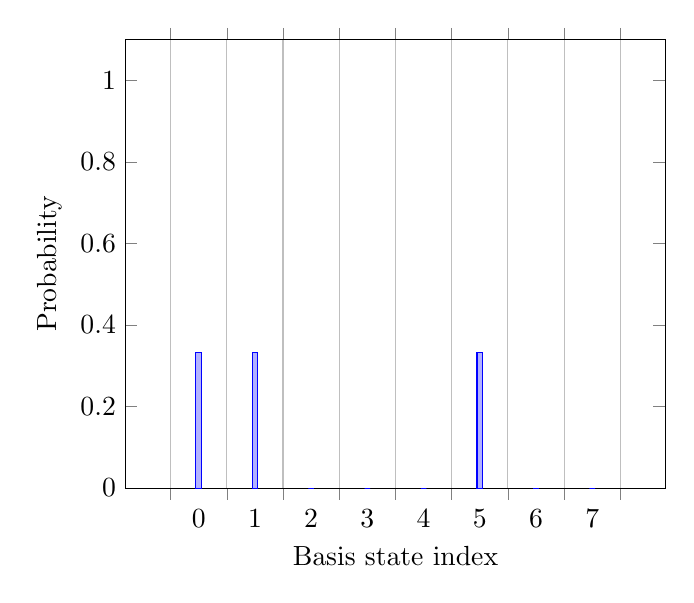
\begin{tikzpicture}
				\begin{axis}[
					ylabel = Probability,
					xlabel = Basis state index,
					ymin = 0,
					ymax = 1.1,
					ybar,
					ybar interval=0.1
				]
				\addplot 
					coordinates {(0,0.333333333333) (1,0.333333333333) (2,0) (3,0) (4,0) (5,0.333333333333) (6,0 ) (7,0) (8,1)};
				\end{axis}
			\end{tikzpicture}
			\caption{Probability distribution for convolution of $\text{T}_a = 11000100$ and $\overline{\text{P}}_a = 10000000$.}
			\label{fig:convolution-a-appendix}
		\end{figure}
	
Again, note that $0.333333333333 = \frac{1}{3}$ and $3.85185988877e^{-34} \approx 0$. Then, the only possible resulting values of a measurement operation on the current state of register $\alpha$ will be the indices 0, 1 and 5. These values correspond to the substrings $\text{T}_a[0, 0] = 1$, $\text{T}_a[0,1] = 11$ and $\text{T}_a[3,5] = 001$.
\end{example}

\begin{example}
\label{exa:aqc-b}
We compute for the convolution of the binary indicator sequences $\text{T}_b$ and $\overline{\text{P}}_b$ given the superposition states $\vert \alpha_b \rangle_0$ and $\vert \beta_b \rangle_0$.
\begin{enumerate}
	\item $\vert \alpha_{b} \rangle_1 = QFT\vert \alpha_{b} \rangle_0 $
		\begin{align*}
			&= QFT \left( \sqrt{\frac{1}{3}}\vert 010 \rangle + \sqrt{\frac{1}{3}}\vert 011 \rangle + \sqrt{\frac{1}{3}}\vert 100 \rangle \right) \\
			&= \left(0.612372435696 \right) \vert 000 \rangle + \left( -0.348461712529 - 0.348461712529\ i \right) \vert 001 \rangle\\
			& \quad + \left( 0.204124145232\ i \right) \vert 010 \rangle + \left( -0.0597865779345 + 0.0597865779345\ i \right) \vert 011 \rangle\\
			& \quad + \left( 0.204124145232 \right) \vert 100 \rangle + \left( -0.0597865779345 - 0.0597865779345\ i \right) \vert 101 \rangle\\
			& \quad + \left( -0.204124145232\ i \right) \vert 110 \rangle + \left( -0.348461712529 + 0.348461712529\ i \right) \vert 111 \rangle
		\end{align*}
	\item $\vert \beta_{b} \rangle_1 = QFT\vert \beta_{b} \rangle_0$
		\begin{align*}
			&= QFT \left( \sqrt{\frac{1}{2}}\vert 001 \rangle + \sqrt{\frac{1}{2}}\vert 010 \rangle \right)\\
			&= \left( 0.5 \right) \vert 000 \rangle + \left( 0.176776695297 - 0.426776695297\ i \right) \vert 001 \rangle\\
			& \quad + \left( -0.25 - 0.25\ i \right) \vert 010 \rangle + \left( -0.176776695297 + 0.0732233047034\ i \right) \vert 011 \rangle\\
			& \quad + \left( 0 \right) \vert 100 \rangle + \left( -0.176776695297 - 0.0732233047034\ i \right) \vert 101 \rangle\\
			& \quad + \left( -0.25 + 0.25\ i \right) \vert 110 \rangle + \left( 0.176776695297 + 0.426776695297\ i \right) \vert 111 \rangle
		\end{align*}
	\item $\vert \alpha_{b} \rangle_2 = V_\beta \vert \alpha_{b} \rangle_1$
		\begin{align*}
			&= V_\beta \Big( \left( 0.5 \right) \vert 000 \rangle + \left( 0.176776695297 - 0.426776695297\ i \right) \vert 001 \rangle\\
			& \quad + \left( -0.25 - 0.25\ i \right) \vert 010 \rangle + \left( -0.176776695297 + 0.0732233047034\ i \right) \vert 011 \rangle\\
			& \quad + \left( 0 \right) \vert 100 \rangle + \left( -0.176776695297 - 0.0732233047034\ i \right) \vert 101 \rangle\\
			& \quad + \left( -0.25 + 0.25\ i \right) \vert 110 \rangle + \left( 0.176776695297 + 0.426776695297\ i \right) \vert 111 \rangle \Big)\\
			&= \left( 0.612372435696 \right) \vert 000 \rangle \\
			& \quad + \left( -0.455287168268 + 0.188586119871\ i \right) \vert 001 \rangle \\
			& \quad + \left( 0.144337567297 - 0.144337567297\ i \right) \vert 010 \rangle \\
			& \quad + \left( 0.0323562628193 - 0.0781149285259\ i  \right) \vert 011 \rangle \\
			& \quad + \left( 0.204124145232\ i \right) \vert 100 \rangle \\
			& \quad + \left( 0.0323562628193 + 0.0781149285259\ i  \right) \vert 101 \rangle\\
			& \quad + \left( 0.144337567297 + 0.144337567297\ i \right) \vert 110 \rangle \\
			& \quad + \left( -0.455287168268 - 0.188586119871\ i \right) \vert 111 \rangle 
		\end{align*}
	\item $\vert \alpha_{b} \rangle_3 = QFT^{-1}\vert \alpha_{b} \rangle_2$
		\begin{align*}
			&= QFT^{-1}\Big( \left( 0.612372435696 \right) \vert 000 \rangle + \left( -0.455287168268 + 0.188586119871\ i \right) \vert 001 \rangle \\
			& \quad + \left( 0.144337567297 - 0.144337567297\ i \right) \vert 010 \rangle \\
			& \quad + \left( 0.0323562628193 - 0.0781149285259\ i  \right) \vert 011 \rangle + \left( 0.204124145232\ i \right) \vert 100 \rangle \\
			& \quad + \left( 0.0323562628193 + 0.0781149285259\ i  \right) \vert 101 \rangle\\
			& \quad + \left( 0.144337567297 + 0.144337567297\ i \right) \vert 110 \rangle \\
			& \quad + \left( -0.455287168268 - 0.188586119871\ i \right) \vert 111 \rangle \Big)\\
			&= (0.0195111123457 + 0.0721687836487\ i ) \vert 000 \rangle \\
			& \quad + (0.0195111123457 - 0.0721687836487\ i) \vert 001 \rangle \\
			& \quad + (-0.074141841541 + 0.0721687836487\ i) \vert 010 \rangle \\
			& \quad + (0.303030398201 - 0.0721687836487\ i) \vert 011 \rangle \\
			& \quad + (0.617625734778 + 0.0721687836487\ i) \vert 100 \rangle \\
			& \quad + (0.617625734778 - 0.0721687836487\ i) \vert 101 \rangle \\
			& \quad + (0.303030398201 + 0.0721687836487\ i) \vert 110 \rangle \\
			& \quad + (-0.074141841541 - 0.0721687836487\ i) \vert 111 \rangle
		\end{align*}
\end{enumerate}
The final state of register $\alpha$ which represents the convolution of the binary indicator sequences $\text{T}_b$ and $\overline{\text{P}}_b$ will be the quantum superposition state $\vert \alpha_{b} \rangle_3$. Each substring $\text{T}_b [j-M-1,j]$ compared to $P_b = 110$ such that $\text{T}_b [j]$ is aligned with $\text{P}_b[M-1]$, and their corresponding basis state's amplitude and probability are shown in Table~\ref{tab:convolution-b-appendix}. A probability distribution corresponding to the convolution of $\text{T}_b$ and $\overline{\text{P}}_b$ is shown in Figure~\ref{fig:convolution-b-appendix}.

	\begin{table}[h!]
	\begin{center}
	\begin{tabular}{|| c | c | c | c ||}
		\hline 
		\textit{j} & $\text{T}_b [j-M-1,j]$ & $\langle i \vert \alpha_{b_3} \rangle$ &  $\vert \langle i \vert \alpha_{b_3} \rangle \vert^2$\\
		\hline\hline
			0 & 0	  & 0.0195111123457 + 0.0721687836487\ i & 0.0055890168383\\
		\hline
			1 & 00   & 0.0195111123457 - 0.0721687836487\ i & 0.0055890168383\\
		\hline
			2 & 001 & -0.074141841541 + 0.0721687836487\ i & 0.0107053460004\\
		\hline
			3 & 011 & 0.303030398201 - 0.0721687836487\ i   & 0.0970357555674\\
		\hline
			4 & 111 & 0.617625734778 + 0.0721687836487\ i  & 0.386669881594\\
		\hline
			5 & 110 & 0.617625734778 - 0.0721687836487\ i   & 0.386669881594\\
		\hline
			6 & 00   & 0.303030398201 + 0.0721687836487\ i  & 0.0970357555674\\
		\hline
			7 & 0    & -0.074141841541 - 0.0721687836487\ i  & 0.0107053460004\\
		\hline
	\end{tabular}
	\end{center}
	\caption{Comparison result between $\text{T}_b = 001110$ and $P_b = 110$.}
	\label{tab:convolution-b-appendix}
	\end{table}

		\begin{figure}
			\centering
			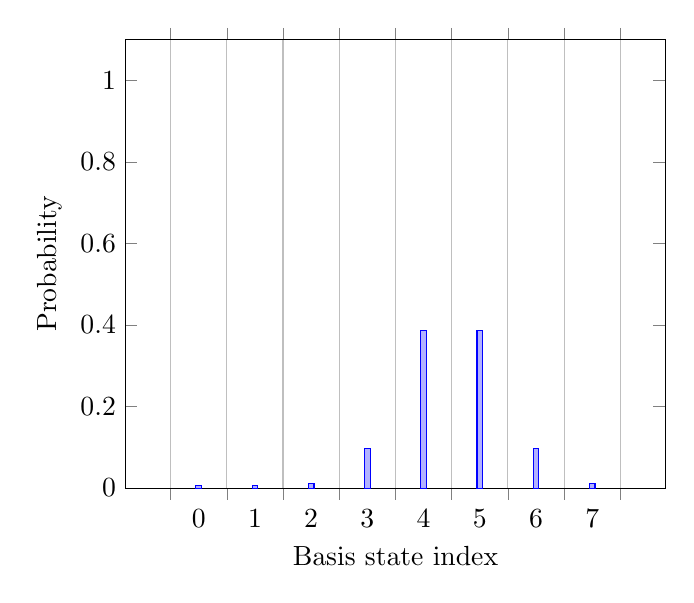
\begin{tikzpicture}
				\begin{axis}[
					ylabel = Probability,
					xlabel = Basis state index,
					ymin = 0,
					ymax = 1.1,
					ybar,
					ybar interval=0.1
				]
				\addplot 
					coordinates {(0,0.0055890168383) (1,0.0055890168383) (2,0.0107053460004) (3,0.0970357555674) (4,0.386669881594) (5,0.386669881594) (6,0.0970357555674 ) (7,0.0107053460004) (8,0)};
				\end{axis}
			\end{tikzpicture}
			\caption{Probability distribution for convolution of $\text{T}_b = 00111000$ and $\overline{\text{P}}_b = 01100000$.}
			\label{fig:convolution-b-appendix}
		\end{figure}

As shown in Table~\ref{tab:convolution-b-appendix} the substrings $\text{T}_b [j-M-1, j]$ with highest probability of occurring from a measurement operation of state of register $\alpha$ are first those for which $j=4$ and $j=5$, followed by those for which $j=3$ and $j=6$, then that for which $j=7$ and $j=2$ and lastly, that for which $j=1$ and $j=0$.
\end{example}

            % \include{appendix/circuit}
            % \chapter{Simulation Source Code in Python}
        
        \end{document}